% Szkielet dla pracy inżynierskiej pisanej w języku angielskim.

\documentclass[english,bachelor,a4paper,oneside]{ppfcmthesis}

\usepackage[utf8]{inputenc}
\usepackage[OT4]{fontenc}
\usepackage{amsmath}
\usepackage{color}
\usepackage{listings}
\usepackage{epstopdf}

\DeclareMathOperator*{\argmax}{arg\,max}
%\newcommand{\argmax}{\operatornamewithlimits{argmax}}

% Authors here.
\author{%
   Michał Nowicki \album{95883} \and 
   Olgierd Pilarczyk \album{100449} \and 
   Jakub Wąsikowski \album{101560} \and 
   Katarzyna Zjawin \album{98826}}
\authortitle{}                                        % Do not change.
\title{Gesture recognition library for Leap Motion Controller}        % Note how we protect the final title phrase from breaking
\ppsupervisor{dr~inż.~Wojciech Jaśkowski} % Your supervisor comes here.
\ppyear{2014}                                         % Year of final submission (not graduation!)

\begin{document}

% Front matter starts here
\frontmatter\pagestyle{empty}%
\maketitle\cleardoublepage%

% Blank info page for "karta dyplomowa"
\thispagestyle{empty}\vspace*{\fill}%
\begin{center}Tutaj przychodzi karta pracy dyplomowej;\\oryginał wstawiamy do wersji dla archiwum PP, w pozostałych kopiach wstawiamy ksero.\end{center}%
\vfill\cleardoublepage%

% Table of contents.
\pagenumbering{Roman}\pagestyle{ppfcmthesis}%
\tableofcontents* \cleardoublepage%

% Main content of your thesis starts here.
\mainmatter%

\chapter{Streszczenie}
Niniejsza praca jest poświęcona nowym możliwościom zastosowania gestów do interakcji człowieka z komputerem, które pojawiły się wraz z wprowadzeniem na rynek urządzenia Leap Motion.
Leap Motion to innowacyjne urządzenie, które udostępnia dane dotyczące pozycji rąk oraz palców w przestrzeni trójwymiarowej z dokładnością do $0,01$mm.
Głównym rezultatem niniejszej pracy jest przeznaczona dla programistów, dedykowana dla kontrolera Leap Motion, biblioteka LeapGesture udostępniona na licencji open-source, która zawiera algorytmy do nauki oraz rozpoznawania gestów.
Autorzy pracy zbadali możliwości sensora w zastosowaniu rozpoznawania układów dłoni (gestów statycznych), wykonywanych ruchów ręki (gestów dynamicznych) oraz rozróżniania palców.
Statyczne gesty są rozpoznawane za pomocą mechanizmu maszyn wektorów wspierających (SVM) z wykorzystaniem filtracji medianowej danych wejściowych oraz przy wykorzystaniu zależności pomiędzy kolejnymi rozpoznanymi gestami w danym oknie czasowym.
Praca zawiera także badania różnych używanych wektorów cech, których wybór ma znaczny wpływ na uzyskiwane rezultaty.
Zaproponowane podejście do wybranych cech umożliwiło rozpoznawanie zbioru gestów należących do pięciu klas z dokładnością $99\%$ oraz zbioru gestów należących do dziesięciu klas z dokładnością $85\%$.
Gesty dynamiczne (ruch ręki oraz palców) są rozpoznawane za pomocą ukrytych modeli Markowa (HMM).
Przyjęte podejście umożliwiło osiągnięcie $80\%$ skuteczności rozpoznawania gestów dynamicznych należących do sześciu klas.
Moduł rozróżniania palców ręki dla badanych zbiorów osiągnął dokładność rozpoznawania wynoszącą $93\%$. 
W bibliotece zostały zaimplementowane wyżej wymienione podejścia w języku C++, dzięki czemu biblioteka LeapGesture może być użyta w aplikacji każdego typu.

\chapter{Abstract}
This thesis studies the new possibilities to gesture interfaces that emerged with a Leap Motion sensor.
The Leap Motion is an innovative, 3D motion capturing device designed especially for hands and fingers tracking with precision up to $0.01$mm.
The main outcome of the thesis is the open-source LeapGesture library dedicated to the developers for Leap Motion Controller that contains algorithms allowing to learn and recognize gestures.
The authors examined the data provided by the sensor in context of recognition of hand poses (static gestures), hand movements (dynamic gestures) and in task of a finger recognition.
The static gestures are recognized using the Support Vector Machine (SVM) with median filtering an input data and using the correspondences between consecutive recognitions.
The proposed approach allowed to recognize a set of five gestures with $99\%$ accuracy and a set of ten gestures with $85\%$.
The dynamic gestures (movements of a hand and fingers) are recognized with the Hidden Markov Models (HMM). 
Recognition with HMMs allowed to achieve accuracy of $80\%$ for a set containing six dynamic gestures.
Finger recognition algorithms proposed in this thesis works with $93\%$ accuracy on a recorded dataset.
The LeapGesture library contains presented approaches using a C++ interface, that can be easily used in every application.
\chapter{Introduction}

\section{Motivation}

Nowadays, human-computer interaction is mainly based on the pointing or typewriter-style devices. 
This kind of interaction can limit the natural ways of manipulation using the hands, which may result in a complication of simple tasks.
One of the overcomplicated control examples is rotating a three-dimensional object.
Using a computer mouse, a user needs to grab the object and rotate it using the mouse, which can only operate in a two-dimensional space. 
The rotation operation represented by the mouse's movement is unintuitive for humans and users need a few attempts to understand how it works. 
In the real world, however, the rotation task is natural thus it is simple how to move hands to rotate the object in a desired way.

Therefore, there exists a need for more natural human-computer interfaces.
One of the proposed approaches involves hand gestures that are interpreted by a computer.
Utilizing hands in a human-computer interface is supported by the fact, that they are even used for non-verbal communication, such as sign or body language.
The another advantage of hands is that manipulative tasks performed using hands in real the world could be interpreted as a series of gestures and used as computer input.

The newest sensors provide data that can be successfully used to recognize gestures and therefore control a computer.
Currently, there are several devices that yield data useful for the gesture recognition. 
An example of such a controller is Microsoft Kinect.
It provides a three-dimensional image of the observed scene, but was designed for applications that interpret the movement of the whole body of the user. 
That is why it lacks the needed accuracy for hand gesture recognition.
 
Another device that is designed to track the movements of a hand and fingers is Leap Motion Controller developed by Leap Motion, Inc. released in July 2013. 
The Leap Motion is a small device, which can be placed in front of a computer. It features extreme finger detection accuracy up to 0.01 mm. 
The controller provides information about a position of each finger and a hand detected in the observed space.
The SDK attached to the device allows to recognize three pre-defined gestures: a circle motion with one finger, a swipe action and tapping on the virtual keys. 
The Leap Motion Controller provides information about every detected hand. This device transmits data with frequency up to 100~Hz. 
Leap Motion Controller is a sensor that can potentially revolutionize the human-computer interactions. 

Currently, there exists no library for gesture recognition that supports the data provided by the Leap Motion Controller.
This is an important limitation when creating Leap Motion-based applications.
Right now, when developers want to create applications utilizing the gesture recognition, they need to operate on low-level, unprocessed data and need to implement the gesture recognition on their own.
This additional work overhead could be minimized using high-level library.

\section{Objectives}

Therefore, the goal of this thesis is to develop the library for gesture recognition dedicated to Leap Motion device, which will help developers to implement applications using gestures as a human-computer interface.

The goal will be achieved by meeting the following objetives:
\begin{itemize}
\item to design the library architecture, 
\item to compare existing methods in the context of hand gesture recognition,
\item to select and implement algorithms for gesture recognition,
\item to implement additional modules enabling the recording and reviewing of gestures saved in a format supported by the library,
\item to create a sample gestures database,
\item to perform gesture recognition tests using Leap Motion Controller.
\end{itemize}
The additional requirement of the library is that the processing should be realized in real time.


The recognition modules are based on Support Vector Machines (SVM) and Hidden Markov Models (HMM). 
SVM is a supervised learning algorithm, which uses set of hyperplanes for non-linearly division of input vectors to different classes. 
HMM is an example of an unsupervised learning algorithm, where model tries to find a hidden structure of data using provided training samples. 
Algorithms used in this thesis belong to a group of machine learning algorithms.

The thesis was developed from October 2013 till January 2014.


\section{Thesis organization}
The thesis is structured in the following manner. 
Chapter~\ref{introGRChapter} contains an overview of the literature concerning the gesture recognition problem. 
This part includes descriptions of gestures taxonomies and state of the art methods used for gesture recognition.
The presentation of Leap Motion Controller is in Chapter~\ref{LMCChapter}.
Chapter~\ref{GestureRecChapter} is devoted to gestures recognizing in the context of Leap Motion Controller.
It contains also descriptions of gestures classification, data representations and additional processing steps for hand gestures recognition using the Leap Motion device. 
The following Chapter~\ref{staticChapter} describes proposed methods, evaluation methodology and experiments for static gesture recognition. 
Chapter~\ref{dynamicChapter} presents a description of dynamic gesture recognition. 
Chapter~\ref{libraryChapter} contains a description of the created library --- its architecture, processes, modules, dependencies on other open-source libraries, and an example of its usage. 
Chapter~\ref{conclusionsChapter} concludes the thesis and provides possible future works. 

\section{Contributions}
Michał Nowicki:
\begin {itemize} 
\item described dynamic gestures (Chapter~\ref{dynamicChapter}),
\item described static gestures (Chapter~\ref{staticChapter} expect Section~\ref{fingerSection}), 
\item implemented code of processing algorithms for static and dynamic gestures recognition without an integration into the library,
\item performed experiments evaluating the static and dynamic gesture recognition. 
\end {itemize}

Olgierd Pilarczyk:
\begin{itemize}
\item wrote the description of Leap Motion controller (Chapter~\ref{LMCChapter}),
\item described data models (Section~\ref{datarepSection}), data preprocessing (Section~\ref{PreprocessingSection}),
\item described library architecture (Section~\ref{architectureSection} expect Subsection~\ref{modelSubsection}, Section~\ref{librariesSection}, Section~\ref{sampleSection}),
\item implemented preprocessing and integration dynamic gesture module to library. 
\end {itemize}

Jakub Wąsikowski:
\begin {itemize}
\item wrote the introduction to gesture recognition (Chapter~\ref{introGRChapter}),
\item described classification of gestures (Section~\ref{classificationSection}) and confusion matrix of static gestures,
\item participated in research and definition of gesture classification,
\item implemented finger recognition, recorder and vizualizer, model and format of gestures recordings, determining the number of clusters for dynamic gestures, class for cross validation, integration static gesture and finger recognition modules to library.
\end{itemize}

Katarzyna Zjawin: 
\begin{itemize}
\item wrote the introduction (Chapter~\ref{introGRChapter}),
\item described finger recognition (Section~\ref{fingerSection}),
\item described the data model (Subsection~\ref{modelSubsection}), processes (Section~\ref{processesSection}), recorder and visualizer (Section~\ref{recordvisualSection}),
\item participated in research and definition of gesture classification,
\item implemented and tested finger recognition,
\item implemented recorder and visualizer, model and format of gestures recordings.
\end{itemize}



\chapter{Introduction to gesture recognition}

\section{Taxonomies of gestures proposed in literature}
The vast multiplicity of gestures that human can perform makes the number of classes to which we can divide these gestures substantial. Therefore the classification can be performed in different ways, taking into account different characteristics of gestures. The majority of presented theories include the knowledge that originates from a variety of science such as anthropology, linguistics, cognitive science and other. In this Section, review of the most common gesture classifications in Human Computer Interaction (HCI) context is provided. It is focused mainly on gestures that relate to hand and arm movements.

The basic classification of gestures is the division into static and dynamic gestures. Group of static gesture includes fixed gestures which are not take into account the changes in time. Dynamic gestures is group of time varying gestures.

There is also another general division considered by Kammer et al. \cite{kammer_taxonomy_2010} due to the type of actions activated by the gesture, to online and offline. The first group includes gestures which are processed during performing. It is the group of direct manipulation gestures that provide additional information about dynamics of gesture. They are often used to manipulate objects in space. The second one is the group of action gestures, which are processed at the end of gesture. Most often these are gestures that convey the occurrence of specific meaning.

Karam and schraefel \cite{Karam05ataxonomy} proposed more extensive gesture taxonomy dedicated for Human Computer Interaction. Their classification is based on Quek et al. \cite{Quek:2002:MHD:568513.568514} publication, which provides clarification of gestures taxonomies presented in the past literature. Karam and schraefel defined following gesture classes: deictic, gesticulation, manipulation, semaphores and sign language. In another publication, Aigner et al. \cite{AignerTaxonomy} presented classification, which are more tailored for hand gesture recognition purposes, drawing on concepts from Karam and schraefel work. They distinguished five categories of gestures:

\begin{figure}[htb]
\centering
 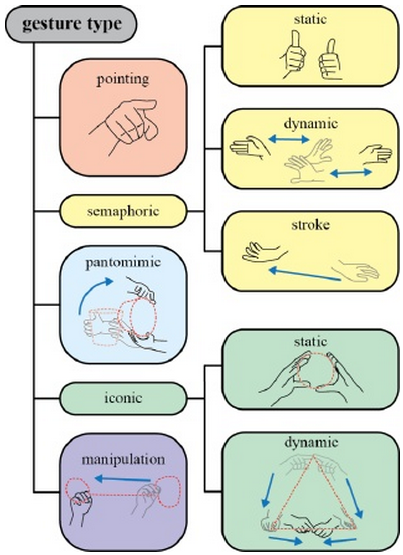
\includegraphics[width=0.5\columnwidth]{figures/gestureTypes.png}
 \caption[]{The classification of gestures proposed by Aigner et al. \cite{AignerTaxonomy}}
 \label{gesturetypes}
\end{figure}

\begin{itemize}

\item pointing -- used to point object or indicate direction. Formally, it involve pointing to establish the identity or spatial location of an object within the context of the application domain \cite{Karam05ataxonomy}. This applies not only to indicate by the index finger, but also by any finger or any number of fingers. It is also independent of finger orientation and curvature, while gesture has a indication meaning. Equivalent to deictic gesture in Karam and Schraefel literature.

\item semaphoric -- group which consists of gesture posture and dynamics of gesture, which are used to convey specific meanings. Formally, semaphoric approaches may be referred to as ``communicative'' in that gestures serve as a universe of symbols to be communicated to the machine \cite{Quek:2002:MHD:568513.568514}. Due to the fact that semaphoric are symbolic gestures, their layout can be unrelated to their meaning. Distinguished three semaphoric gesture types of static, dynamic and strokes. The first one concerns specific hand posture, such as thumbs-up meaning approval symbol.
Dynamic semaphorics convey their meaning through movement, for example waving of hand to greet somebody. The last one group are similar to dynamic semaphorics gesture, but this represents fast, stroke-like movements, such as swipe gesture.

\item iconic -- used to demonstrate shape, size, curvature of object or entities. In contrast to the semaphoric gestures, their layout or motion path is strictly related to their meaning. Iconic gestures can be divided into static and dynamic. The former group is performed by hand postures, such as rectangle formed by the thumb and forefingers of both hands. The latter group is often used to map edge line of objects by means of motion paths. For instance showing a simplified sine function characteristics with finger movements.

\item pantomimic -- used to imitate performation of specific task or activity without any tools or objects. Pantomimic gesture are characterized by a high variability of posture and movements. An example of this gesture type can be weapon reload or movement of a knife slicing bread.

\item manipulation -- used to control the position, rotation and scale of the object or entity in space. Manipulation gestures constitute a direct interaction between the manipulated object and a hand or a tool that performs gesture. It follows, that the movement of the manipulated object must be strictly dependent on the motion gesture.
\end{itemize}

\section{State of the art methods}
In this Section, review of the state-of-the-art in human gesture recognition is presented. The problem of gesture recognition can be divided in two main problems: the gesture representation problem and the decision/inference problem. Therefore, this review includes discussion about enabling technology, gesture representations and analysis of recognition methods. Additionally, general problems related to the recognition of gestures and their common solutions are introduced.

\subsection{Sensors}
In this Subsection, the sensors for gesture recognition are overviewed. The main existing gesture recognition approaches related to type of the devices are as follow:
\begin{itemize}
\item non-vision-based devices -- tracking devices, instrumented gloves, armbands and others,
\item vision-based devices -- using one or many cameras.
\end{itemize}

\subsubsection{Non-vision-based Sensors}

This type of devices use various technologies to detect motions, such as accelerometers, multi-touch screens, EMG sensors and other, which include different types of detectors. There are few categories of non-vision-based devices \cite{kaaniche2009human}:

\begin{itemize}

\item wearable -- this kind of device is in the form of garment, which includes sensors needed to recognize arrangement and motions of examined part of the body. It often occur in the form of gloves (CyberGlove®), armband (Myo) or the whole outfit (IGS-190). For instance, CyberGlove® device was used in the system developed by Kevin et al. \cite{KevinCyberGloves}, which recognizes multi-dimensional gestures using condensation-based trajectory matching algorithm. These devices are often related to biomechanical and inertial technologies, 

\item biomechanical -- type of device, which use biomechanical techniques such as electromyography, to measure parameters of gesture. An example of using this type of device is the project developed by Kim et al. \cite{Kim:2008:EHG:1378773.1378778} for Realtime Biosignal Interfacing based on EMG sensors. Example of these devices is Myo armband, which detects gestures and movements using EMG sensors,

\item inertial -- these devices measure the variation of the earth magnetic field in order to detect the motion. This kind of devices use accelerometers \cite{LiuAccelerometer} and gyroscopes \cite{TUD-CS-2009-0292} to measurements,

\item haptics -- various kinds of touch screens. For instance, Webel et al. \cite{conf/vrst/WebelKZ08} developed module for dynamic gestures recognition in multi-touch devices,

\item electromagnetic -- these devices measure the variation of an artificial electromagnetic field generated by wireless networks, electronic devices or produced by themselves. An example of such devices is WiSee, which leverages ongoing wireless transmissions in the environment (e.g., WiFi) to enable whole-home sensing and recognition of human gestures \cite{Pu:2013:WGR:2500423.2500436}.

\end{itemize}

\subsubsection{Vision-based Sensors}

Vision-based sensors include one or several cameras and provide perfomed data from the captured video sequences. Processing of frame is based on filtering, analyzing and data interpreting. The following types of vision-based technology can be distinguished \cite{kaaniche2009human}\cite{Wu:1999:VGR:647591.728702}:

\begin{itemize}

\item typical video cameras -- gesture recognition techniques based on data derived from monocular camera using detection methods such as color or shape based techniques, learning detectors from pixel values or 3D model-based detection,

\item stereocameras -- techniques based on captured images from two cameras, which provide an approximation of the recorded data to a 3D model representation,

\item active techniques -- require the projection of some form of structured light. Examples of this kind devices are Kinect or Leap Motion,

\item invasive techniques -- systems which require using of body markers such as color gloves \cite{Wang:2009:RHC:1531326.1531369}, LED lights (Play Station Move controller).

\end{itemize}

\begin{figure}[htb]
\centering
 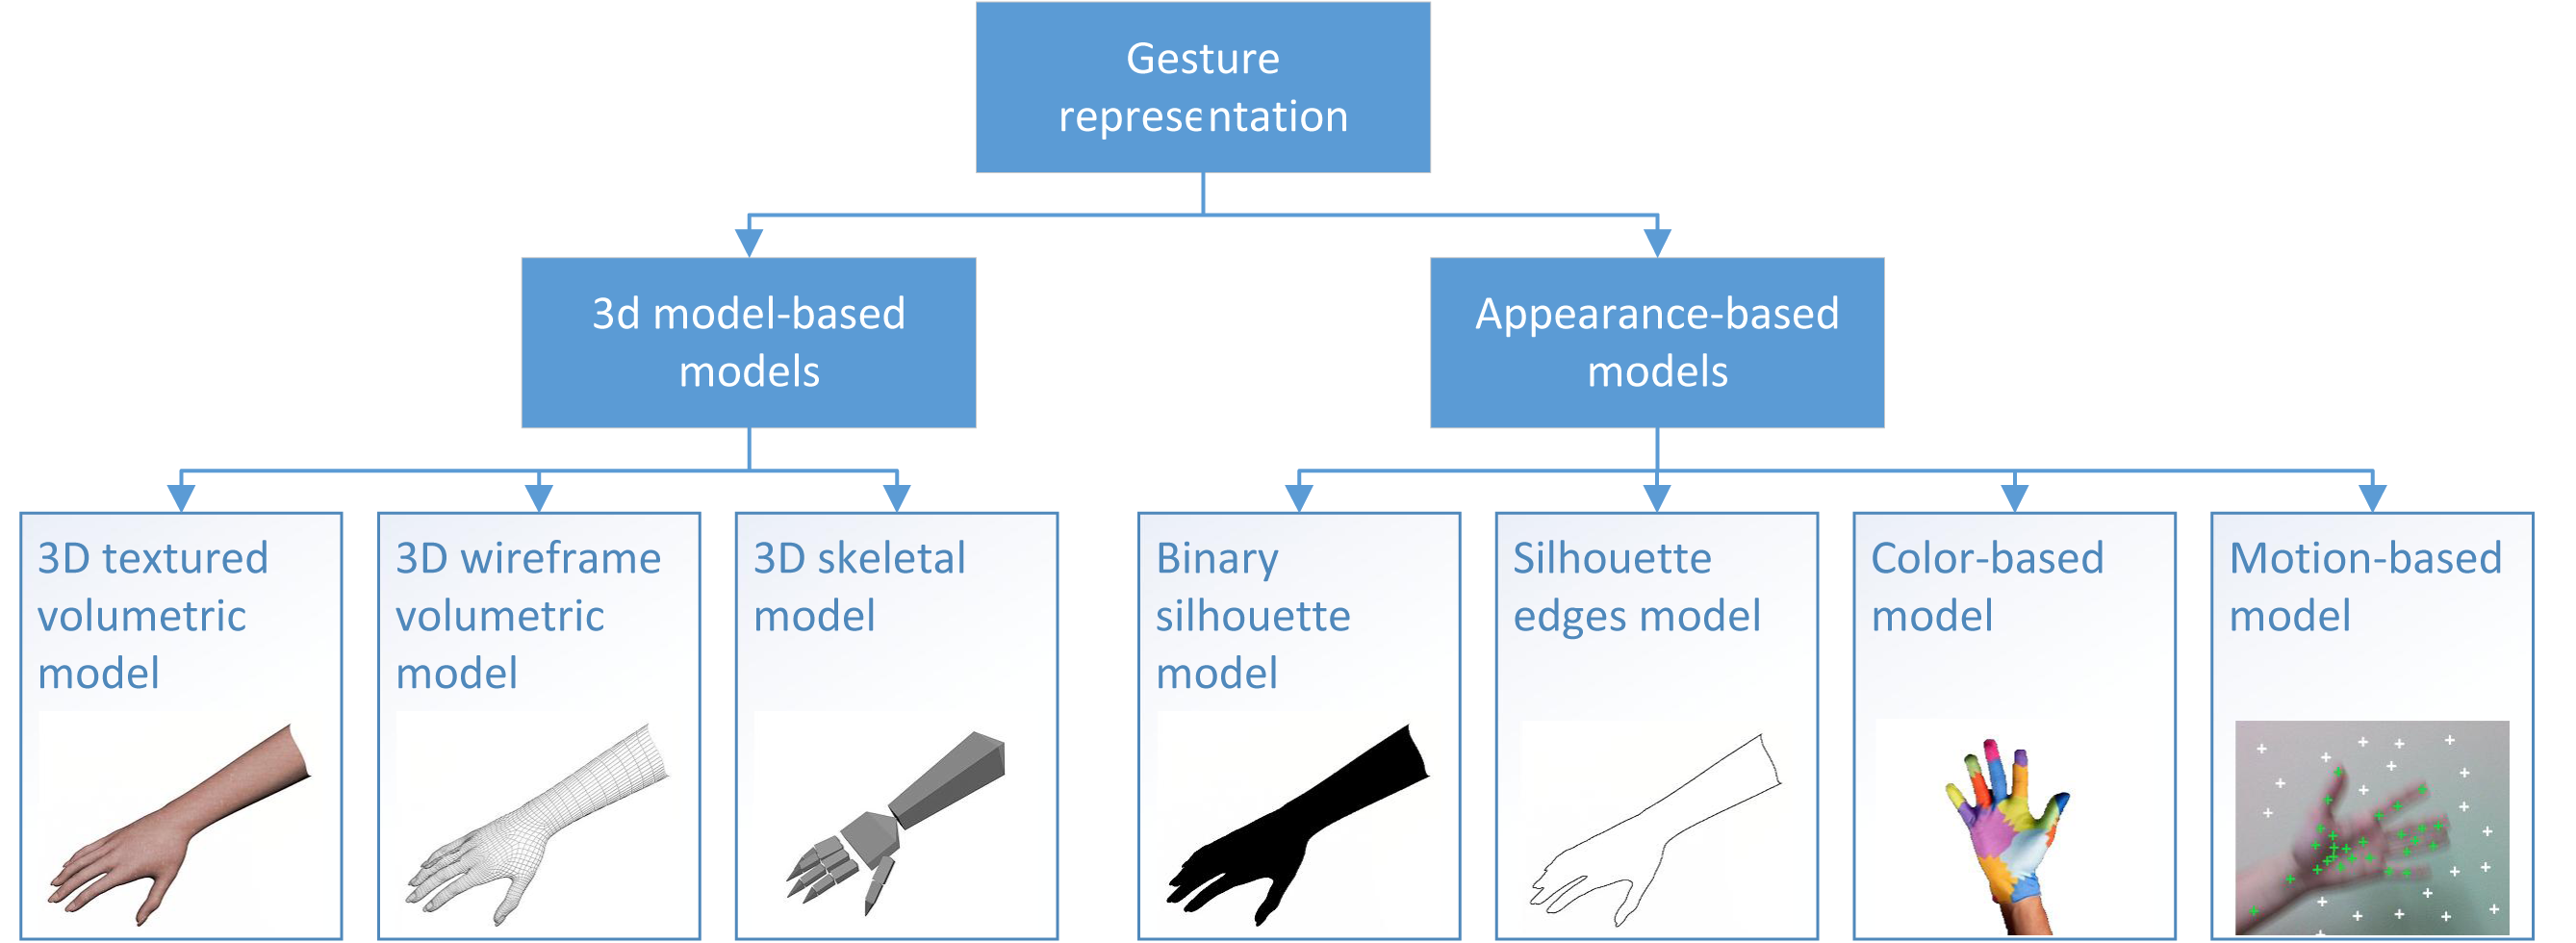
\includegraphics[width=1\columnwidth]{figures/gestureRepresentations.png}
 \caption[]{Diagram of gesture representation}
 \label{gesturerepresentations}
\end{figure}

\subsection{Gesture representation}
In this Subsection, overview the spatial modeling of gestures is provided. In particular, greater importance is placed on one type of spatial gesture representations, called the 3D model-based. Depending on the type of the input data, the approach for recognize gesture could be done in different ways.
There are following two main types of gesture representation defined in literature \cite{Huang95handgesture}\cite{Pavlovic97visualinterpretation}:
\begin{itemize}
\item 3d model-based,
\item appearance-based.
\end{itemize}

\subsubsection{3D model-based}

Defines the 3D spatial decription of the human body parts. They can be classified in two large groups:
\begin{itemize}
\item volumetric models,
\item skeletal models.
\end{itemize}
Volumetric models reproduce with high accuracy the shape of the hand or arm. Real object is often interpreted as mesh of vertices or non-uniform rational B-spline (NURBS) ordered in space. This model is commonly used for computer vision purposes or for computer animation. The drawback of this approach is that, it is computationally demanding and difficult to analyze in real time. Simplified models of the hand or arm with the reduced set of parameters (such as skeletal models) are often used \cite{Pavlovic97visualinterpretation}.

As indicated earlier, instead of dealing with all the parameters of volumetric type, model can be reduced to set of equivalent joint angle parameters together with segment lengths. These are known as skeletal models. There are several advantages of using this representation type:
\begin{itemize}
\item Simplified model with the most important parameters allows the detection program to focus on the significant parts of the body.
\item Due to the smaller amount of data, the processing algorithms are faster.
\end{itemize}

\subsubsection{Appearance-based}

The second group of models do not use direct description of the spatial object points, because this model is based on shape of hands or arms in the visual images. The gestures are modeled by relating the appearance of any gesture to the appearance of the set of predefined, template gestures \cite{Pavlovic97visualinterpretation}. In this group distinguished a large variety of models. The most used 2D models are:
\begin{itemize}
\item color based model -- in general, using body markers to track the motion of the body part,
\item binary silhouette based model -- models based on the geometric properties of the object silhouette,
\item deformable gabarit based model -- they are generally based on deformable active contours,
\item motion-based model -- based on the motion of individual pixels or image part description.
\end{itemize}

\subsection{Gesture recognition methods}\label{DynamicStaticText}
As it was written earlier, one of the main issues of gesture recognition is the decision problem. Currently several solutions have been proposed, which can be used regardless of device type or data representation for different classes of gestures. Classification of gestures, which should be taken into account while choosing gesture recognition method, are static and dynamic division. For each of them may be used different tools due to the different properties of these gestures. In the case of static gesture recognition, an important feature is arrangement of object, which performs a gesture, in other words, how the individual parts of the object are arranged in relation to each other. For dynamic gestures --- as described in the previous Subsection --- a very important feature is the variation in time (dynamics of the gesture or dynamics of individual parts of the object performing the gesture).

To recognize static gestures, general classifier, neural network or template-matcher can be used. Methods which are capable to recognize dynamic gestures have to take into account the aspect of time. An example of this kind of method is Hidden Markov Model.

\subsubsection{Static gesture recognition}

Different techniques to perform accurate static gesture recognition have been decribed in the literature. The most common methods are neural networks, support vector machines and simple pattern techniques \cite{journals/jbcs/SavarisW10}.

\emph{A neural network (NN)} is an information-processing system that has been developed as generalizations of mathematical models of human cognition or neural biology. A neural network is characterized by its pattern of connections between the neurons, method of determining the weights on the connections, and its activation function \cite{Fausett:1994:FNN:197023}. They can be used both for static and dynamic gestures.

Hasan et al. \cite{HasanStaticHand} presented hand gesture recognition based on shape analysis. Tests were conducted for six static gestures using multi-layer perception of neural network and back-propagation learning algorithm. NN architecture consisted of one hidden layer ($100$ nodes), $1060$ inputs and $6$ output for each gesture. They achieved a recognition rate of $86.38\%$ for a training set of $30$ images and a testing set of $84$ images.

Xu et al. \cite{conf/icat/XuYZ06} developed virtual training system of Self-Propelled Gun based on static gesture recognition and hand translations and rotations. The input data for algorithms was captured using a $18$-sensor DataGlove. To recognize gestures was used feed-forward neural network with $40$ nodes in single hidden layer, $18$ input and $15$ output nodes. The back-propagation using a variable learning rate is selected as training method. The tests were conducted on a set of $300$ hand gestures from five different people --- $200$ gestures for training set and $100$ for testing set. With the use of these methods the authors reached gesture recognition performance of $98\%$.

In publication of Stergiopoulou and Papamarkos publication \cite {Stergiopoulou:2009:HGR:1651923.1651954} can be found static gesture recognition through other type of neural network --- Self-Growing and Self-Organized Neural Gas (SGONG). To quote the authors, SGONG is innovative neural network that grows according to the morphology of hands in a very robust way. The algorithms were tested for $31$ hand gestures that derive from the combination of shown and hidden fingers. Data were collected from a camera, and the recordings of hand were created in a vertical position on uniform background. With these assumptions, gesture recognition rate of $90.45\%$ have been reached but required average computation time was about $1.5$ s, using a $3$ GHz CPU.

\emph{Support-Vector Machine (SVM)} is a classification method invented by Vapnik \cite{Cortes:SVM}. SVM is a supervised learning algorithm used for classification and regression analysis, based on the mapping of characteristics extracted from instances namely the feature vectors to points in space. SVM constructs in multi-dimensional space, set of hyperplanes, which non-linearly divide points in this space (input vectors) to different classes. Support Vector Machines can be called a maximum margin classifier, because the resulting hyperplanes maximize the distance between the ’nearest’ vectors of different classes. These ``nearest'' vectors are called support vectors.

Chen and Tseng \cite{ChenDeveloping} presented system based on training SVM which allows effective recognition gesture in popular game, rock-paper-scissors. One of the challenges of their work was to teach the classifier to recognize multiple-angle hand gesture. The collection of training and testing data were images from video camera, which are preprocessed using convertion to grayscale and histogram equalization. Data were collected from $5$ different people for the right hand only. For the learning set consisted of $420$ images and testing set of $120$ images, the recognition rate of $95\%$ was achieved.

Rahman and Afrin \cite{RahmanHand} presented hand gesture recognition system which recognizes static hand gesture for alphabet of $10$ letters using Biorthogonal Wavelet Transform and SVM. Input data in the form of images --- in addition to filtering --- are transformed by the Canny edge detection method and then processed sequentially through Radon and Biorthogonal Wavelet Transformations. Finally, the data in this form are transmitted to the SVM classifier. To achieve robustness of the method to varying conditions, authors used a large dataset --- $800$ positive samples and $1500$ negative image samples. Average recognition rate was $87.4\%$.

Liu et al. \cite{LiuStatic} proposed recognition method based on SVM and Hu moments which applied to Chinese Driver Physical Examination System. For collection of $2416$ positive samples and $3050$ negative samples from $20$ people recognition rate of $96.5\%$ have been reached.

Ren and Zhang \cite{RenMEBSVM} proposed other recognition method named by them as MEB-SVM. This method combines the SVM with minimum enclosing ball (MEB) and --- according to the authors --- allows to reduce computation with effective separation of all kinds of vectors in hyperspace. The input data used to test this method are images which are initially binarized and then countour line is retrieved. Finally, contour line is converted by means of Fourier transform, so that data are independent of translation, rotating and zooming. Their method achieved a recognition rate of $92.9\%$.


Dominio et al. \cite{Dominio:2013:HGR:2510650.2510651} presented novel hand gesture recognition based on depth data using Kinect device. The proposed processing consists following, main steps: extraction hand region from the depth map and subdivided it into palm and finger samples, extraction set of features based on finger tips and center of the hand, classification by SVM. Based on $1,000$ different depth maps with $10$ gestures performed by $10$ different people, they achieved mean recognition rate of $99.5\%$.

Other popular methods are \emph{simple pattern recognition techniques}. This group includes methods based on a simple comparison the characteristics of new problem instance with instances seen in training, instead of performing explicit generalization. In the case of gesture recognition, output information of algorithm is evaluated on the basis of similarity of the gesture to other pre-defined or learned gestures, for which belonging to groups is known. Basis on this, it is concluded that the newly read gesture belongs to the group. These techniques are generally based on a efficient lazy learning methods such as instance-based learning methods.  In the context of gesture recognition, the most widely used algorithm is the k-nearest neighbour.

Ziaie et al. \cite{ziaie-etal-csicc2008-revised} combine naïve Bayes classifier with k-nearest neighbors algorithm for static gesture recognition purposes. Based on the dataset from the camera consisting of $580$ samples for the $3$ gestures, authors have achieved $93\%$ of recognition rate.

Chang et al. \cite{journals/jise/ChangCTH06} proposed new approach for static gesture recognition based on Zernike moments (ZMS) and pseudo-Zernike moments (PZMs), which provide greater independence from the translation of gestures. For gesture classification, k-nearest neighbor has been used, which directly processes the data from the ZMS and PZMs. In addition, authors used a minimum bounding circle, which supports the decomposition of hand silhouette into the finger parts and palm part. For dataset of $600$ samples with $6$ gestures performed by $10$ people, gesture recognition rate of $97.3\%$ has been reached.

\subsubsection{Dynamic gesture recognition}

Referring to the previously proposed classification of gestures may be considered that dynamic gestures include a wide range of existing types of gestures and have an important role in interpersonal communication as well as in HCl. Therefore, many approaches were proposed to gesture recognition taking into account the temporal aspect of gestures. Shen et al. \cite{Shen:2012:DHG:2206425.2206457} propose following division of these approaches:

\begin{itemize}
\item model-based methods,
\item exemplar-based methods.
\end{itemize}

The first one includes methods that are based on the 3D model-based gesture representation, and which assume that the hand was detected and hand movements are being tracked. Model-based approaches include Hidden Markov Models (HMM), Finite State Machines (FSM), Time Delay Neural Networks (TDNN) and self-organizing networks, which preserve topology.

Exemplar-based is group of methods, which performs recognition by exemplar or template matching. These methods use a visual representation of data such as spatio-temporal local features, motion trajectiories, bag-of-features representation and other. However, this approach of dynamic gesture recognition will not be considered in thesis.

First model-based method is \emph{Hidden Markov Models}. HMM is considered as specific form of dynamic Bayesian network and is doubly stochastic process with an underlying stochastic process that is not observable (it is hidden), but can only be observed through another set of stochastic processes that produce the sequence of observed symbols \cite{RabinerHmmIntro}. This model is represented by set of finite states connected by transitions. Each state is characterized by the state transition probabilities and probability distribution of emitting output tokens. HMM is one of the most commonly used methods for dynamic gesture recognition.

The use of HMM in the context of gesture recognition has been proposed by Yamato el al. \cite{YamatoComputerVision}. In this approach, a discrete HMM and image feature vector sequence converted to symbolic sequences by vector quantization have been used to recognize six classes of tennis strokes.

Yang and Xu \cite{Yang_1994_329} proposed use of multi-dimensional Hidden Markov Model for handdrawn gestures recognition purposes. For tests, $9$ gestures representing numbers from $1$ to $9$ was defined. Based on the $6$-states Bakis model, the training set consisting of $100$ samples and a test set of $450$ samples, achieved recognition rate $99.78\%$.

In publication of Starner and Pentland \cite{StarnerComputerVision} HMM was used for real-time recognizing sentence-level American Sign Language. The authors achieved a processing speed of 5 frames per second with recognition rate of $99.2\%$ for $494$ sentences.

In recent work also proposed new approaches and improvements to HMM method, such as using semantic network model (SNM) which introduces semantic states \cite{RajkoComputerVision}, hidden state conditional random field model \cite{WangComputerVision} and non-parametric HMM for exemplar-based gesture recognition \cite{Elgammal:2003:LDE:1965841.1965916}.

\emph{Finite State Machines} or Finite State Automation are computational models that allow to design sequential logic circuits. FSM consist a finite number of states, which one of them is marked as the current state. The transition between the states is performed in the case of occurrence of the corresponding event. FSM is also defined by a states set and collection of transition conditions.

Davis and Shah \cite{Davis94visualgesture} used FSM for hand gesture recognition using model based approach. In their approach, fingers tracking has been applied to determine the motion paths and to find the start and stop positions of gestures. Gesture was modelled as set of vectors with motion key, using motion correspondence algorithm.

Hong et al. \cite{Hong00constructingfinite} also applied FSM for gesture recognition using sequences of states in spatial-temporal space as gestures model. Each state is represented by multidimensional Gaussian.

Another method is \emph{Time Delay Neural Networks} (TDNN), which is a group of neural networks with a special architecture. The main feature of this approach is that recognition is independent of the time offset of the sample. TDNN operates on sequential data.

Yang and Ahuja \cite{YangAhujaComputerVision} applied TDNN to recognize American Sign Language (ASL), just like Starner and Pentland in the aforementioned publication. They provided extracting and classifying of two-dimensional dynamic gestures. Using motion trajectories, multiscale segmentation and affine transformations authors achieved $96.21\%$ for testing set of ASL gestures.

The last approach is \emph{self-organizing networks}, which are characterized by automatic adapting to the input data. This allows to dynamically adapt the network to new data.

Florez et al. \cite{Florez:2002:HGR:874061.875461} presented approach based on self-organizing neural network, which are capable of characterizing hand posture as well as movements. Their method reached recognition rate of $97.08\%$ for $12$ gestures.

\chapter{Leap Motion controller}

\section{Controller}
Leap Motion is an USB sensor device released in July 2013 by Leap Motion Inc., designed to provide realtime tracking of hands and fingers in three-dimensional space with 0.01 milimeter accuracy. It allows a user to get information about objects located in device's field of view (about 150 degree with distance not exceeding 1 meter).
%https://www.leapmotion.com/press_releases/leap-motion-to-launch-leap-motion-controller-exclusively-at-best-buy]. 

Details of how Leap Motion performs 3D scene capturing have not been revealed by Leap Motion, Inc. However, it is known that hardware consists of three infrared LEDs which are used for scene illumination, while two cameras spaced 4 centimeters apart capture images with 50-200 fps framrate, dependant whether USB 2.0 or 3.0 is used.

-- photo -- 

\section{Data access}

Unlike Microsoft Kinect, Leap Motion does not provide access to raw data in the form of a cloud of points. Captured data is processed by propietary drivers supplied by vendor and accessible through API. Leap Motion was intended to be a human-computer interface, not general purpose 3D scanner, so it is optimised for recognizing human hands and pointy objects.

The main data container we get from Leap Motion API is a Frame. Average framerate while using dual core laptop and USB 2.0 interface, is 50 frames per second. One frame consists of hands, fingers, pointables (objects directly visible by controller), and additional information, like gestures recognized by simple built-in recognition mechanism, frame timestamp, rotation, translation, and scaling data. 

For purposes of this project, we have created our own data format. It contains only information necessary for us and allows us to easily save captured frames to file, and read them later for processing and testing purposes.
\chapter{Gesture recognition for Leap Motion}

\section{Classification of gestures}

\begin{figure}[htb]
\centering
 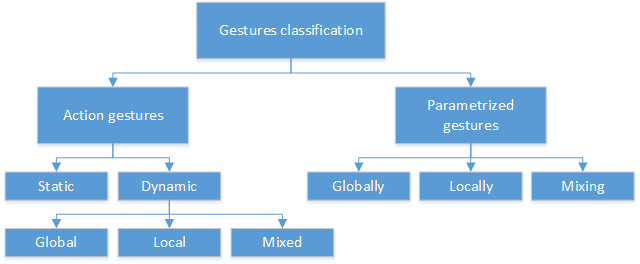
\includegraphics[width=0.8\columnwidth]{figures/gestureClassification.png}
 \caption[]{Classification of gestures proposed in the thesis}
 \label{thesisgesturetypes}
\end{figure}

In Section $3.1$ the three main classifications of gestures based on the existing literature have been presented. Particularly important for further research and to properly define the problem of gesture recognition may be the last of the presented taxonomies, which defines a wide range of possible gestures occurring in human-computer interaction.

It should be noticed that the previously mentioned classifications are defined strictly due to the characteristics of individual gestures, which may cause the selection of appropriate gesture recognition methods difficult. Therefore, it was decided to propose a new taxonomy that will be based on previously presented taxonomies \cite{kammer_taxonomy_2010}\cite{Karam05ataxonomy}\cite{AignerTaxonomy} and in addition will be focused on the gesture recognition methods and will be defined strictly in the context of gesture recognition.

The proposed classification involves the following division by conveyed informations:
\begin{itemize}
\item action gestures (1),
\item parametrized gestures (2).
\end{itemize}

The former group (1), represents gestures, which their identification is based only on detection of gesture occurence. This means that action gestures have assigned some meaning, and the occurrence of this type of gesture implies execution of pre-defined action. It should also be noted that gestures of this type do not convey any additional parameters which define or describe the action. An example of this type can be gesture showing open hand, which could mean stop playing music. Another example might be a moving index finger in circles, which means rotating previously selected object of the specified number of degrees.

Gestures, which may be included into a parameterized gestures (2), provide additional parameters related to the context of the gesture. In contrast to previous group, parametrized gestures carry additional meaning or parameters needed to perform the gesture. An example of this kind of gestures might be a similar gesture to the previously mentioned instance of action gestures --- making circles through moving finger --- but in this case --- in addition to returned information about recognized gesture --- a value of angle, which should be used to rotate selected object, is also be conveyed.

Action gestures (1) is divided into static (1.1) and dynamic (1.2). The former group relates to gestures, that are not variable in time, therefore hand posture, its position and rotation are fixed during hand gesture performing. It should also be mentioned that these gestures should be independent of the orientation relative to the environment and the occurrence of this gesture is detected only on the basis of hand posture.

Dynamic action gestures (1.2) refer to the group of gestures which are constant and non-parametrized variable over time in terms of hand posture, position and rotation in space. This group is further divided into global, local and mixed. Global were detected based on a fixed hand posture and specified movement, which may relate both to changes in position and rotation. In the case of local, hand posture is only variable in time, while the mixed include gestures, for which both the hand posture, as well as the position and rotation vary with time. 

For parameterized gestures (2) division of locally (1.1), globally (1.2) and mixed parameterized gestures is distinguished. Globally parameterized gestures include gestures, whose parameters are determined by values of position and rotation or its changes of the hand. For instance, swipe gesture can be considered as globally parametrized gesture, where the parameter is the length of the swipe motion. Recognition of globally parametrized gestures is performed on the basis of unchanging hand posture or specific changes in the shape of the hand posture over time.

Locally parameterized gestures (1.2) include gestures whose the hand posture or its changes are parameterized, for example a distance between index finger and thumb of one hand may be a parameter for scaling gesture. Gestures of this kind should be independent of the position and rotation in space. Recognition should be based on the hand posture, which can be problematic when it will be time-varying.

Mixed parametrized group (1.3) represents gestures which both
\begin{itemize}
\item hand posture or hand posture changes over time,
\item and hand posture values or changes of position and rotation
\end{itemize}
are parametrized. Gestures of this group are recognized based on hand posture.
Classification presented above relates to the previously described taxonomy proposed by Aigner et al. at follows:
\begin{itemize}
\item pointing gestures -- represented by mixed parametrized gestures,
\item static semaphoric -- represented by static action gestures,
\item dynamic and stroke semaphoric -- represented by dynamic action gestures,
\item static iconic -- for demonstrating the shapes of objects represented by static action gestures and for presenting the size of object by locally parametrized gestures,
\item dynamic iconic -- mainly represented by dynamic action gestures, but can also be globally parameterized gestures for indicating the size of the objects,
\item pantomimic -- represented mostly by mixed dynamic action gestures, assuming that they are always performed in the same way,
\item manipulation -- represented by all types of parametrized gestures.
\end{itemize}

\section{Gesture data representation}

LeapSDK provides built-in classes representing real--world object seen by the controller. The basic data unit we get from Leap Motion is a Frame. Frame contains objects like Hands and Pointables (Fingers and Tools), described by features directly related real attributes.

Hand is an object representing a regular human hand. It contains Fingers, and is described by three dimensional values, like: position of center of hand, normal vector and direction vector (pointing from the center to the end of fingers). 

Pointables are objects like Fingers or Tools (which are longer and thinner than Fingers). Both are described by the same set of features: position of tip, pointing direction vector, length and width.

\begin{itemize}
	\item Frame:
	\begin{itemize}
		\item Hands (position of center, normal vector, direction vector)
			\begin{itemize}
				\item Pointables: (tip position, pointing direction, length, width)
				\begin{itemize}
					\item Fingers
					\item Tools
				\end{itemize}
			\end{itemize}
	\end{itemize}
\end{itemize}

All positions are expressed in milimeters, relative to position of controller which is always located in the center of the 3D space. Manufacturer claims, that the accuracy of device is about 0.01mm. Experiments shown results better than 0.2mm, using an industrial robot moving an object in controllers' field of view. This is more than enough, as accuracy of positioning human hand is about 0.4mm. \cite{lmAN} 

\section{Additional processing steps} \label{PreprocessingSection}

Stability of images acquired by Leap Motion can vary, which occurs as noise on captured data -- sometimes fingers may flicker, or nonexisting objects appear in view. Those malfunctions happen for a very short period of time, usually less then 5 frames. 

To improve data stability, a simple preprocessing has been created. Its principle is based on median filter -- it uses a window with custom definied size. For a given frame, for every unique finger which have been captured in the the window, algorithm checks if it should be present in current frame, by checking its neighboor frames within defined radius $r$. It counts occurences of a finger ($f_0$) in a neighboorhood and decides:

\begin{itemize}
\item if $f_0 > r$, a finger should appear in that frame
\item otherwise, there should not be a finger
\end{itemize}

If the finger does not exist in current frame and a check indicates it should, its position is calculated using finger positions in two closest frames where that finger appears, using linear interpolation. Otherwise, a finger is simply removed.

Using data preprocessing causes delay in data transmission to processing threads, proportional $r+1$. For example, while capturing with 50 frames per second, with window radius $r=4$, the delay would be:

$$ \frac{r+1}{fps} = \frac{5}{50} = 0.1 second $$

\chapter{Static gestures recognition}

As was already mentioned, the gestures that can be detected can be divided into two main groups: static gestures and dynamic gestures.
The static gestures can be understood as a chosen position and orientation of fingers and a hand in a single moment, while dynamic gestures are defined as a movement of the hand and fingers in time. 
The problem of static gesture recognition is a subject of following chapter. 
Firstly, the proposed approach is presented, followed by the introduction to the evaluation scheme. 
In last section, the performed experiments are described, which were used to examine the effectiveness of proposed approach.

\section{Proposed methods}

The static gesture recognition problem can be stated as a problem invariant to time.
That means that for each detected hand, the position and orientation can be treated as a new data, uncorrelated to previously classified hands.
With this assumption, one can easily generate multiple samples from the sensors in short time, but it also gives an opportunity to look at the static gesture recognition problem as a problem of classification.

In literature, most of the approaches uses two-dimensional representation of gestures, which makes recognition problems relatively simple and therefore allow to use simple classification algorithms e.g. k-NNs [Gesture recognition toolbox]. 
The three-dimensional representation of data is more complicated to model by the set of features and finally successfully label.
While dealing with 3D data, the position and orientation of hand can be easily affected by the height of the hand above the sensor or a small change in the orientation of the hand with respect to the sensor's coordinate system. 
All of those distortions should not prevent the system from recognizing those gestures as the one as they are similar.
To meet those requirement, it is needed to define what is the ``small'' change in orientation resulting in treating the static gestures as the same one.

\begin{figure}[htb]
\centering
 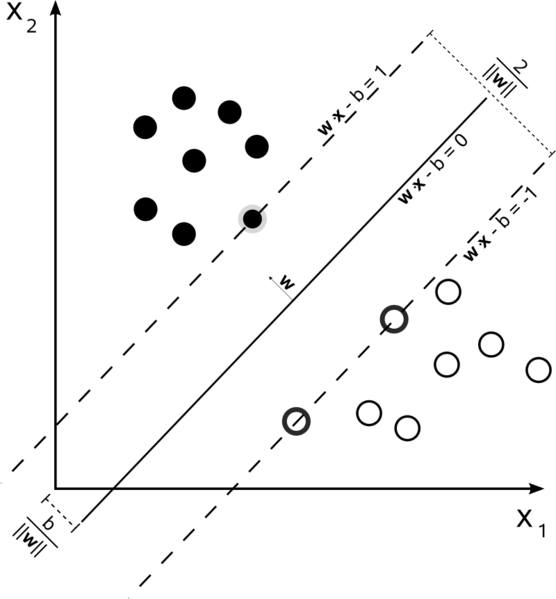
\includegraphics[width=0.6\columnwidth]{figures/SVM.png}
 \caption[]{SVM is a classification algorithm looking for the hyperplane that maximizes the margin between classes\footnotemark}
 \label{svmmargin}
\end{figure}

In application of the library presented in this thesis, it is assumed that the learning process can be done offline, while strict online requirements has to be met in the recognition part. 

To meet listed requirements, the Support Vector Machines (SVMs)\cite{Cortes:SVM} were used as a robust classification algorithm.
The SVMs were chosen as there exist a solid mathematical background supporting the simple idea of maximizing the margin between classes.
Moreover, the SVMs were chosen due to the popularity in the current research trends and is commonly used technique in biology, robotics or IT for solving data classification problems.
The another advantage is the existence of the open-source library libSVM \cite{libSVM}, which contains the implementation of the SVM in different programming languages.
In the original work, SVMs were designed to be only to classify between two classes, but the idea was expanded to utilize the one-vs-all classification allowing to differentiate between multiple classes.
This might be the drawback, as the for $n$ classes, it is necessary to train $n$ SVMs each to classify one class against all samples from the rest of the classes. 
The efficiency of SVMs depends on correctly choosing the kernel function used to map the separation problem into higher dimension with expectation to achieve a classification problem that can be separated.
There exists several kernel functions:
\begin{itemize}
\item linear: $K(x_i, x_j) = x_i^Tx_j$.
\item polynomial: $K(x_i, x_j) = (\gamma x_i^Tx_j + r)^d, \gamma > 0$.
\item radial basis function (RBF): $K(x_i, x_j) = exp(-\gamma ||x_i - x_j||^2), \gamma > 0$.
\item sigmoid: $K(x_i, x_j) = tanh(\gamma x_i^Tx_j+r)$.
\end{itemize}
where $\gamma$, $r$, and $d$ are kernel parameters. 
According to the authors of the library \cite{libSVM}, linear kernels perform the best, when used for linearly separable problems, while RBF kernels are the most versatile ones and are recommended for most of the applications.

\footnotetext{\url{http://en.wikipedia.org/wiki/File:Svm_max_sep_hyperplane_with_margin.png}}

The problem of classification assumes that each sample consists of set of features, which describe a sample and can be used to distinguish it from the other samples.
Additionally, each sample has a known or unknown label, which define the membership of the sample to the classification class. 
The samples with the known labels can be used to train the classification system.
Trained classification system is used to predict the labels for the provided samples.

In application of gesture recognition the classification be divided into two flows: the training part (offline) and the recognition part (online). 
The static gesture processing flow is presented at fig.~\ref{staticsol}.
In training part, the library will be provided with the recorded samples of static gestures with known correspondences to the static gesture classes. 
From those samples, the sets of features are computed, which are used to train the classifier.
The recognition part assumes to have trained classifier. 
The recognition part is provided with samples of static gestures without labels. 
For each sample the sets of features are computed and then given as input to the trained classifier.
The classifier provides the information of the predicted gesture's class membership (label) for each input sample.

\begin{figure}[htb]
\centering
 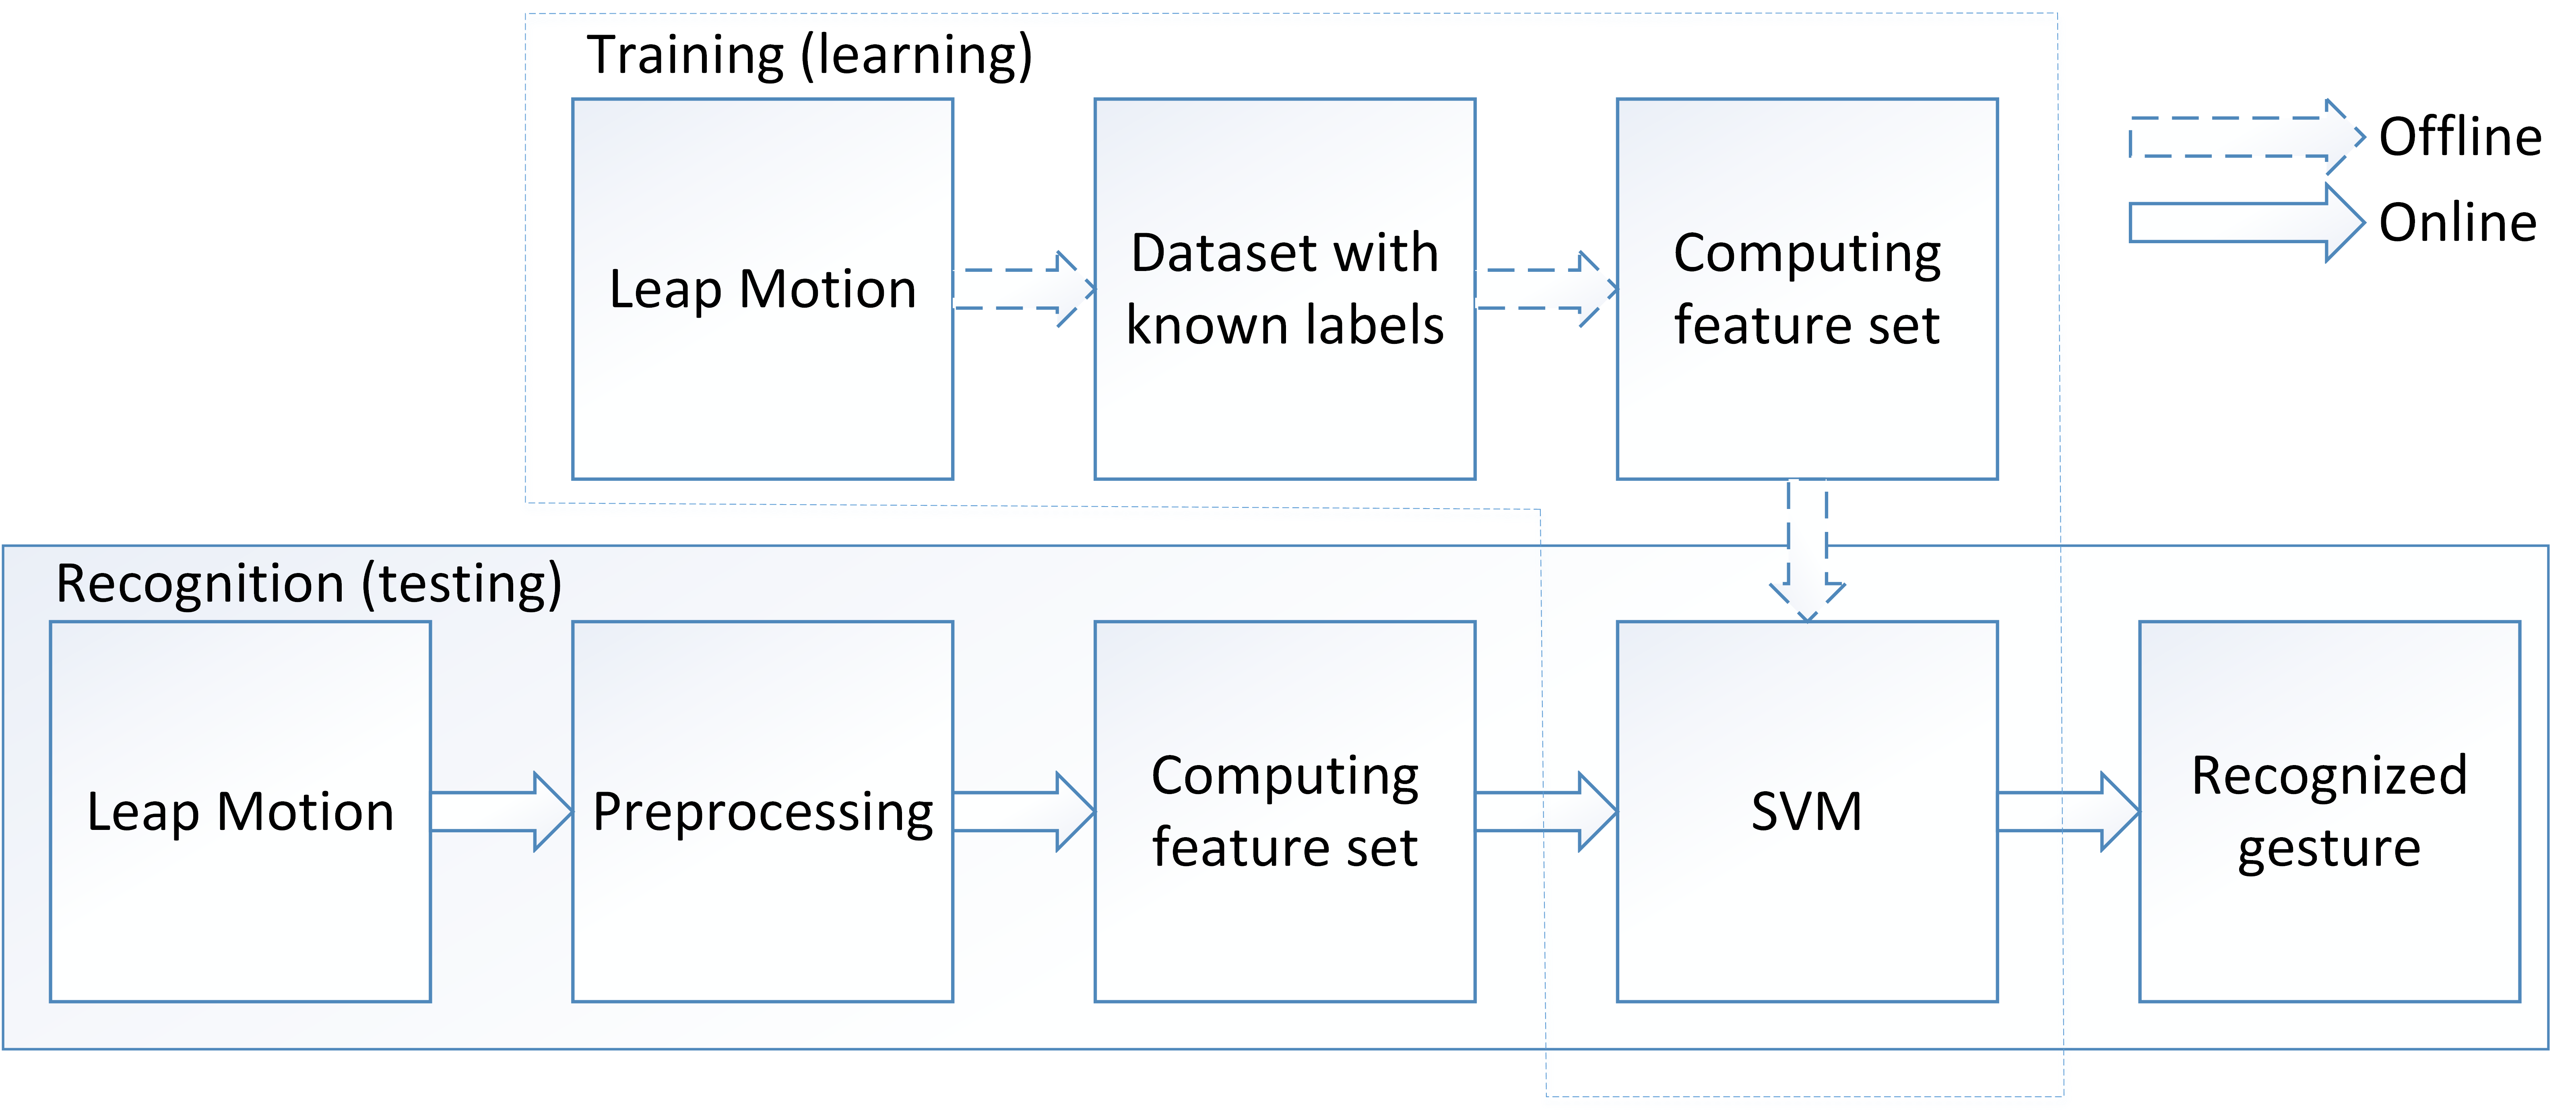
\includegraphics[width=1\columnwidth]{figures/StaticGestures.png}
 \caption[]{Proposed solution blocks for learning and recognition parts of static gestures recognition problem}
 \label{staticsol}
\end{figure}

While presented approach can be treated as state-of-the-art approach it still cannot be used without defining proper feature sets for gesture recognition.
The naive solution would be to use the raw data from Leap motion sensor as the feature set.
This solution was tested, but provided poor results as the proposed features were dependent on the position, orientation and scale of hand. 
Even small movement in any direction meant problems with stable recognition. 
The theoretical literature suggests to compute a set of features invariant to wanted transformations, which can allow to fully distinguish between different classes.
The proposed feature sets are application dependant.
Together the fact that the gesture recognition using the data similar to the data provided by the Leap Motion sensor has not been yet examined by the researches meant that seeking right feature set is a task of the thesis.
The task is undertaken in experimental section~\ref{static:exp}.

\section{Evaluation methodology}

\subsection{Assumptions}
To provide user with library working in different conditions, it was assumed that the gesture is treated as the same one independently with respect to the translation, rotation and scale of the hand. 
This assumption means that the static gesture rotated by unknown angles, translated in sensor coordinate system and also with different hand sizes should still be recognized as the same gesture.
Invariance to the rotation, translation and scale poses a great challenge to the recognition, but allows the future users of API to fully utilize the feasibility of the library.
It is worth mentioning that, it does not reduce the possible applications of the library, as an assignment of static gesture to already defined class allows to find the transformation between the model of the class and observed gesture.
And further, this transformation can be used to examine the parameters of the instance of the model e.g. rotation of the hand.

\subsection{Recorded datasets}

To propose and test the quality of the features twelve static gestures were chosen:
\begin{enumerate}
\item the peace sign,
\item a fist,
\item full hand with space between each finger,
\item from American Sign Language: ``I love you'' sign,
\item sign ``gun'' created by putting thumb and forefinger up, while holding the rest fingers in a fist,
\item all fingers in a fist with exception of thumb, which is up,
\item the sign X made with the forefingers of both hands,
\item the sing ``Time'' used e.g. by coaches in basketball games.
\item sign simulating rotating a knob by two fingers,
\item sign simulating rotating a knob by five fingers.
\end{enumerate} 

\begin{figure}[htb]
\centering
 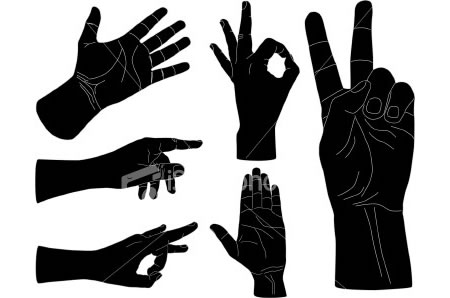
\includegraphics[width=1.0\columnwidth]{figures/static_gestures.png}
 \caption{Recorded static gestures used for evaulation}
 \label{staticgesturesdata}
\end{figure}
The gestures are also presented at fig.~\ref{staticgesturesdata}.

The sample data of each gestures were recorded using the continuous mode of recording, while moving the hands in different directions and changing the orientation of the hands.
The hands were moved and rotated as each repeated static gesture is always a little bit different from the previously recorded samples/ 
For each of the proposed gestures, each author of this thesis recorded approximately 1000 samples.

Having samples with known labels, the whole dataset was separated into training and testing sets in relation $2:1$. 
For the training, the k-fold cross-validation (CV) scheme was used, which searches for optimal $C$ and $\gamma$ parameters of SVM trying to train the classification algorithm while preventing the algorithm from over-fitting the training data.
This method is used to find the optimal parameters of the classification system, while estimating the performance is done on the data not used in the training part. 
In standard version of the CV, the gathered data is divided into two sets: one containing $k-1$ parts of the data, the other $1$ part of the data. 
The first is used to train the classification system, while the rest of the gathered data is used to estimate how well the system is learnt.
In the next iteration, the CV parts are shuffled by still having the ratio of training and validation sets.
After the training, the final performance is estimated by calculating the percent of correctly recognized labels to the total size of the testing set known as recognition rate.


\section{Experiments}
\label{static:exp}

Firstly, the experiments to find the proper set of features were conducted. The first proposed vector of features consisted of:
\begin{itemize}
\item number of fingers in frame,
\item the euclidean distance between consecutive finger's tips,
\item the absolute angles between consecutive fingers.
\end{itemize} 

This feature set did not take into account the relative position of fingers to the hand.
The second feature set is a first feature set extended by the distances between consecutive finger tips and the position of the hand's palm.
The third feature set contains features from second feature set extended by the five angles between fingers and normal of hand's palm.
Those, 3 proposed feature sets were firstly tested on all $10$ recorded.
The firstly tested set of all static gestures contained gestures, which were undistinguishable for the Leap Motion, because they did not take into account the way how the Leap Motion works. 
For gestures like fist or 'X' the recorded data contained almost no information how to classify those gestures.
That's why the experiments were repeated on the five gestures, which could be easily distinguish using the data provided by Leap Motion. 
For this experiment the gestures peace, hand, ''I love you'', fist with thump up and rotating knob by 5 fingers were chosen.
The results achieved by those methods are presented in the table~\ref{staticfeat}.

\begin{table}[htp!]
	\label{staticfeat}
	\caption{Results obtained by experimental feature sets by the libSVM library}
    \begin{tabular}{|c|c|c|c|c|}
    \hline
    ~                                                   & $5$ gestures, CV & $5$ gestures, test set & $10$ gestures, CV  & $10$ gestures, test set \\ \hline
    feature set $1$                     & $87.072\%$ & $87.943\%$ & $69.987\%$ & $68.422\%$   \\ \hline
    feature set $2$                     & $87.072\%$ & $87.943\%$ & $69.987\%$ & $68.422\%$          \\ \hline
    feature set $3$                     & $87.072\%$ & $87.943\%$ & $69.987\%$ & $68.422\%$           \\ \hline
    feature set $4$                     & $81.150\%$ & $80.998\%$ & $68.438\%$ & $68.630\%$          \\ \hline
    feature set $5$                     & $86.544\%$ & $85.075\%$ & $77.101\%$ & $77.518\%$          \\ \hline
    feature set $6$                     & $92.762\%$ & $93.096\%$ & $80.543\%$ & $81.235\%$           \\ \hline
    \end{tabular}
\end{table}

For problem of recognition of $5$gestures, three first feature sets resulted in over $87\%$ recognition rate on testing sets, which was believed to be a good result.
The same tests for problem of recognition of $10$ gestures resulted in lower recognition rates.
For feature sets $1-3$ the recognition rate was below $70\%$, which could be unsatisfying from the perspective of the purpose of the application.
The low recognition rate was analysed and revealed that the fingers are numbered accordingly to the position in Z axis of the tip of the finger.
This means that when finger's tips are approximately on the same position in Z axis, the numbering can change rapidly and proposed features are compared between different fingers.
To achieve features that would be invariant to the numbering of the fingers, the feature set was slightly modified.
Instead of containing the absolute angles and distances between consecutive fingers, it was proposed to contain the five greatest values of angles and five greatest values of distances between all combinations of finger pairings.
The same sorting approach was used for the angles and distances between fingers and hand's palm.
The feature sets $1$, $2$, $3$ with sorting scheme were respectively called feature sets $4$, $5$, $6$.
Again, the same dataset with $5$ and $10$ gestures was used to evaluate those methods. 
The results are yet again presented in table~\ref{staticfeat}.
This approach was tested on the same training set and allowed to increase the recognition rate.
The best results in both tasks were achieved in case of feature sets $6$.
The simple alleviation of finger numbering problem allowed to top the previous results with recognition rates $93.096\%$ for $5$ gesture problem and $81.235\%$ for $10$ gesture problem. 

\begin{table}[htp!]
\begin{center}
	\label{staticfeatlin}
	\caption{Results obtained by experimental feature sets by the libLinear library}
    \begin{tabular}{|c|c|c|c|c|}
    \hline
    ~                                                   & $5$ gestures, CV & $5$ gestures, test set & $10$ gestures, CV  & $10$ gestures, test set \\ \hline
    feature set $1$                     & $78.282\%$ & $78.283\%$  & $50.596\%$ & $50.593\%$ \\ \hline
    feature set $2$                     & $78.282\%$ & $78.283\%$  & $50.596\%$ & $50.593\%$ \\ \hline
    feature set $3$                     & $78.282\%$ & $78.283\%$  & $50.596\%$ & $50.593\%$ \\ \hline
    feature set $4$                     & $78.205\%$ & $78.242\%$  & $50.658\%$ & $50.575\%$ \\ \hline
    feature set $5$                     & $79.527\%$ & $79.502\%$  & $55.284\%$ & $55.263\%$ \\ \hline
    feature set $6$                     & $88.076\%$ & $88.138\%$  & $64.747\%$ & $64.830\%$ \\ \hline
    \end{tabular}
    \end{center}
\end{table}

While using more data and longer feature sets usually allows to achieve better results, it is worth to notice the growth of training time of classification technique. 
In case of $5000$ training samples the typical training process of radial SVM took approximately $12$ hours on standard desktop PC. 
This computing time can be unacceptable by the users of the library and the tests with another SVM library, libLinear~\cite{libLinear} were performed. 
The libLinear's implementation of SVM utilizes the linear kernels and is dedicated for the large data training sets with multiple number of features. 
This library reduced the training time to about $5$ seconds.
Again, the same tests as for the libSVM were performed to compare both approaches.
All achieved results are presented in tab.~\ref{staticfeatlin}.
For the 5 gesture case, the libLinear achieved $88.138\%$ on testing set while using feature set 6 compared to the $93.096\%$ achieved by libSVM in the same condition.
In this case, the libLinear might be good choice as the recognition rate is lower by about $5\%$.
For 10 gesture case, libLinear achieved $64.830\%$ compared to $81.235\%$ by LibSVM, which is a significantly lower recognition rate.
It's up to user to decide which library to use, but in most recognition applications, the library can be learnt offline and only used online.
That is why, the authors of the thesis recommend the SVM with RBF kernels for static gesture recognition task.

From the results obtained by the libSVM and libLinear on different feature sets, the feature set $6$ was chosen as the one yielding the best results and used in further analysis.


Another factor, that might have an influence on the results is the preprocessing part, which should allow to partially remove noise from the data and thus increase the recognition rates. 
The preprocessing operates in the window of hands poses recorded over time, which size can be modified. 
The typical library usage allowed to gather data with $60Hz$, while it is assumed that the recognition can be performed with lower framerate. The difference can be efficiently used by defining the appropriate preprocessing window.
For these reason, the experiments with no preprocessing and preprocessing with width size equal to $5$, $10$, $15$, $20$, $30$ were performed and the influence on the recognition rate was examined.
The results are presented in tab.~\ref{staticpre}.
The achieved results confirm the need and importance of proper data preparation in task of data classification.
For gesture recognition task containing $5$ gesture poses, preprocessing allowed to increase the recognition rate from $93.096\%$ to over $99\%$ for window sizes equal or wider than $15$. 
In task of correctly detecting 10 gestures, the preprocessing allowed to increase recognition rate from $81.235\%$ to over $84\%$ for windows sizes equal or wider than $10$.
From those results, the preprocessing width of $10$ was chosen as the one allowing to significantly improve recognition rate in almost any possible application of the library.
The preprocessing of width $10$ was used for all further experiments if not stated otherwise.

\begin{table}[htp!]
\begin{center}
	\label{staticpre}
	\caption{The recognition rate achieved with feature set $6$ and different parameters of preprocessing}
    \begin{tabular}{|c|c|c|c|c|}
    \hline
    preprocessing                                                   & $5$ gestures, CV & $5$ gestures, test set & $10$ gestures, CV  & $10$ gestures, test set \\ \hline
    off                     & $92.762\%$ & $93.096\%$  & $80.543\%$ & $81.235\%$ \\ \hline
    width = $2$               & $95.641\%$ & $96.527\%$  & $82.736\%$ & $83.172\%$ \\ \hline
    width = $5$               & $95.861\%$ & $96.650\%$  & $83.078\%$ & $83.565\%$ \\ \hline
    width = $10$              & $98.796\%$ & $98.965\%$  & $83.602\%$ & $84.071\%$ \\ \hline
    width = $15$              & $98.981\%$ & $99.150\%$  & $84.112\%$ & $84.494\%$ \\ \hline
    width = $20$              & $99.104\%$ & $99.242\%$  & $84.329\%$ & $84.834\%$ \\ \hline
    width = $30$              & $99.232\%$ & $99.385\%$  & $84.848\%$ & $85.320\%$ \\ \hline
    \end{tabular}
    \end{center}
\end{table}

All of already presented experiments, treated the classification results of consecutive hand poses as time-independent and not correlated with each other.
In real applications, it can safely assumed that the consecutively detected hands are similar to each other and probably define the same gesture.
The remaining question to be answered was the impact of combining the consecutive recognition results for the total recognition percentage.
Firstly, it is important to use not only the class labels for tested dataset, but the whole information provided by SVM containing the measure of classification rate to all possible classes.
This data can be combined to measure the membership rate for each class in a window of set width.
Then the predicted class is the class with maximal measure.
Formally, when there is a need to classify between $k$ classes, the result for $i$-th data in dataset can be represented as:
\begin {equation}
l(i) = [l_{i1}, l_{i2}, ..., l_{ik}]
\end{equation}
where $l_{ik}$ is the likelihood of belonging of $i$-th data to the $k$-th class.
Then combining in a window of width $w$ can be written as:
\begin{equation}
r(i,w) = \sum_{j=i-w}^{i}{ l(j) }
\end{equation}
where the sum of vectors $l$ can be defined freely.
The recognized label is the number of the vector component with the highest value:
\begin{equation}
\mathrm{label} = \argmax_{k}{\{r(i,w)_k\}}
\end{equation}


\begin{figure}[htb]
\centering

\centerline{%
 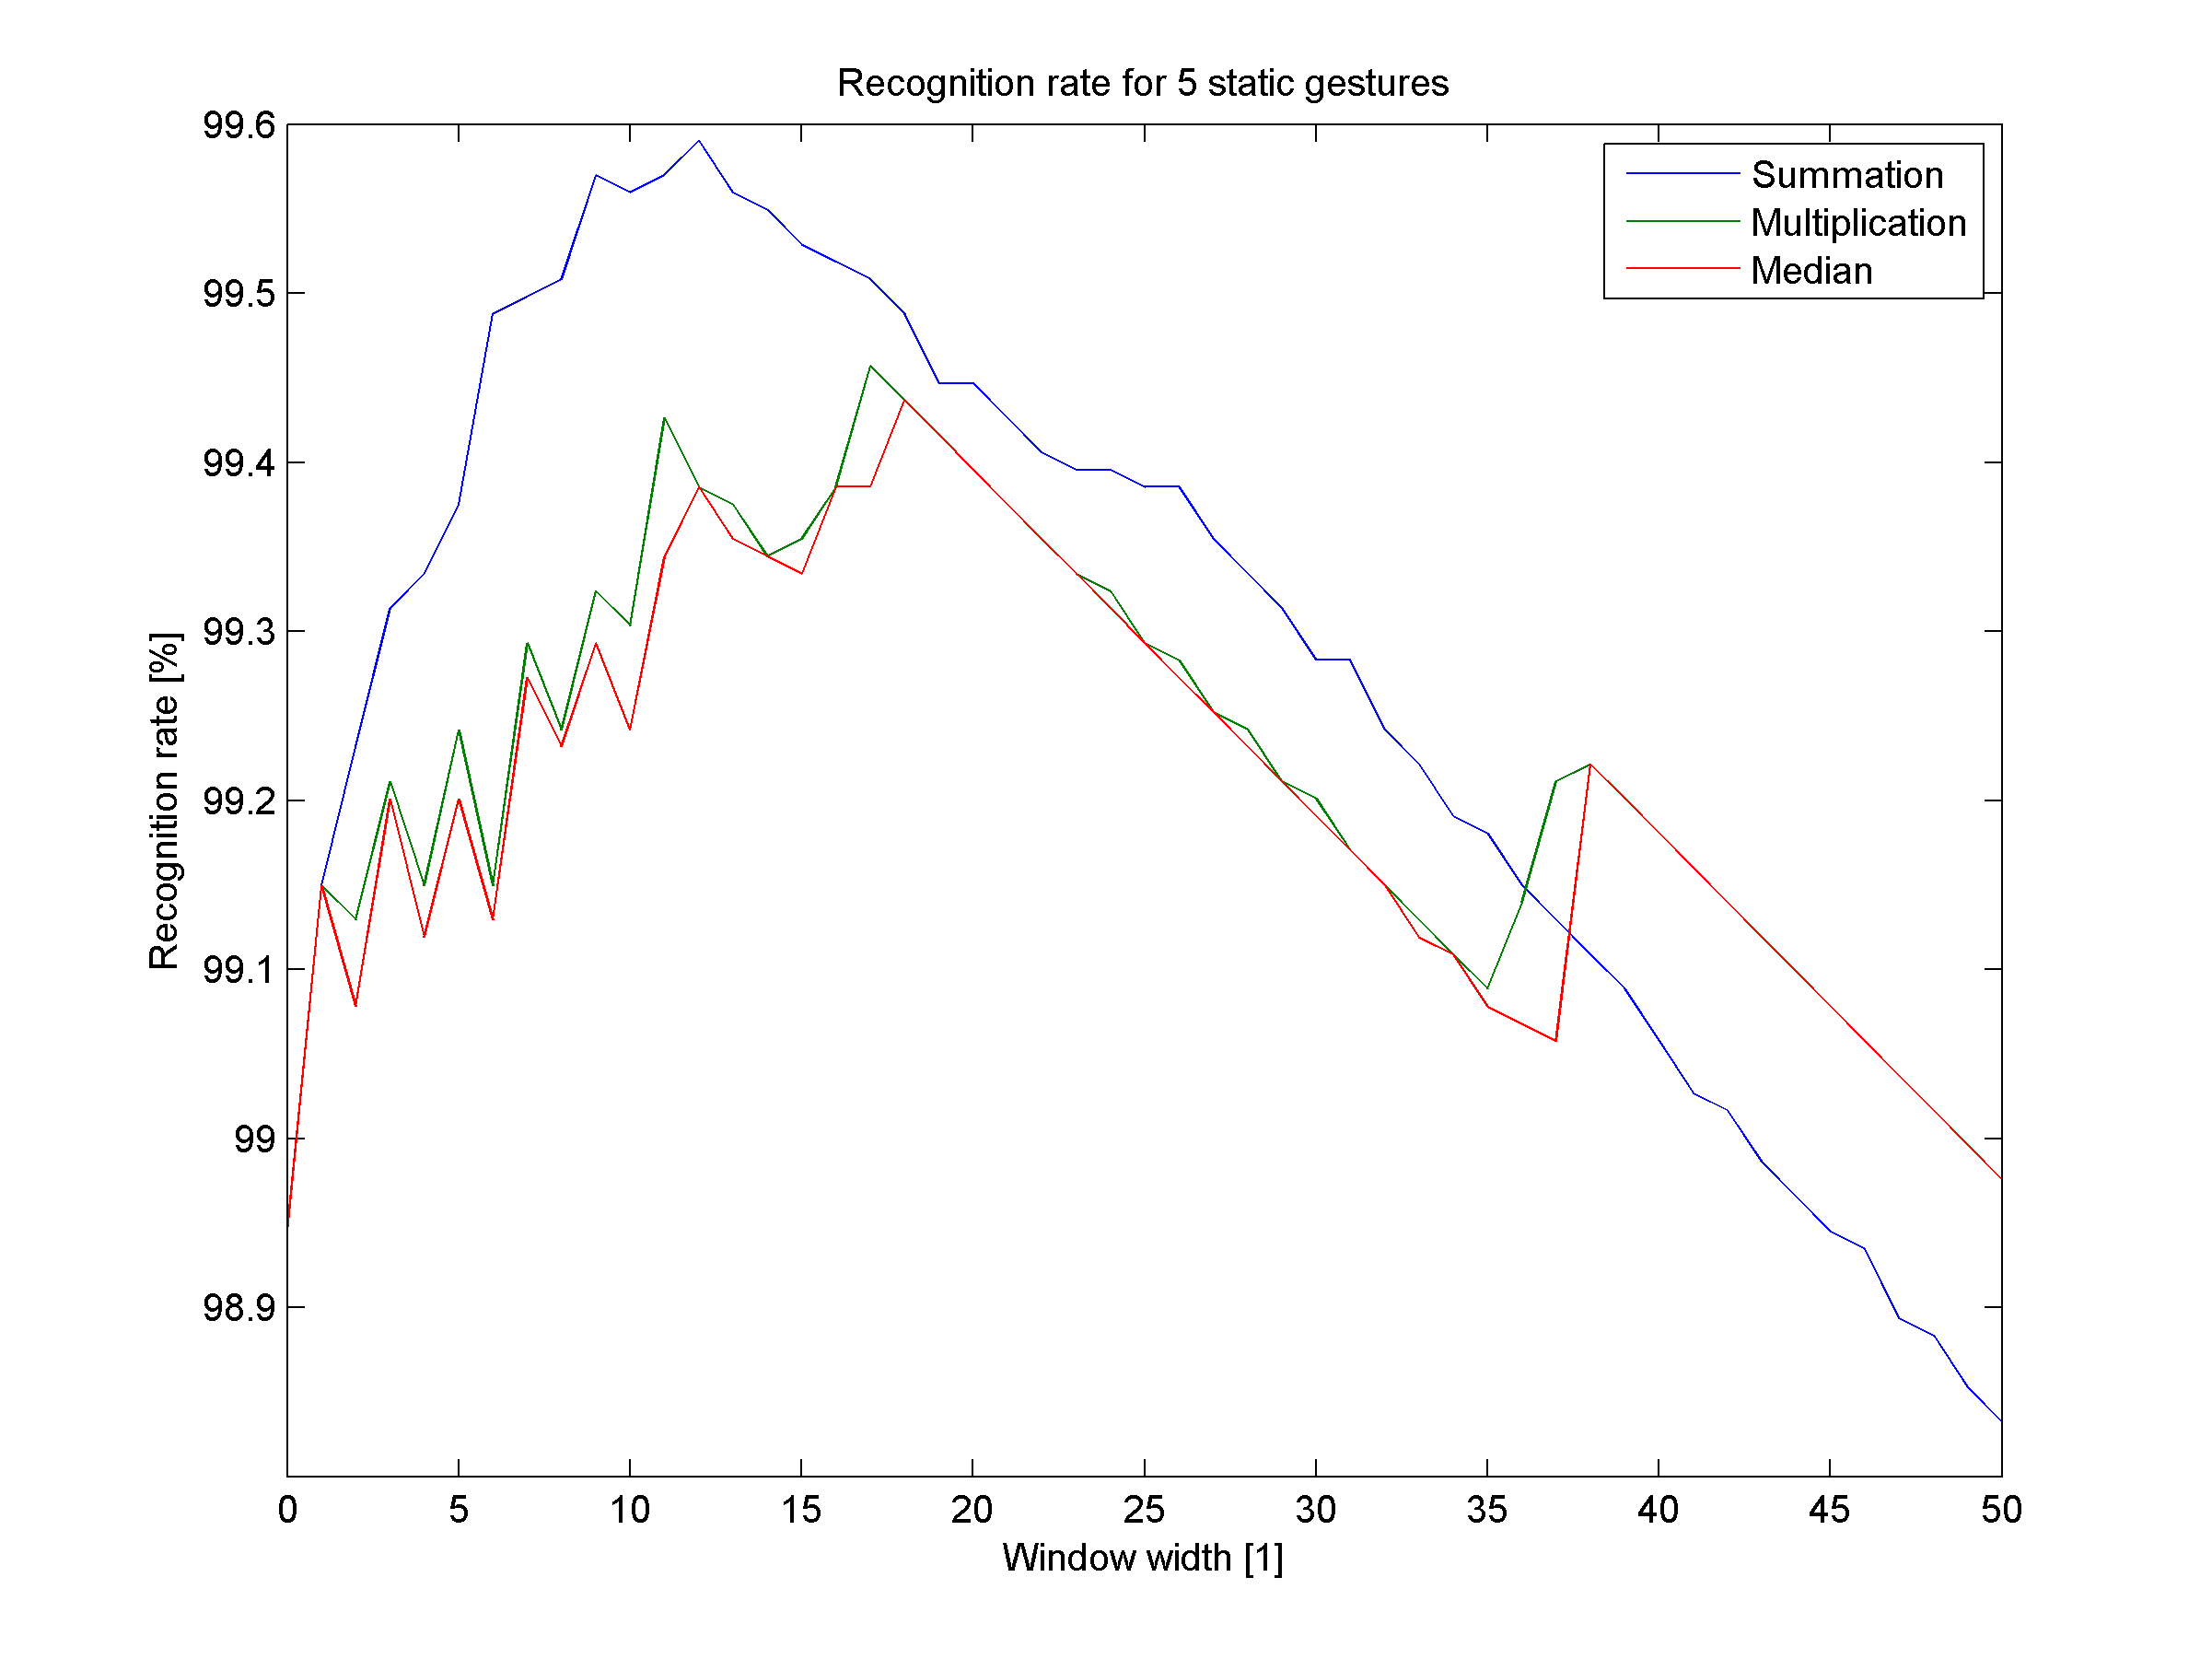
\includegraphics[width=0.5\textwidth]{figures/Mul5.png}
 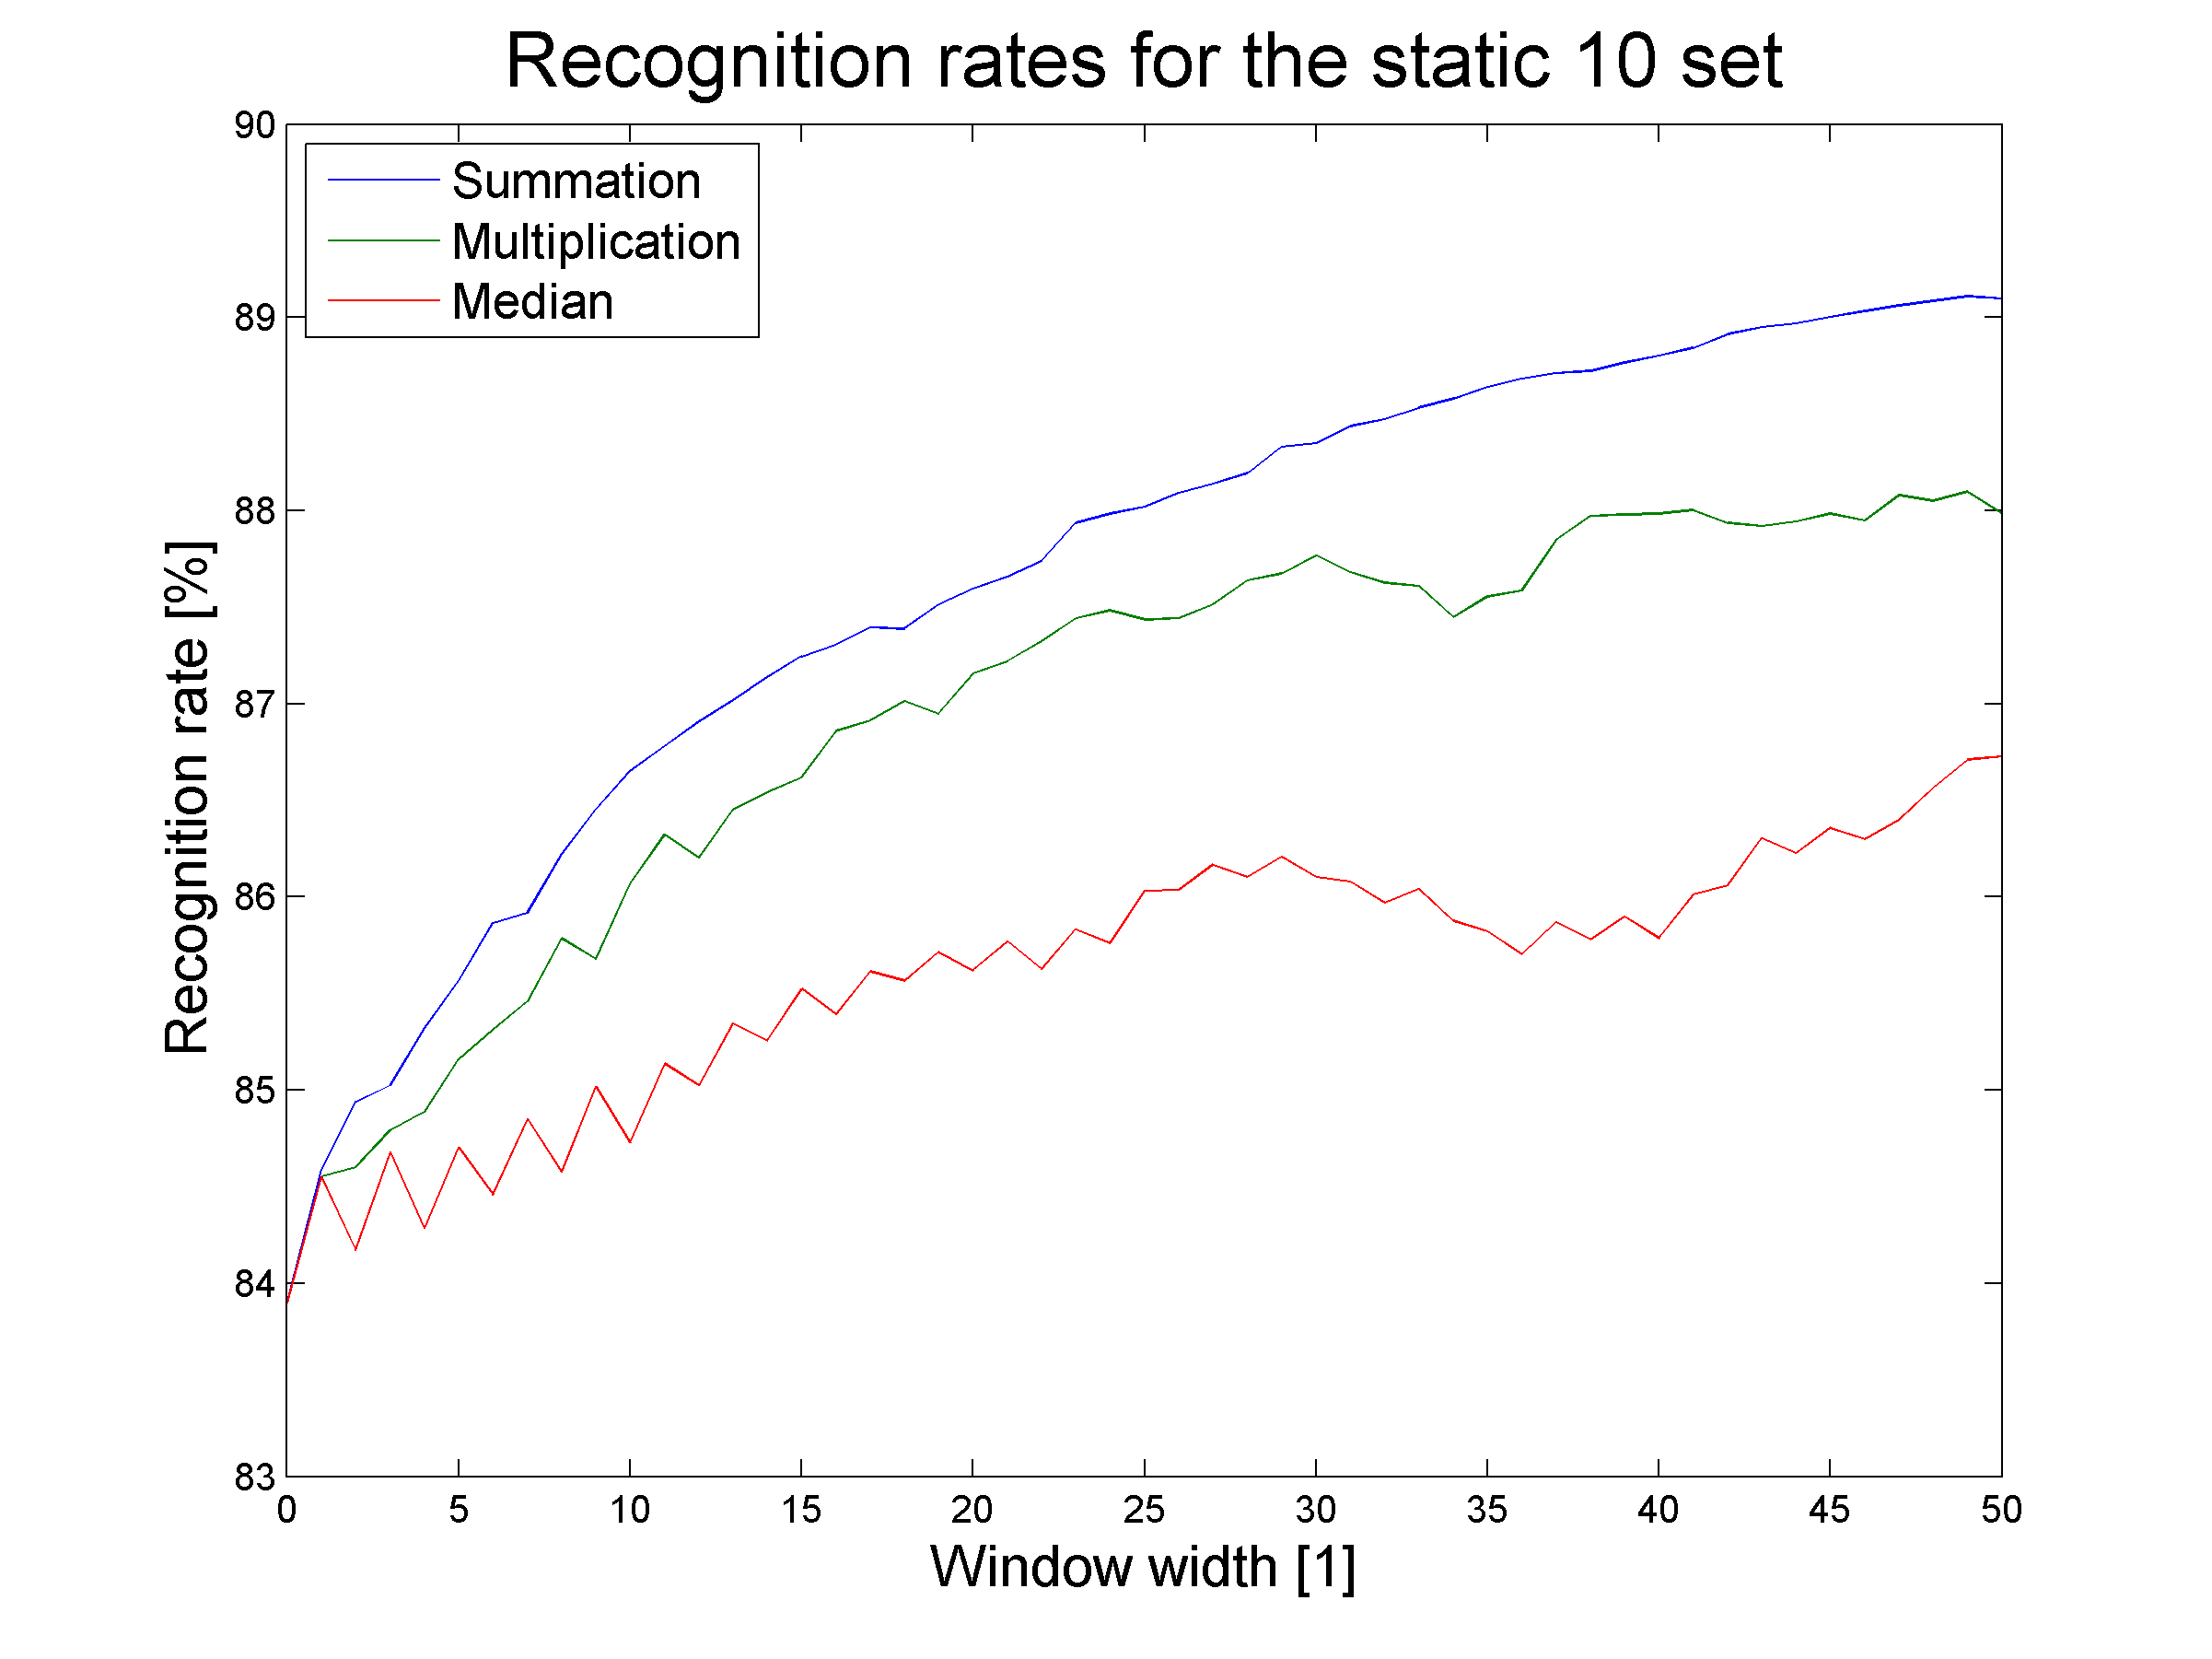
\includegraphics[width=0.5\textwidth]{figures/Mul10.png}
 }%
 \caption{Evaluation of different operators for result combining in case of different window sizes}
 \label{staticoper}
\end{figure}

 

The first approach to defining the sum operator is the operator of simple adding the elements of vectors $l$.
The second proposition is to multiple the corresponding elements of vectors $l$. 
The third approach utilizes the idea of calculating the median elements of vectors $l$.
The three approaches were compared for feature set 6, with preprocessing width equal to 10 for 5 and 10 gestures already used in previous experiments.
Simultaneously, the test were performed for different widths of window and are presented at fig.~\ref{staticoper}.
For almost all possible widths, the summation operator demonstrated the best recognition rate.
For 5 static gesture, the summation with width equal to 10 allowed to achieve the recognition rate over $99.5$\% gaining over $0.5\%$ when compared to solution without postprocessing.
Interestingly, windows wider than 12 resulted in lower recognition rate than the best achieved with window size equal to 10.
For 10 static gesture recognition problem, using window of size equal to 50 allowed to increase the recognition rate by over $5\%$ to the value over $89$\%.
In this case, wider window resulted in better results. 
Similarly to the preprocessing window size, also in postprocessing too wide window will result in delayed recognition rate of shown gesture.
Also, too wide window may result in worse results.
Therefore, the postprocessing window size of 10-15 is recommended, but it also depends on the application of the library.

With simple summation window, the currently achieved result and the results from the past are equally affecting the recognition result. 
Especially for wider windows, it can be assumed that the current measurement is more important than the measurement from the distant past.
That is why, the idea of weighted sum was introduced.
The weight distribution should have the highest weight for the current measurement and smaller values for results that were achieved earlier in time.

\begin{figure}[htb]
\centering

\centerline{%
 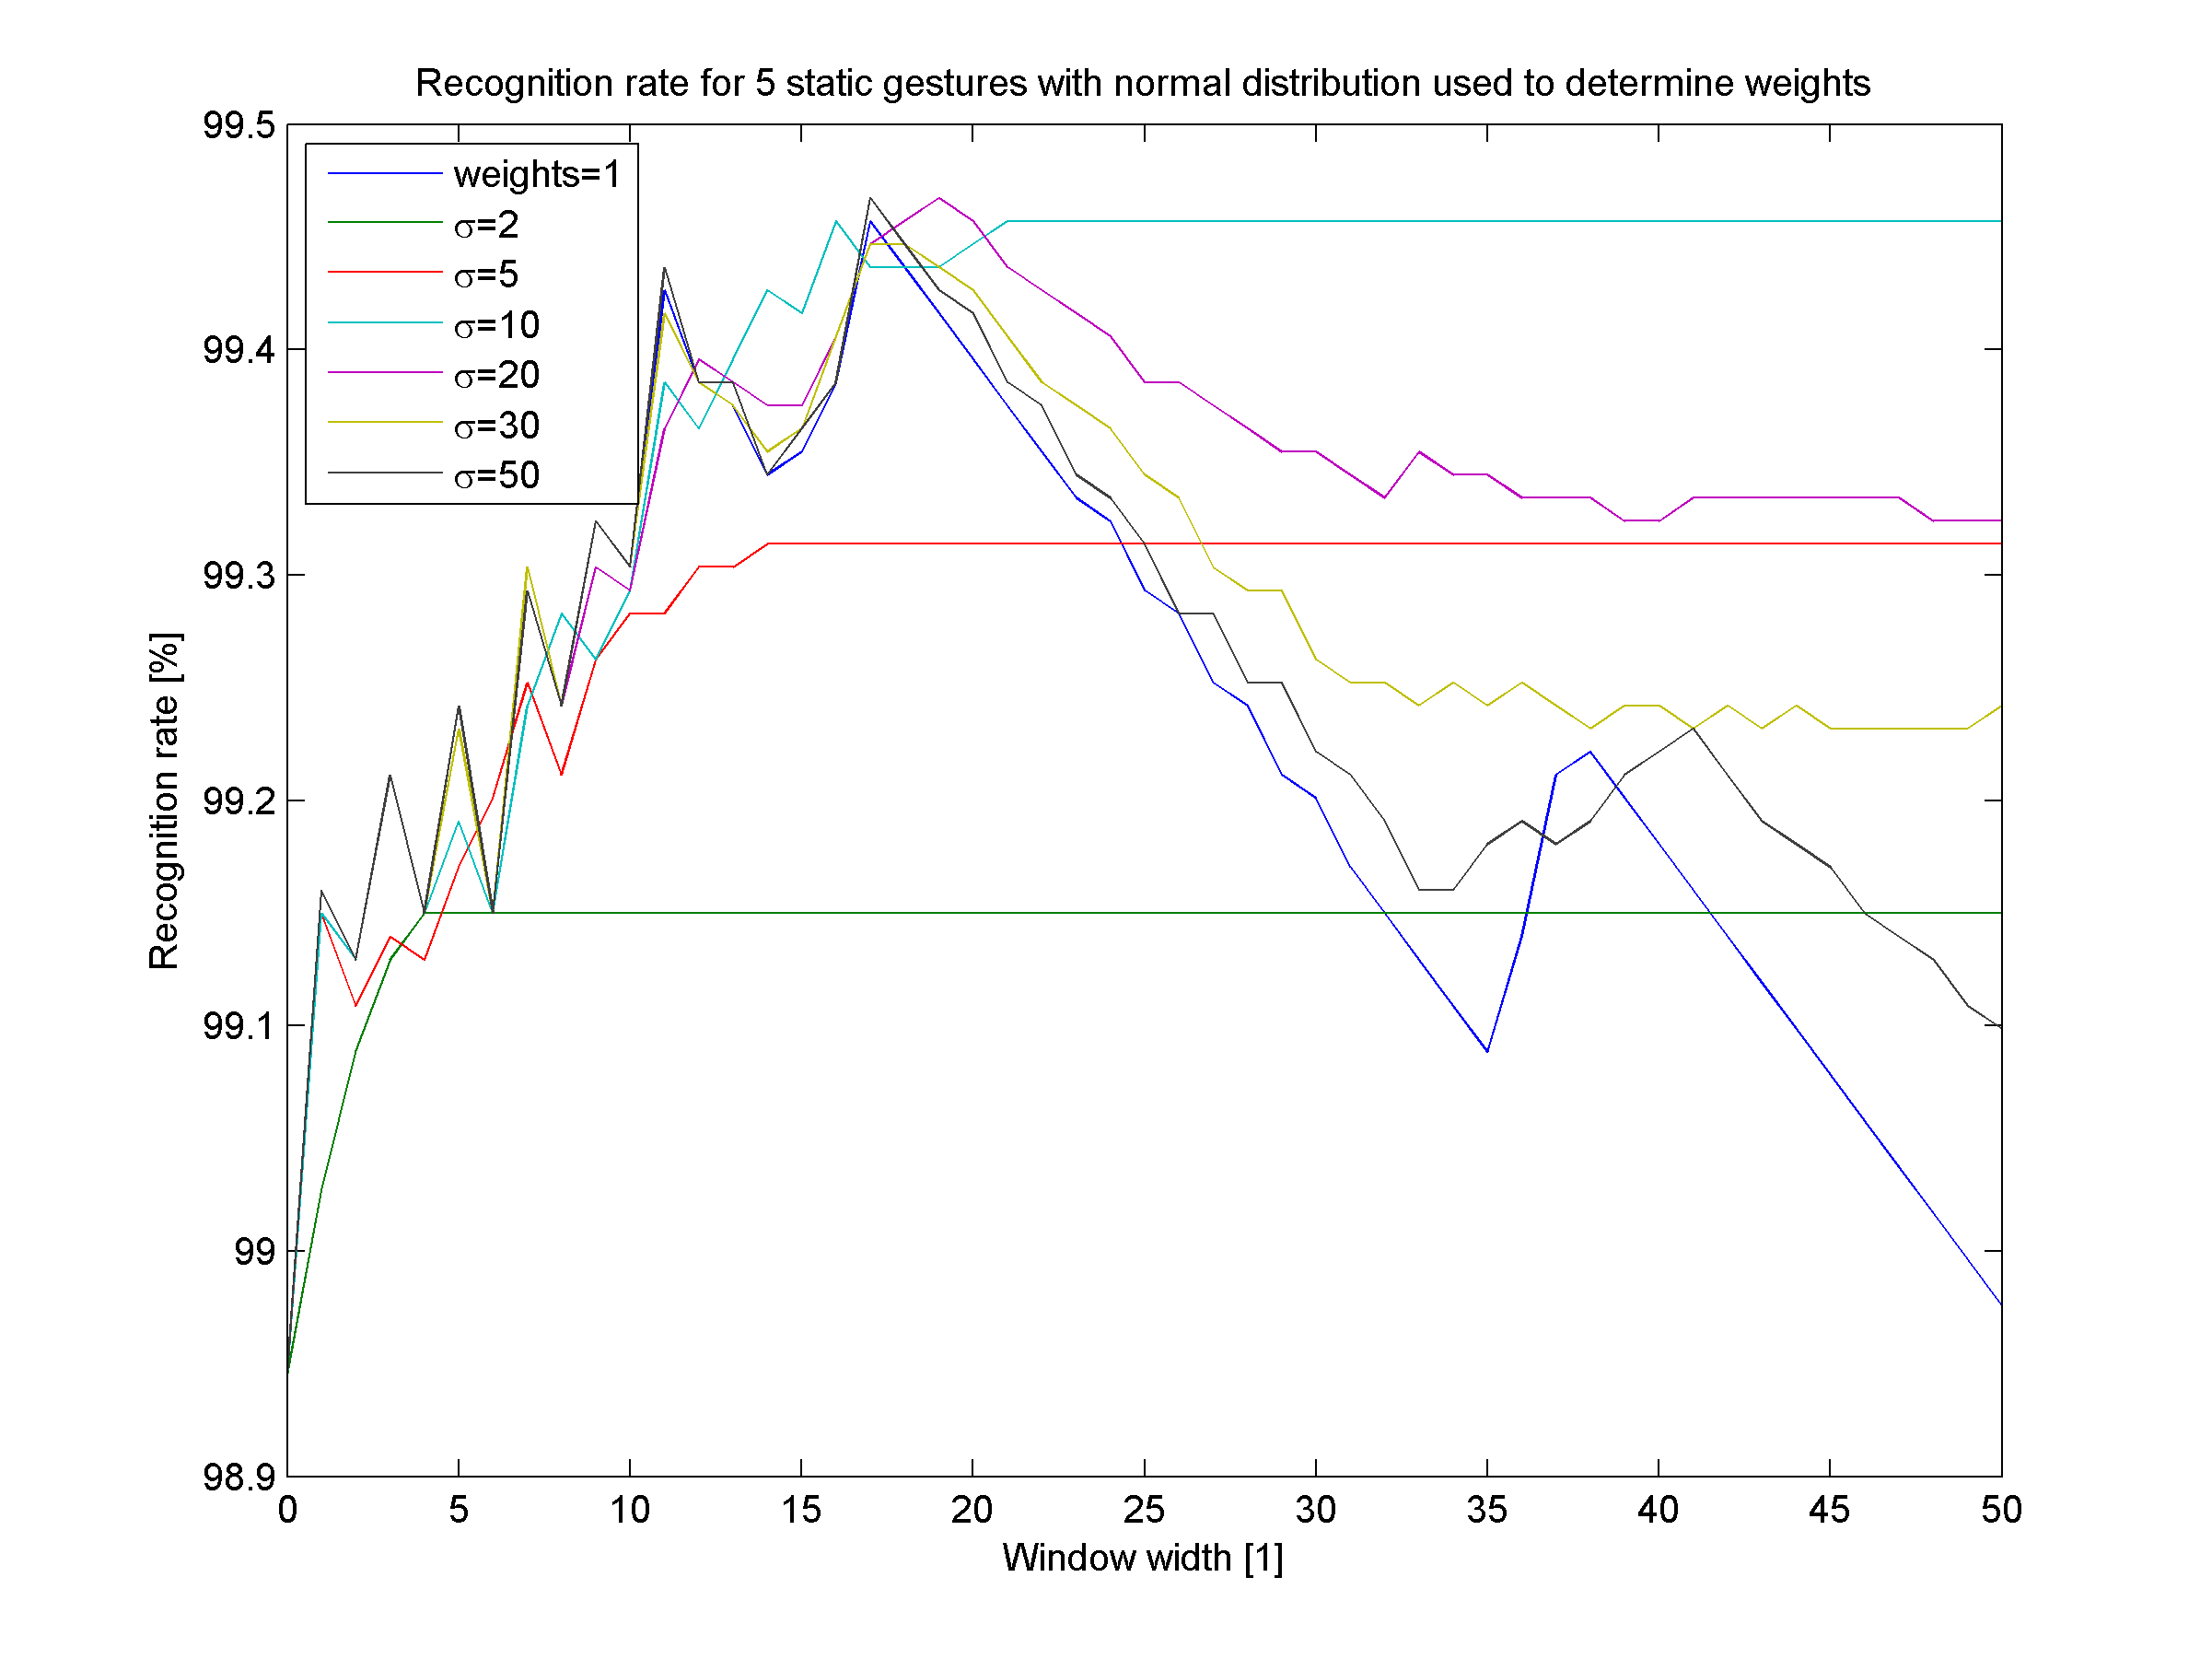
\includegraphics[width=0.5\textwidth]{figures/gaussSum5.png}
 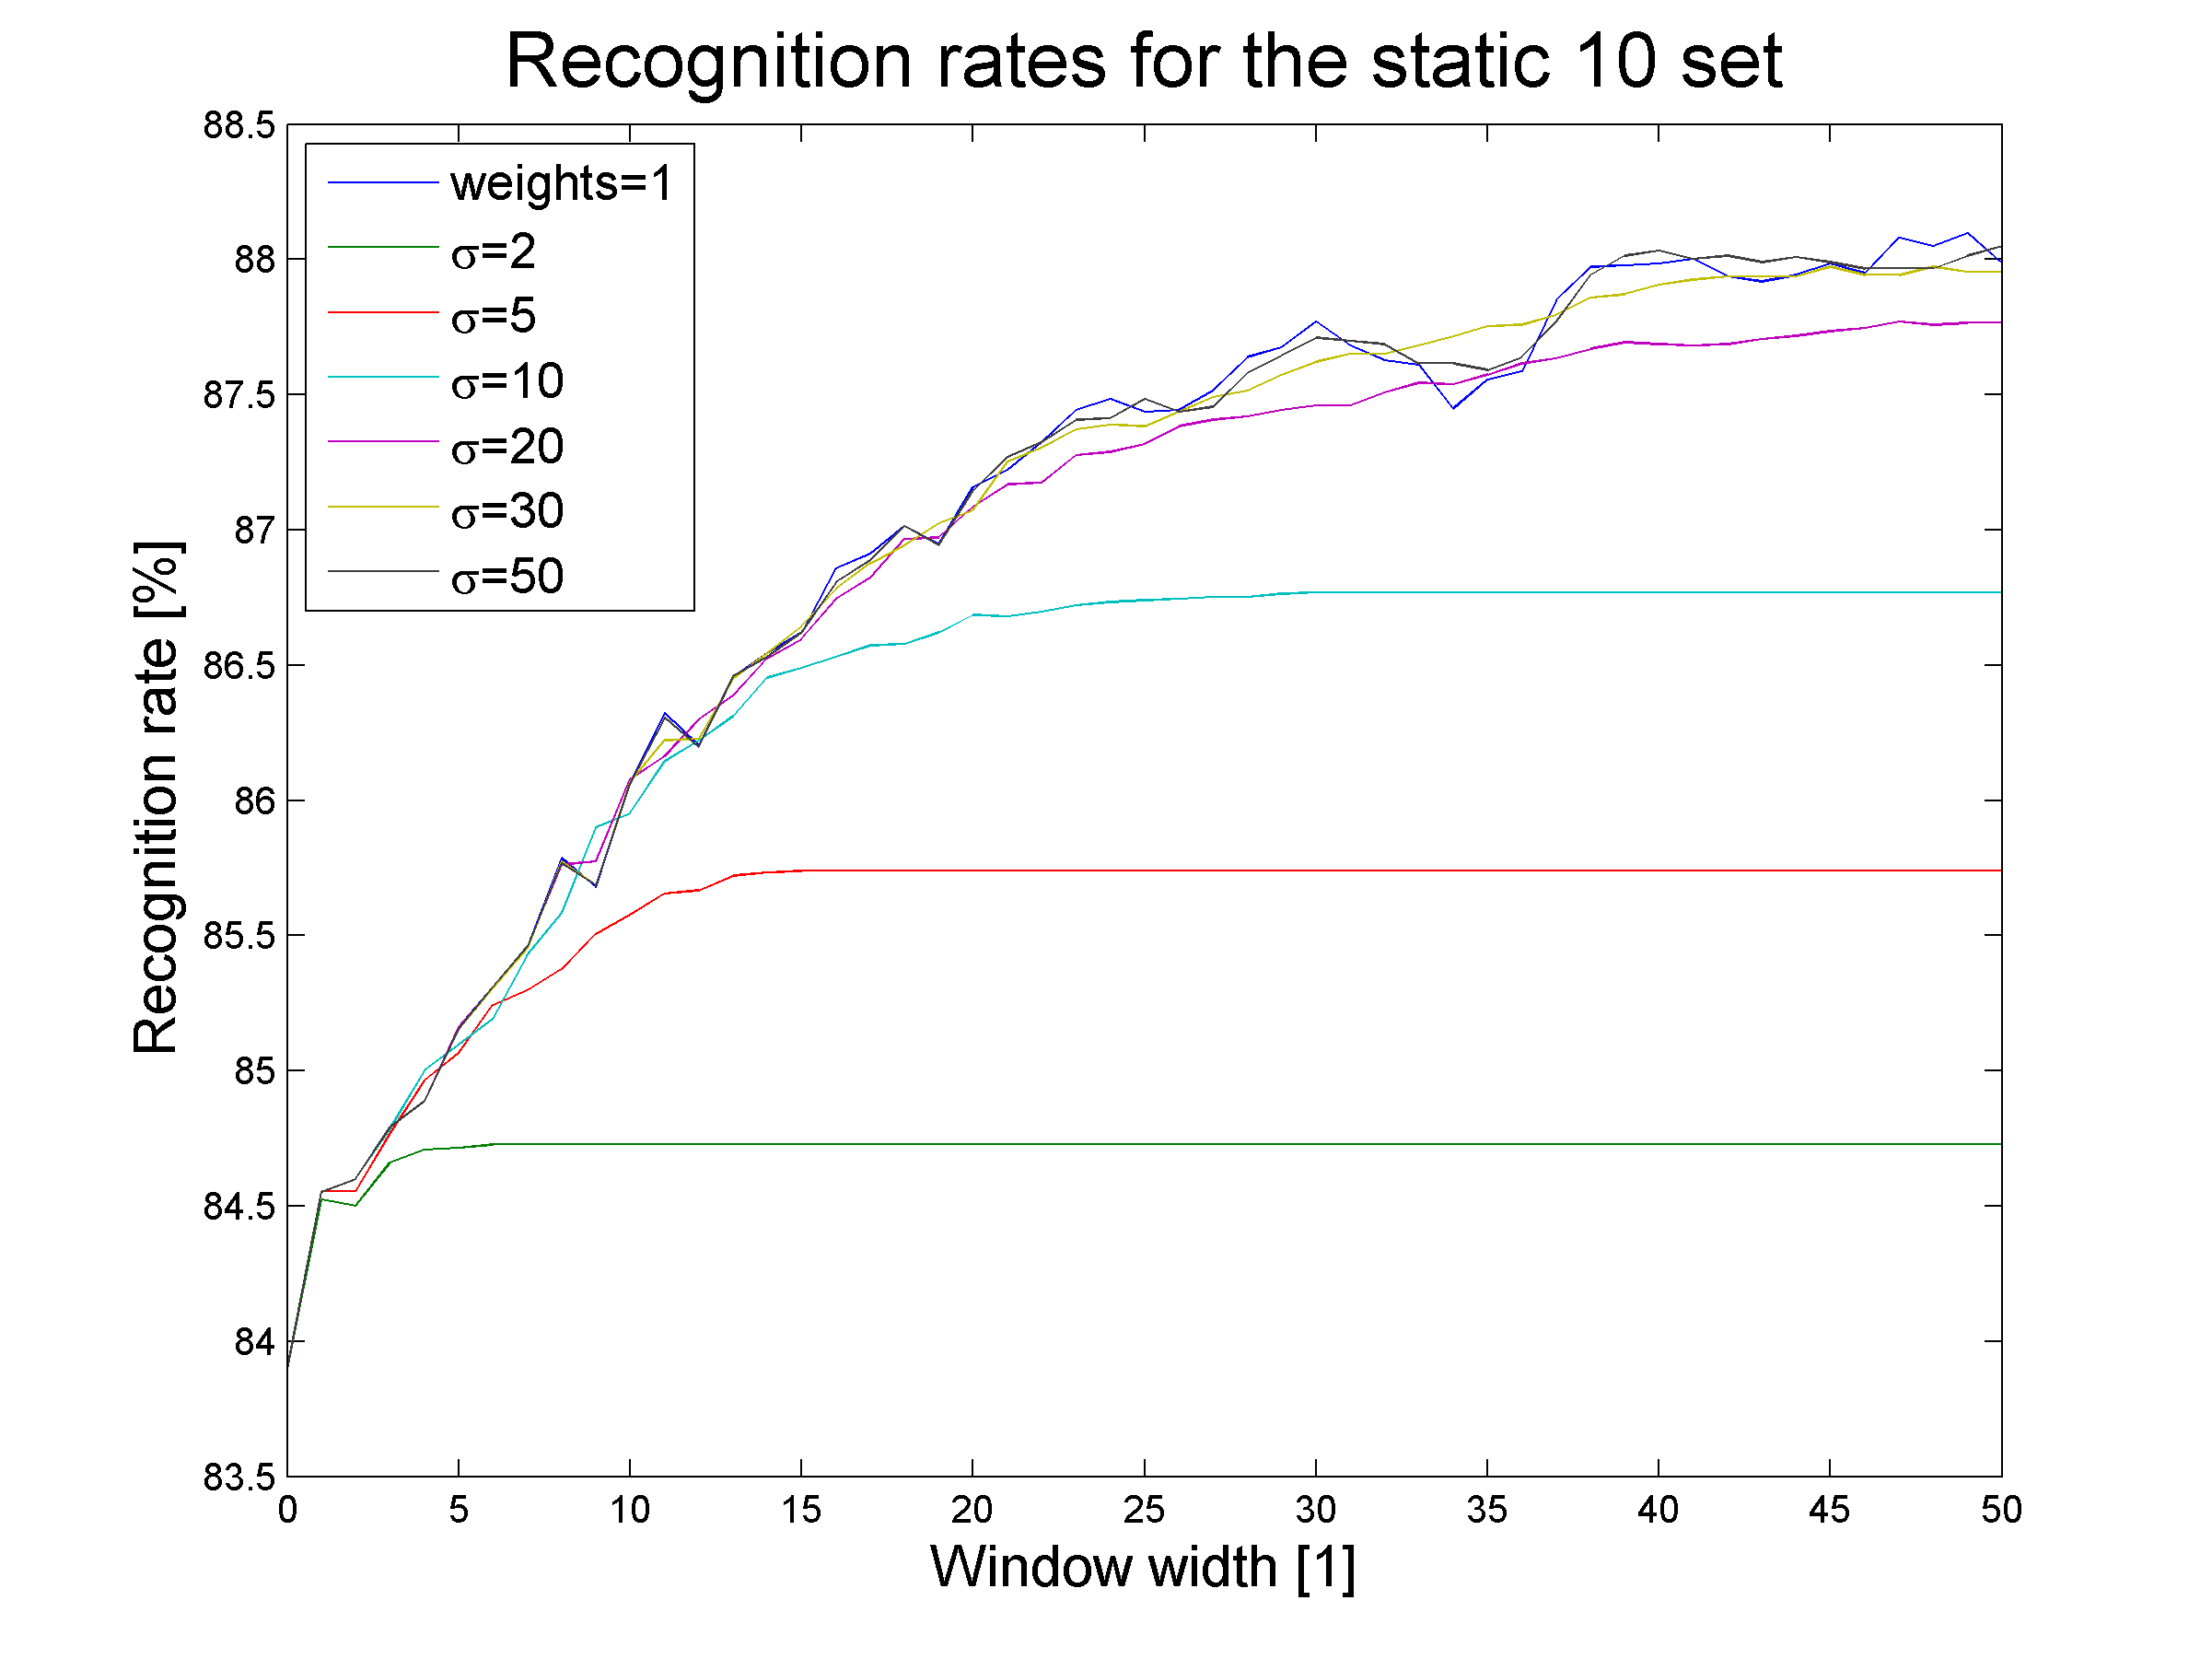
\includegraphics[width=0.5\textwidth]{figures/gaussSum10.png}
 }%
 \caption{Evaluation of weights for postprocessing distributed accordingly to normal distribution}
 \label{staticgauss}
\end{figure}

For this task, the half of the Gaussian distribution of weights can be used with maximal peak reached for the currently achieved result with weights slowly decreasing for measurements further away in time.
For Gaussian, the mean was assumed to be equal to $0$.
The standard deviation $\sigma$ was the parameter, which different values were tested.
The results were also performed for problems of recognition of 5 and 10 gestures.
The achieved results are presented in fig.~\ref{staticgauss}.
For 5 gestures, too small $\sigma$ prevented the increase of recognition rate due to the wider window size as the weights were equal to $0$. 
For greater sigmas, the achieved recognition rate is similar.
For this problem, the $\sigma$ equal to $10$ resulted in best recognition rate while the window was getting wider.
For problem of 10 static gesture recognition problem, greater sigma values achieved results comparable with the the results achieved with weights equal to 1.
As the usage of different weights also comes with greater computing cost and still did not result in better results, this part of processing can omitted without effecting the recognition.


From the presented results, the simple summation with uniform weights provides the greatest gain when it comes to the recognition rate and is the method recommended by the authors.


\section{Finger differentiation} 
Finger differentiation module is responsible to verify which particular fingers are detected during gesture recognition. The module can be used for additional processing on the user side, for which the information about the visible fingers can often be significant, It can also assist interpretation of data derived from parametrized gestures. The user can also use the module to better fit dataset features to the characteristics of selected gestures.
\subsection{Methods}
For this module were used the same classification algorithms (kernel functions) as those who had the best results in static gesture recognition. As in the case of static gesture recognition libSVM library has been used and RBF kernel has been selected.
\subsection{Evaluation methodology}
In the assumptions for static gesture recognitions was mentioned that the process must be independent of the position, rotation, sizes of hand and fingers. This presumption applies also to finger differentiation. However, this assumption is still does not contain one element, from which the differentiation process should be independent -- arrangement of hand. Whether forefinger is straight or bent, it is the same class, where only this one finger is taken out.

\subsubsection{Recorded dataset}
Dataset was collected by two different people. Each of them has recorded 32 classes, which reflect all the possible permutations of hand arrangements. The next step was to select from 32 gestures, those which are most frequently used by people in everyday life. Those 15 selected gestures are natural for human and do not cause a pain. People uses them as specific signes like peace sign. From the dataset were created four data collections used in the experiments:
\begin{itemize}
\item 32 gestures recorded by two people,
\item 15 gestures recorded by two people,
\item 32 gestures recorded by one person,
\item 15 gestures recorded by one person.
\end{itemize}

\subsection{Features}
As mentioned previously, it is important that the fingers differentiation process is independent of things like position of hand or size of finger. 

\begin{figure}[htb]
\centering
 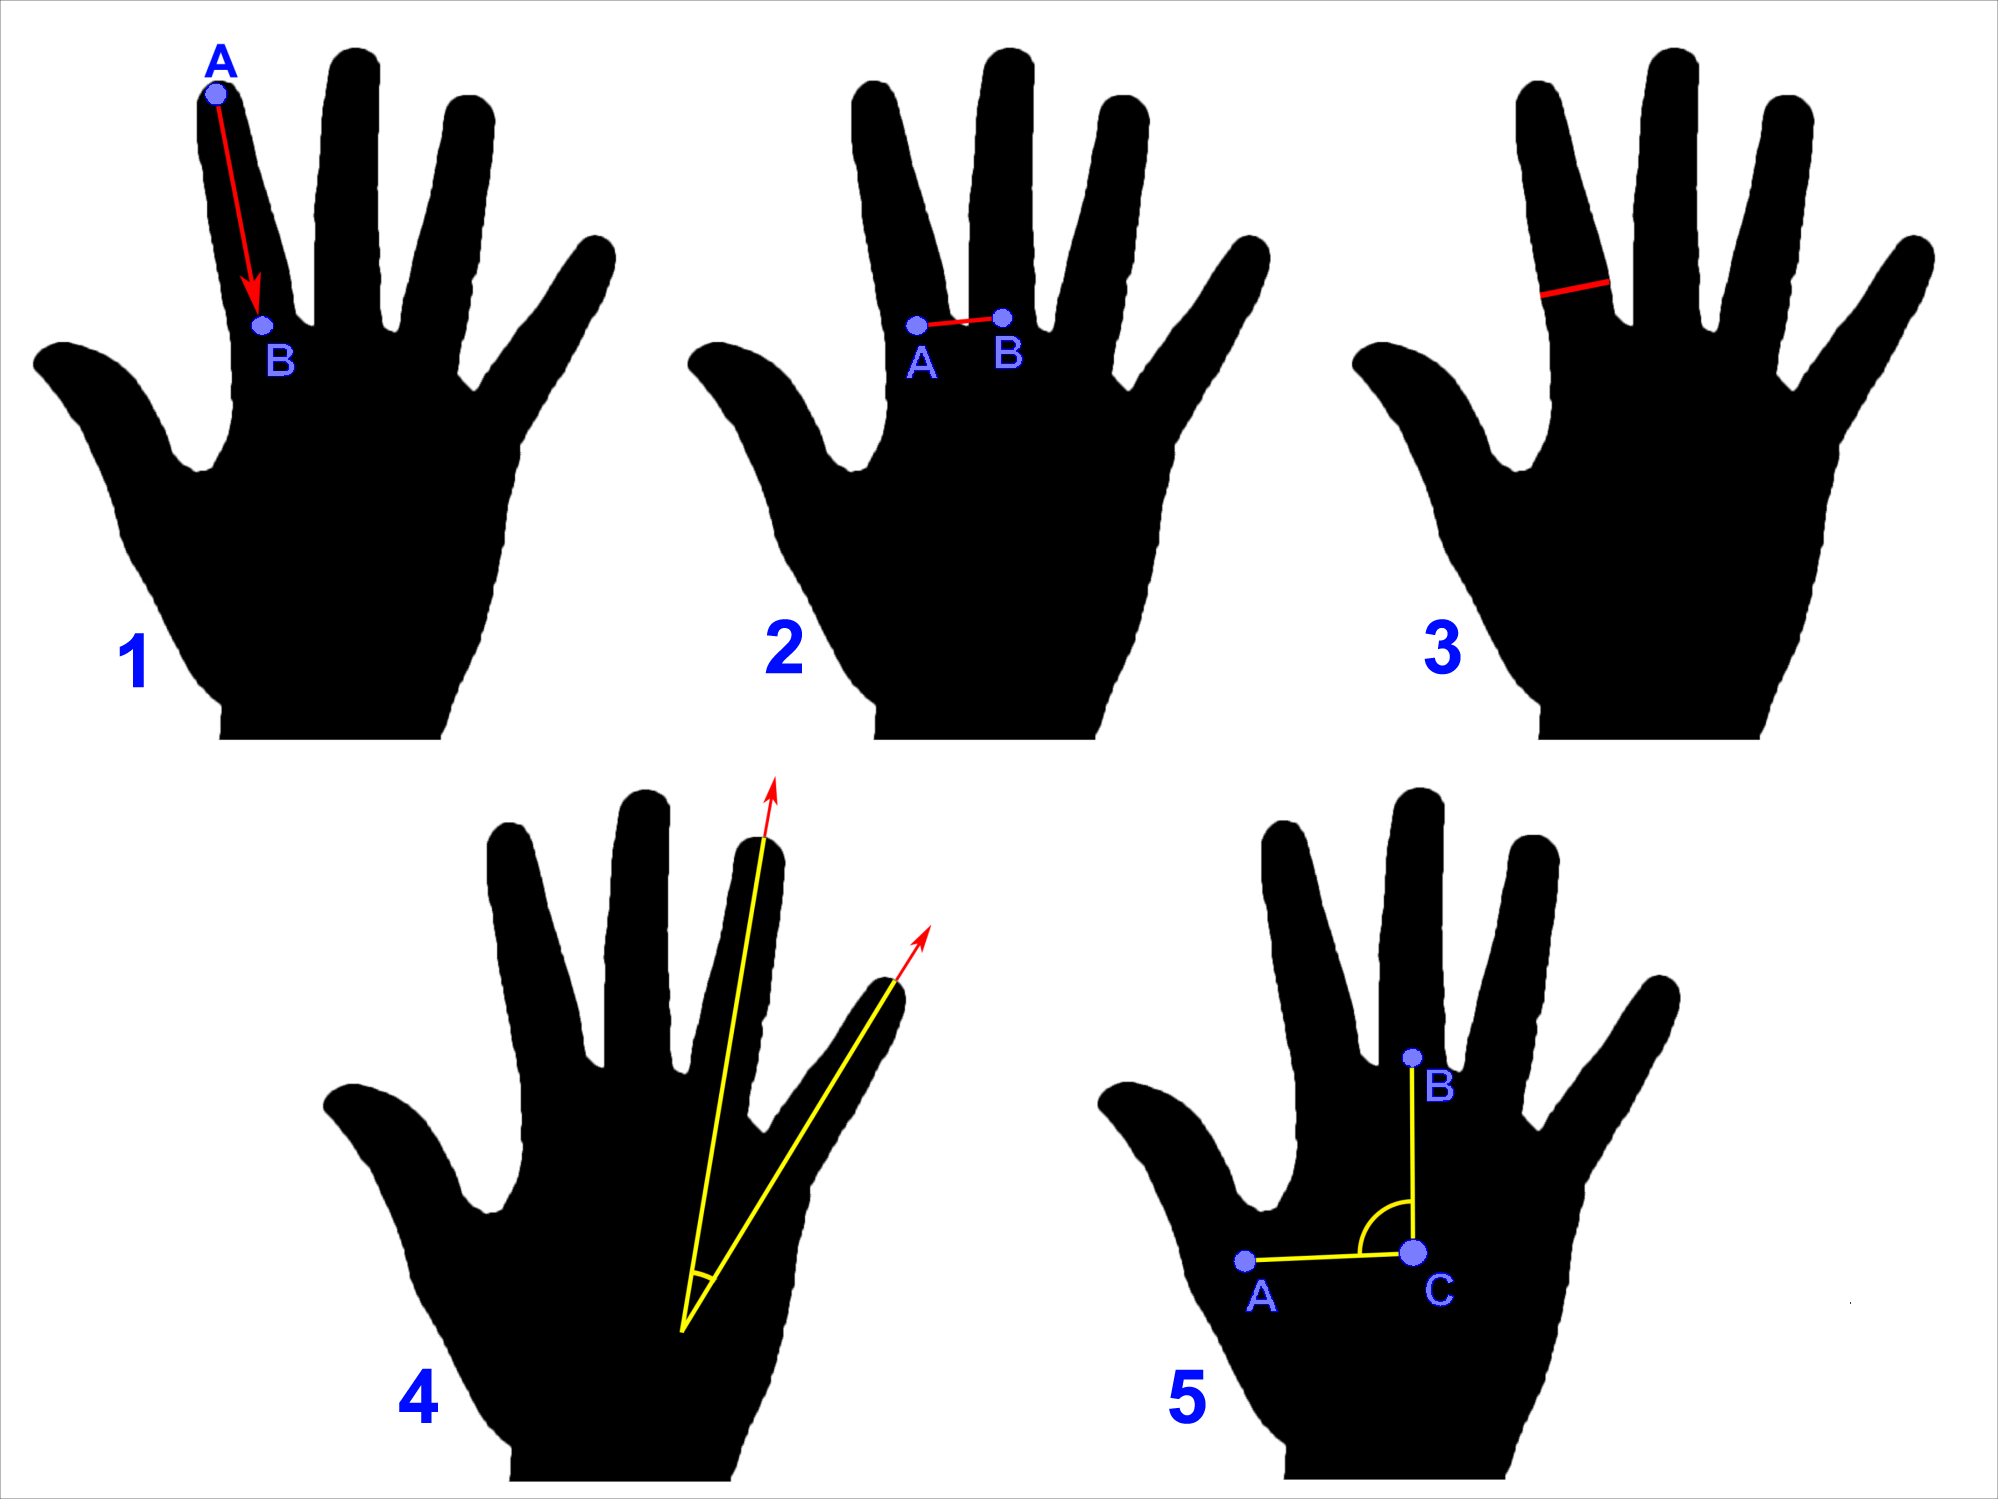
\includegraphics[width=0.75\columnwidth]{figures/fingDiffFeatures.png}
 \caption{Features used for finger differentiation}
 \label{fingfifffeatures}
\end{figure}

6 features were selected, which are independent of those parameters: 
\begin{enumerate}
\item finger count, 
\item distance between two nearest base points of a finger, 
To appoint a finger base point has to be reversed normalized direction vector multiplied by the length of a finger. Subsequent as the beginning of the vector thus formed is set finger tip position. The end of the vector indicates the finger base point (fig.~\ref{fingfifffeatures}.1). An example of distance between two nearest base points of a finger is showed on fig.~\ref{fingfifffeatures}.2.
\item ratio of the finger thickness to the maximal finger thickness, 
Leap Motion controller can return information about the thickness of the fingers (fig.~\ref{fingfifffeatures}.3). There are known relationships between the thicknesses of the fingers, for example that the thumb is the thickest finger. Just like in the previous feature ratio was used in order to become independent of size.
\item angles between two nearest fingers, 
In fig.~\ref{fingfifffeatures}.4  this feature has been shown. It is obtained by calculating the angle between the direction vectors of two adjacent fingers.
\item angles between finger and first finger relative to palm position. 
To calculate this angle three positions are needed : two finger tip positions and a palm position. The next step is to determine the line segments between palm position and finger tip positions. The searched angle is between two designated segments. This angle is marked in fig.~\ref{fingfifffeatures}.5.
\end{enumerate}

During testing new feature was created based on the features 2:\newline
2b. ratio of distance between two nearest base points of a finger to the minimal (non-zero) distance between two nearest base points
This feature is very similar to the previous one. The difference is that in this case is used ratio of distance and not the actual values. Thanks to this feature is independent of the size of hand.

\section{Experiments}
For the tests created several combinations of previously described features:
\begin{itemize}
\item 1,2,4
\item 1,3,5
\item 1,3,4,5
\item 1,2,3,4,5
\end{itemize}

All sets of features has been tested for all four datasets. The percentage results can be seen in table~\ref{findiff}. From the data obtained it can be concluded that the best match is when the all features are used. However, feature 2 is not independent of the size of the hand. Therefore, a new feature has been created using the ratio of two values obtained from the original feature. Then the test was performed for a set of: 1, 2b, 3, 4, 5 for all the dataset. The result for this test is in the last line of the table~\ref{findiff}. Interestingly, despite the fact that the modified feature is independent of the size of hand, attribute 2b had an inferior result than the original feature, which operates on the actual value of the distance apart fingers. 

\begin{table}[htp!]
\begin{center}
	\label{findiff}
	\caption{Results obtained by experimental feature sets for different data collections}
    \begin{tabular}{|c|c|c|c|c|}
    \hline
    features & 32 classes, 2 people & 15 classes, 2 people & 32 classes, 1 person  & 15 classes, 1 person  \\ \hline
    1,2,4		& 75.393\% & 87.288\%  & 78.411\% & 90.608\% \\ \hline
    1,3,5              	& 76.291\% & 87.504\%  & 79.638\% & 91.548\% \\ \hline
    1,3,4,5            	& 78.082\% & 87.504\%  & 79.638\% & 91.548\% \\ \hline
    1,2,3,4,5           & 83.180\% & 90.278\%  & 85.825\% & 93.036\% \\ \hline
    1,2b,3,4,5          & 76.553\% & 87.619\%  & 79.798\% & 91.629\% \\ \hline
    \end{tabular}
    \end{center}
\end{table}

It is worth to mention that it seemed that feature 4 -- angles between two nearest fingers -- will have a substantial contribution to finger differentiation. However, the results showed that this feature has impact only on the largest amount of data, while in other cases brought nothing.

In the second round of tests was verified how preprocessing will affect the finger differentiation process. For the best set of features from the previous test was performed a new test with preprocessing for all datasets. 

\begin{table}[htp!]
\begin{center}
	\label{findiffpre}
	\caption{The recognition rate achieved with feature set 1,2,3,4,5}
    \begin{tabular}{|c|c|c|c|c|}
    \hline
    features & 32 classes, 2 people & 15 classes, 2 people & 32 classes, 1 person  & 15 classes, 1 person  \\ \hline
    1,2,3,4,5           & \% & \%  & \% & \% \\ \hline
    \end{tabular}
    \end{center}
\end{table}



\chapter{Detection of dynamic gestures}

\section{Proposed methods}

The dynamic gesture recognition problem is a problem, where the input data consist of a list of consecutive positions and orientations of hand and fingers. 
Moreover, the important factor for recognition is the time dependencies between sequences of hand and finger positions.
Another challenge comes with the fact, that the gestures performed slower and faster should be recognized as the same dynamic gesture.

The proposed solution utilizes parts of the solution used for recognition of the static gestures.
Each frame of the captured data is described by the feature set similarly to the static solution presented in Chapter~\ref{staticChapter}.
The set of features for each frame is then processed by the Hidden Markov Model scheme. 

\subsection{Hidden Markov Model}

A HMM can be considered a finite, $N$-element set of states (a graph), which are associated with the probability distribution.
A Hidden Markov Model is model of a system with the Markov property.
The Markov property means that the next, future state depends only on the previous state and probability of transition between those states.
The first introduction of HMM comes from the work of L. E. Baum et al. \cite{hmmfirst}, who proposed the mathematical background for HMMs.

The transitions between states are represented by the transition probabilities usually stored in $N \times N$ matrix $T$.
In every state, one of the observation from the finite, $K$-element observation set can be generated with observation probability usually represented by the $N \times K$ emission matrix $E$.
The finite set of all possible observation is called the alphabet.
The HMM also consist of a $N$-element vector of initial state probabilities $\Pi$ of the hidden starting state.
Each HMM can be fully defined by the ($T$, $E$, $\Pi$).

\begin{figure}[htbp!]
\centering
 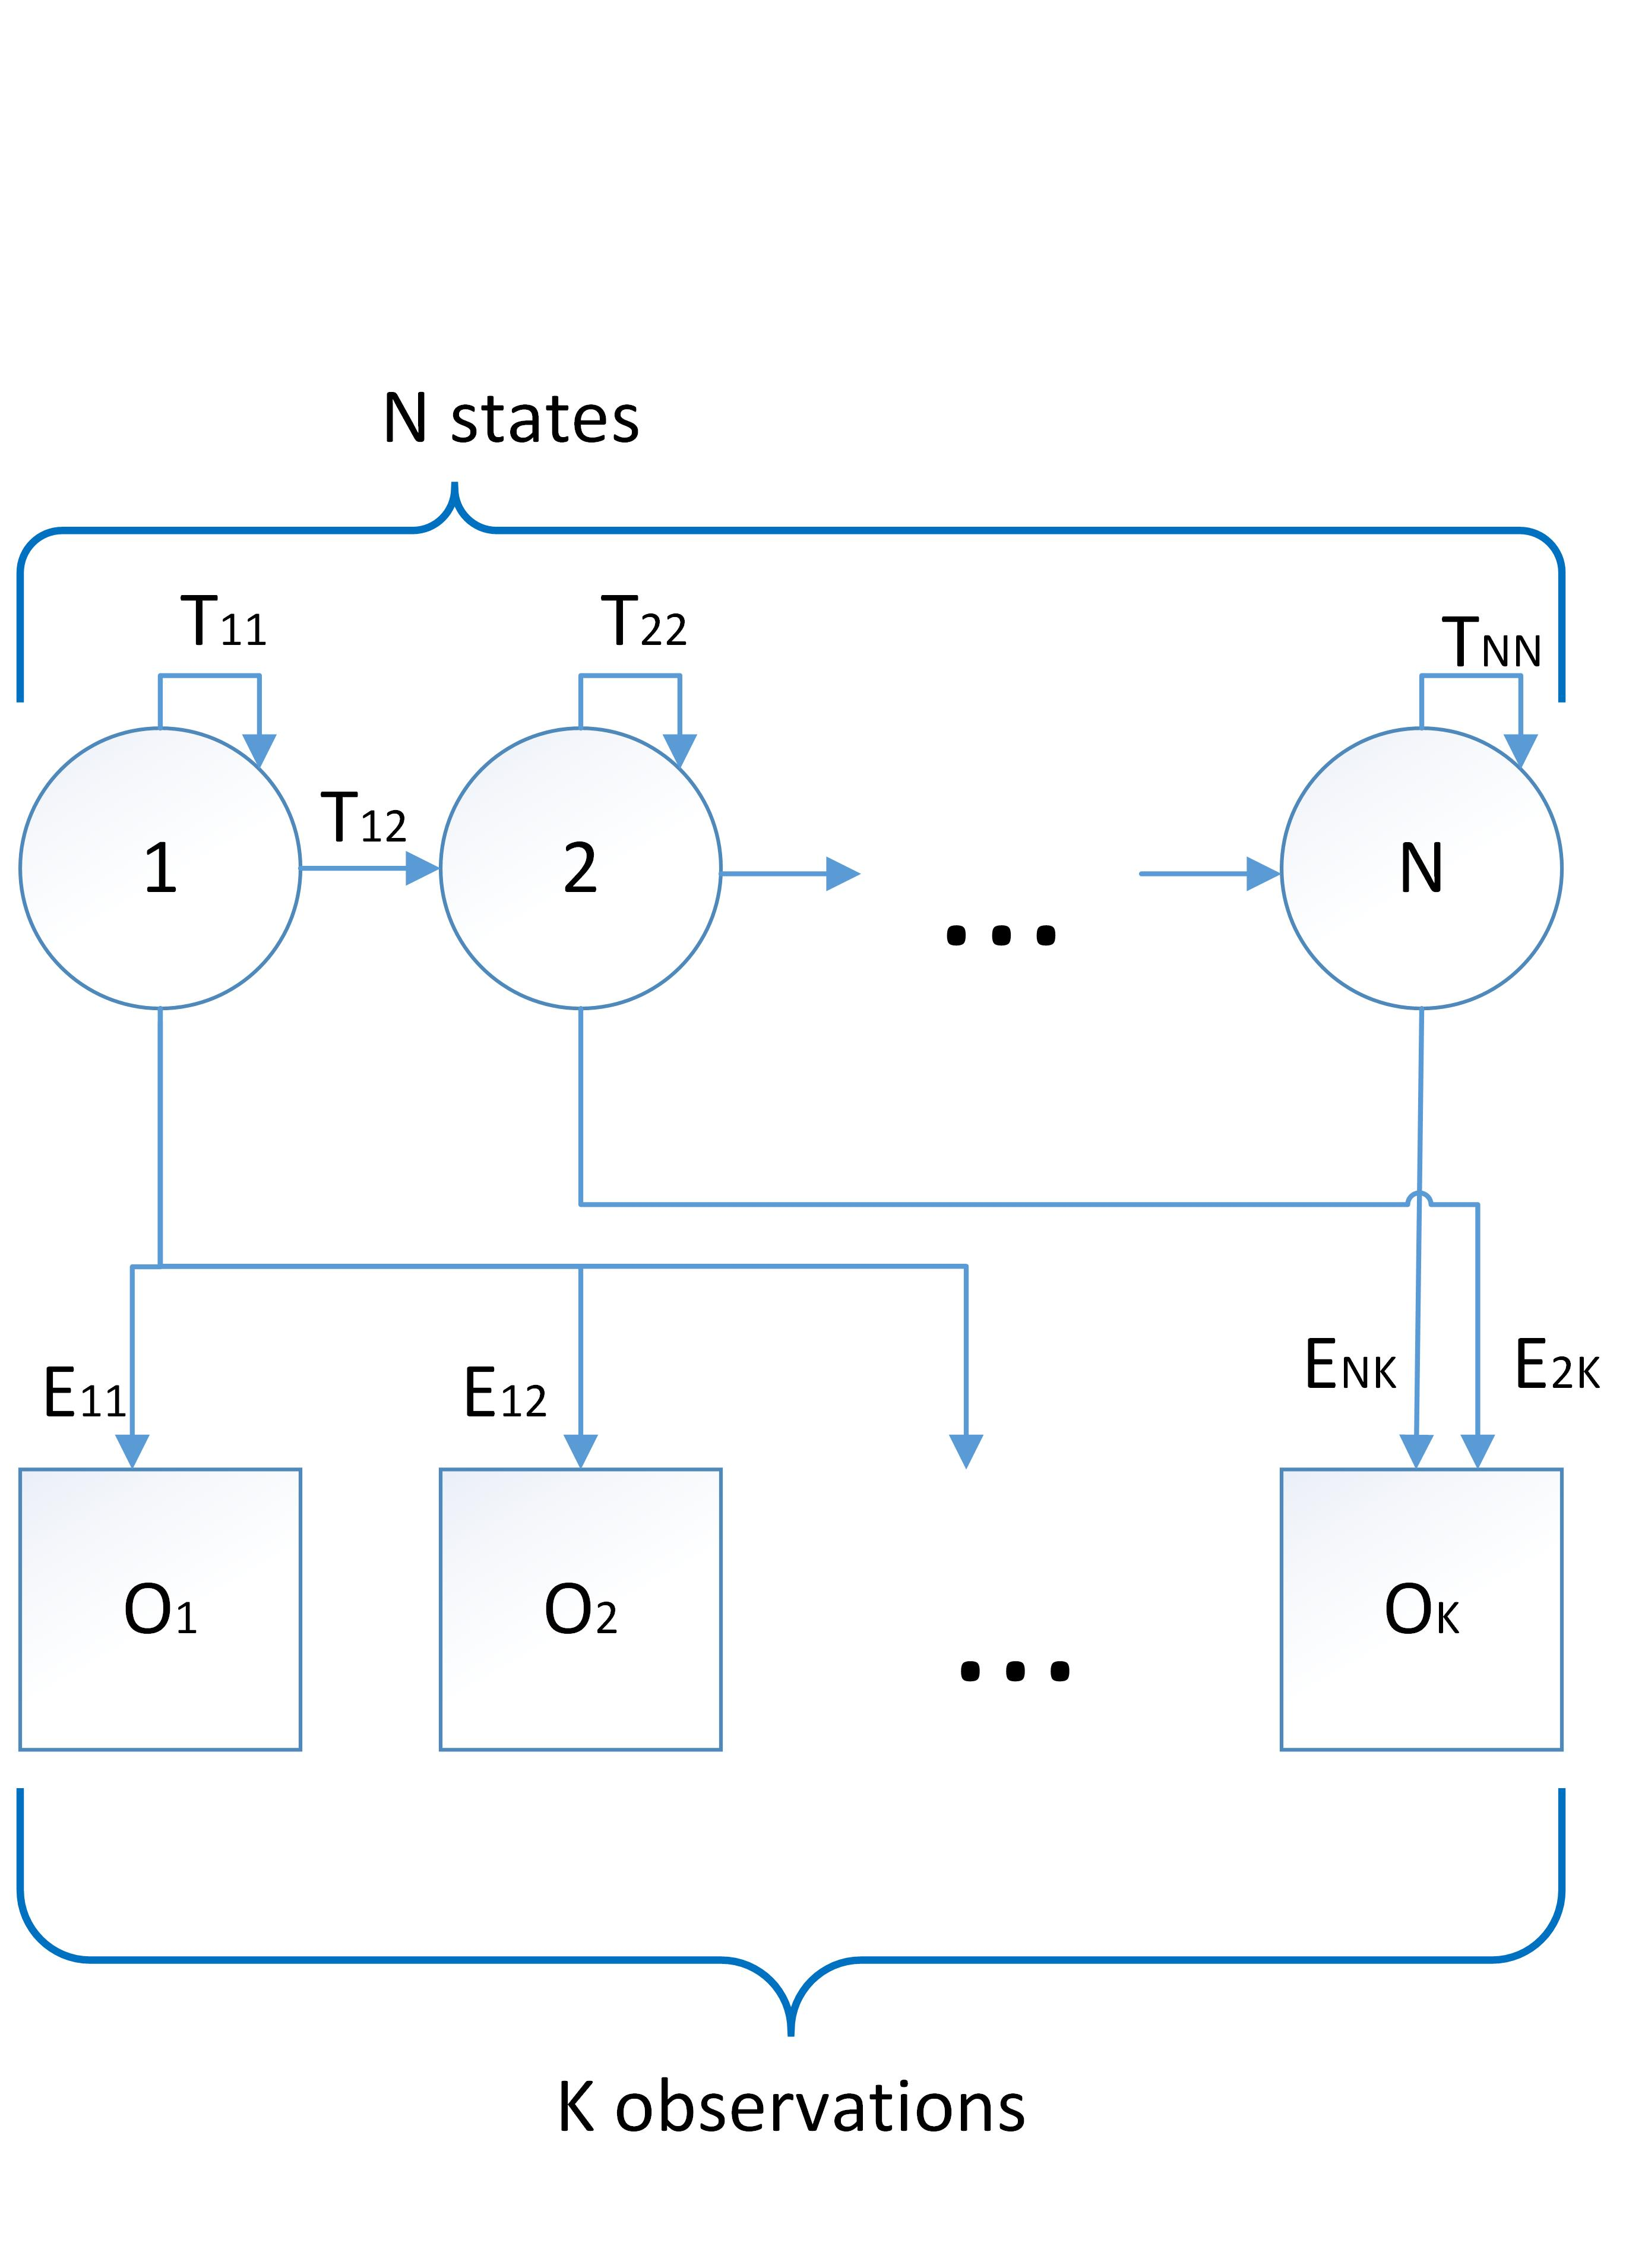
\includegraphics[width=0.7\columnwidth]{figures/HMM1.jpg}
 \caption[]{A simple Hidden Markov Model (HMM) consisting of N states and K possible observations}
 \label{dynamicgestureswiki}
\end{figure}


The example HMM can be seen in Fig.~\ref{dynamicgestureswiki}.
The HMM in the figure consists of $N$ states $\{1, 2, 3, ..., N\}$ and $K$ possible observations $\{O_1, O_2, ..., O_k\}$.
The probabilities $T_{ij}$ define the transition probability from state $i$-th to state $j$-th. 
The probabilities $E_{ij}$ define the observation probability of generating $j$ observation while being in state $i$.
The non-zero transition and emission probabilities are represented in Fig~\ref{dynamicgestureswiki} by arrows.

The HMM can be understood as a directed graph with two types of weighted vertices. 
This way, each state is represented by one type of vertices while observations can be shown as second type of vertices.
There are no edges between vertices representing observations.
The probability values for edges are stored in $T$ and $E$ matrices.

There are three main algorithms used with the HMMs:
\begin{itemize}
\item Forward-Backward algorithm \cite{hmmtutorial, hmm}, 
\item Viterbi algorithm \cite{hmmtutorial, hmm},
\item Baum-Welch algorithm \cite{hmmtutorial, hmm}.
\end{itemize}

The algorithms are shortly described in the following subsections.

\subsection{Forward-Backward Algorithm} 

The Forward-Backward algorithm is used to find the posterior probability of given states given the set of observations.
Given the set of $N$ hidden state variables $X = \{X_1, X_2, ..., X_N\}$ and a sequence of $t$ observations $o_{1:t} = \{o_1, o_2,...,o_t\}$, the algorithm computes probability of state given the observed sequence $P(X_i | o_{1:t})$.
The algorithm utilizes a dynamic programming approach, by performing three steps in a loop: 
\begin{enumerate}
\item computing forward probabilities,
\item computing backward probabilities,
\item computing smoothed values.
\end{enumerate}
The forward pass phase for all states $i=1,..,N$ computes probability $P(X_i | o_{1:k})$, where $k$ is smaller than t, which represent the probability of ending up in state $X_i$ after first k observations. 
The backward pass computes probability $(P(o_{k+1:t}) | X_i)$, which are the probabilities of observing the rest of the observations from the state $X_i$.
The smoothing part uses Bayes rule to compute the probability of state $X_i$ given the whole observation sequence:
\begin{equation}
P(X_k | o_{1:t}) = P(X_k | o_{1:k}, o_{k+1:t}) \propto P(o_{k+1:t} | X_k) P(X_k | o_{1:k}).
\end{equation}
The time complexity of this algorithm is $O(N^2 T)$, where $T$ is the length of observation sequence and $N$ is the number of possible states.


\subsection{Viterbi Algorithm}

The Viterbi algorithm is used to find the most likely sequence of hidden states that best explain the set of observations.
The set of those states is called the Viterbi path. 
The path can be found using the dynamic programming and implementing the equations:
\begin{equation}
\begin{cases} V_{1,k} = P(o_1 | k)  \Pi_k & \mbox{for } k = 1..N \\ V_{t,k} = P(o_t | k)  \argmax_{x\in X} (a_{x,k}  V_{t-1,x}) & \mbox{for } k = 1..N\mbox{ and } t = 2..T \end{cases}
\end{equation}
The solution can be understood as finding a path with maximum probability $\argmax_{x\in X} (V_{T,x})$. 
The time complexity of the algorithm is $O(N^2 T)$, where N is the number of states and T is the observation length and is equal to the complexity of the Forward-Backward algorithm.

\subsection{Baum-Welch Algorithm}

The Baum-Welch algorithm is the algorithm used to find the unknown parameters of the HMM.
For each training example, the algorithms computes the state transition probabilities, observation probabilities in each state and initial probabilities, which maximize the likelihood of observed sequence.
Having the set of sequences of observations, the algorithm can be used to train HMM to detect the sequences similar to the ones used in learning process.
The algorithm uses the results obtained by the Forward-Backward algorithm to iteratively update the probabilities in the emission and the transition matrices.
The training process is stopped after the desired level of a convergence is reached.


\subsection{Structure of the HMM}

\begin{figure}[htbp!]
\centering
 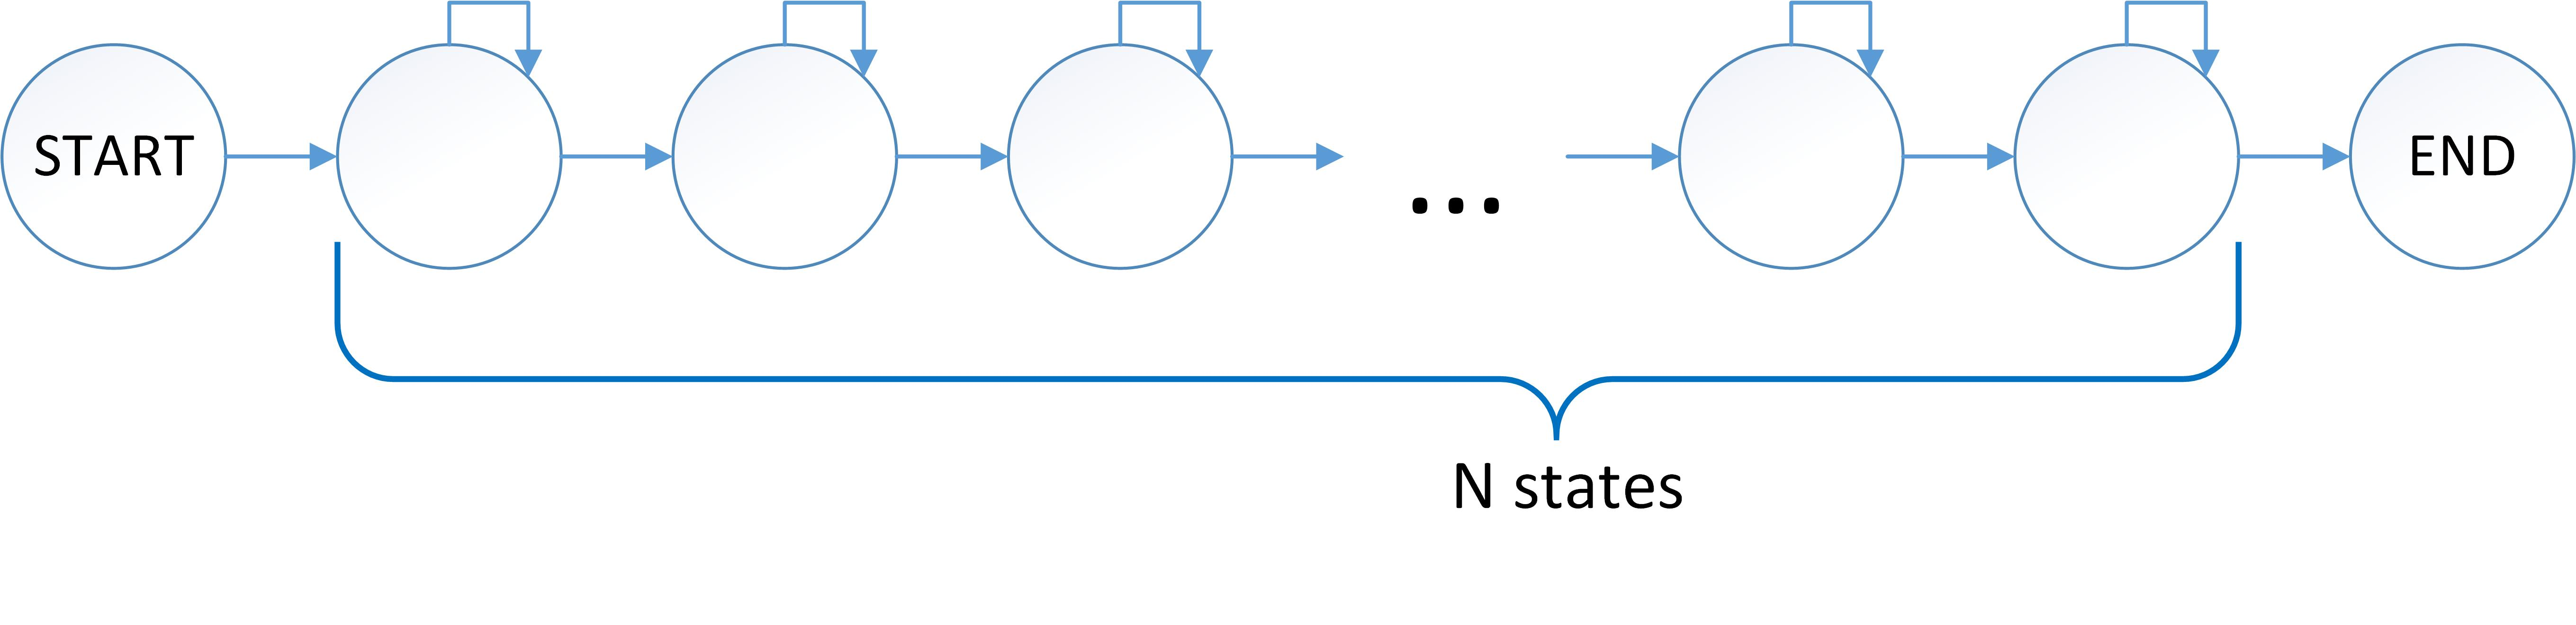
\includegraphics[width=1\columnwidth]{figures/HMMSingle.jpg}
 \caption{Structure of the HMM's states and non-zero transitions used to detect a single dynamic gesture}
 \label{singlehmm}
\end{figure}

In the dynamic gesture recognition task, we adopted a structure of HMM where each state has non-zero transition probabilities to itself and to the next state in the sequence.
The proposed structure is presented in Fig.~\ref{singlehmm} and was proposed by Yang et al.~\cite{hmm}.
The states can be understood as the phases of hand movement that happen when a wanted gesture is performed.
The self-transitions are used to model the different speeds of the gestures and thus allow to achieve a more robust system.
This structure after training process can be used to measure the probability that the dynamic gesture occurred given the set of observations.



Having the single dynamic gesture recognition problem modelled as the sequence of $N$ states in which $k$-th state is connected by the edges to the $k$ and $(k+1)$ state and to the all observations.
The problem of distinguishing $M$ gestures translates to the problem of computing probabilities for $M$ sequential graphs.
The problem of finding whether and what dynamic gesture occurred is the problem of finding the probabilities from each of the $M$ HMMs.
Alternatively, the $M$ HMMs can be combined into one HMM were those single HMMs are treated as parallel paths.
The structure of proposed single HMM is presented in Fig.~\ref{HMMstructure}.
In this structure, the recognition process is a process of finding, which of the parallel paths is the most probable.

\begin{figure}[htbp!]
\centering
 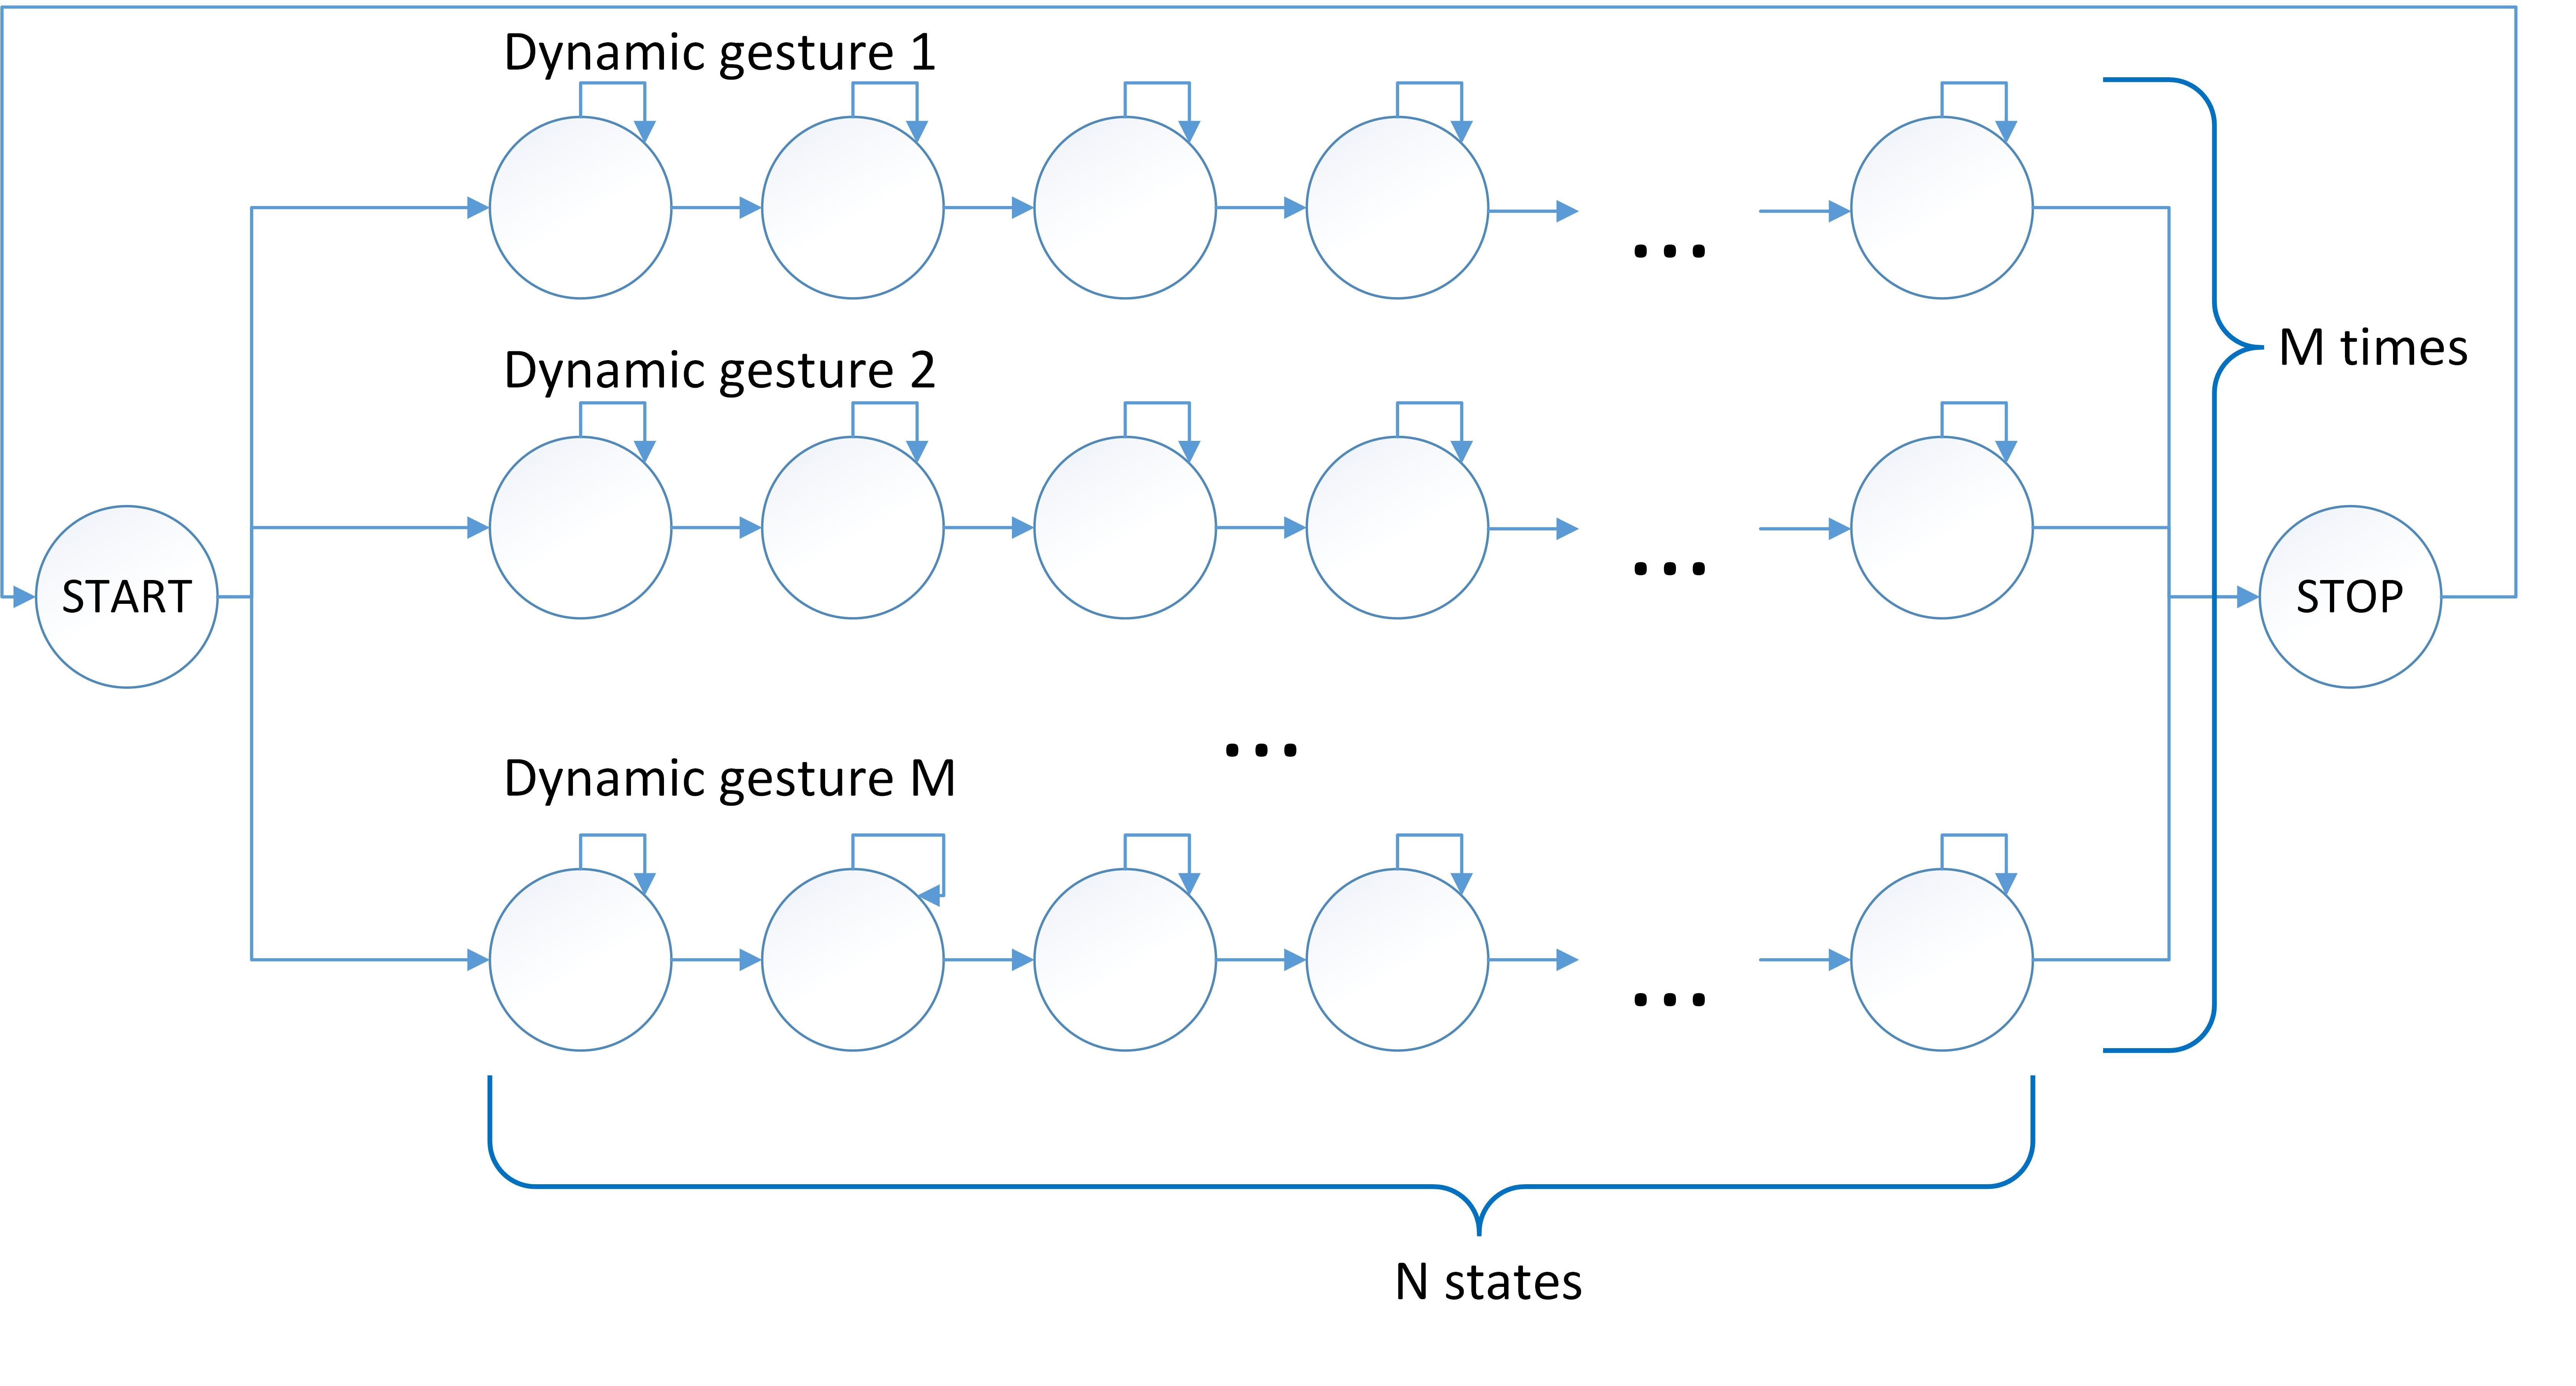
\includegraphics[width=1\columnwidth]{figures/HMM_eng.jpg}
 \caption{Structure of the HMM's states and non-zero transitions used to simultaneously detect one of $M$ dynamic gestures}
 \label{HMMstructure}
\end{figure}

\subsection{HMM observation from Leap Motion data}

One of the problems when designing the system is a problem of correctly preparing the set of observations from the Leap Motion data.
Most of the proposed solutions in the literature assume that the observations are one-dimensional~\cite{hmmtutorial, hmm}.
This poses a challenge as the raw data from Leap Motion is high-dimensional.
This is the reason, why it is needed to reduce the dimensionality of the observation of the single hand in the predefined moment in time.

To do this, unsupervised clustering algorithms were introduced. 
For this task we examined 3 methods:
\begin{itemize}
\item Chinese whispers \cite{CW1, CW2},
\item Girvan-Newman clustering \cite{Newman},
\item k-means with additional methods to determine the number of clusters. \cite{kmeans1, kmeans2}.
\end{itemize}

\subsubsection{Chinese whipsers}
Chinese whispers algorithm is an efficient randomized graph-clustering algorithm, which is time-linear in the number of edges.
The algorithm was proposed in work by Biemann~\cite{CW1} and thoroughly examined in Natural Language Processing problems. 
The main advantage of the algorithm is the ability to independently determine the number of classes. 
In tests, we used the implementation available in dLib-ml library~\cite{dlib}, which provides multiple implementations of machine learning algorithms.

\subsubsection{Girvan-Newman clustering}
Girvan-Newman clustering is a hierarchical algorithm used to detect clusters in a data represented as a graph.
The algorithm progressively removes edges from the original network until it reaches the maximal number of iterations or an error condition is met.
An adjacency matrix is used to represent the edges between data, where edge value is the similarity between two data points.
The algorithm iteratively calculates the eigenvalues of a created matrix using the power iteration method. 
In case of a complete graph, this algorithm is relatively slow.

\subsubsection{K-means clustering}
Another proposed approach is k-means clustering algorithm.
The idea for the algorithm comes from polish mathematician Hugo Steinhaus, but the first practical application has been presented by MacQueen~\cite{kmeans2}.
The algorithm initially randomly selects $k$ starting points and iteratively performs two steps utilizing the idea of expected-maximization~\cite{expectedmaximization}:
\begin{enumerate}
\item For each data sample the algorithm calculates the distances to $k$ centroids and labels the samples with the label of the centroid with the smallest distance.
\item For each class, the algorithm recalculates centroids position to the averaged position of all samples belonging to class.
\end{enumerate} 
The algorithm stops after the maximum number of iterations or when the change between two consecutive iterations is smaller then defined value.
Unfortunately, the algorithm requires prior knowledge of the number of expected classes.
Nevertheless, there exist heuristics methods aiding in correctly choosing the number of classes. 
One of those methods is plotting the sum of squares error(SSE) between elements within each class against the number of chosen classes. 
The plot is then visually inspected and the fall in error is sough.
The argument for which the drastic error drop is observed is believed to be the correct number of classes in the provided data.

Another, more formal approach introduces the measure of dissimilarity and is called Silhouette width \cite{silhouette}.
Declaring $a(i)$ as the average dissimilarity measure to other samples in the same cluster and $b(i)$ as the lowest average dissimilarity measure to samples in the other clusters which $i$ is not a part of.
The measure of each cluster corrected is proposed to be computed by:
\begin{equation}
s(i) = \frac{b(i) - a(i)}{\max{\{a(i),b(i)}\}}
\end{equation}
The big value of $s(i)$ implies good clustering, while small value of $s(i)$ suggests that the number of classes was not properly chosen.
The $s(i)$ values are used to find the proper number of clusters.


\begin{figure}[htb]
\centering
 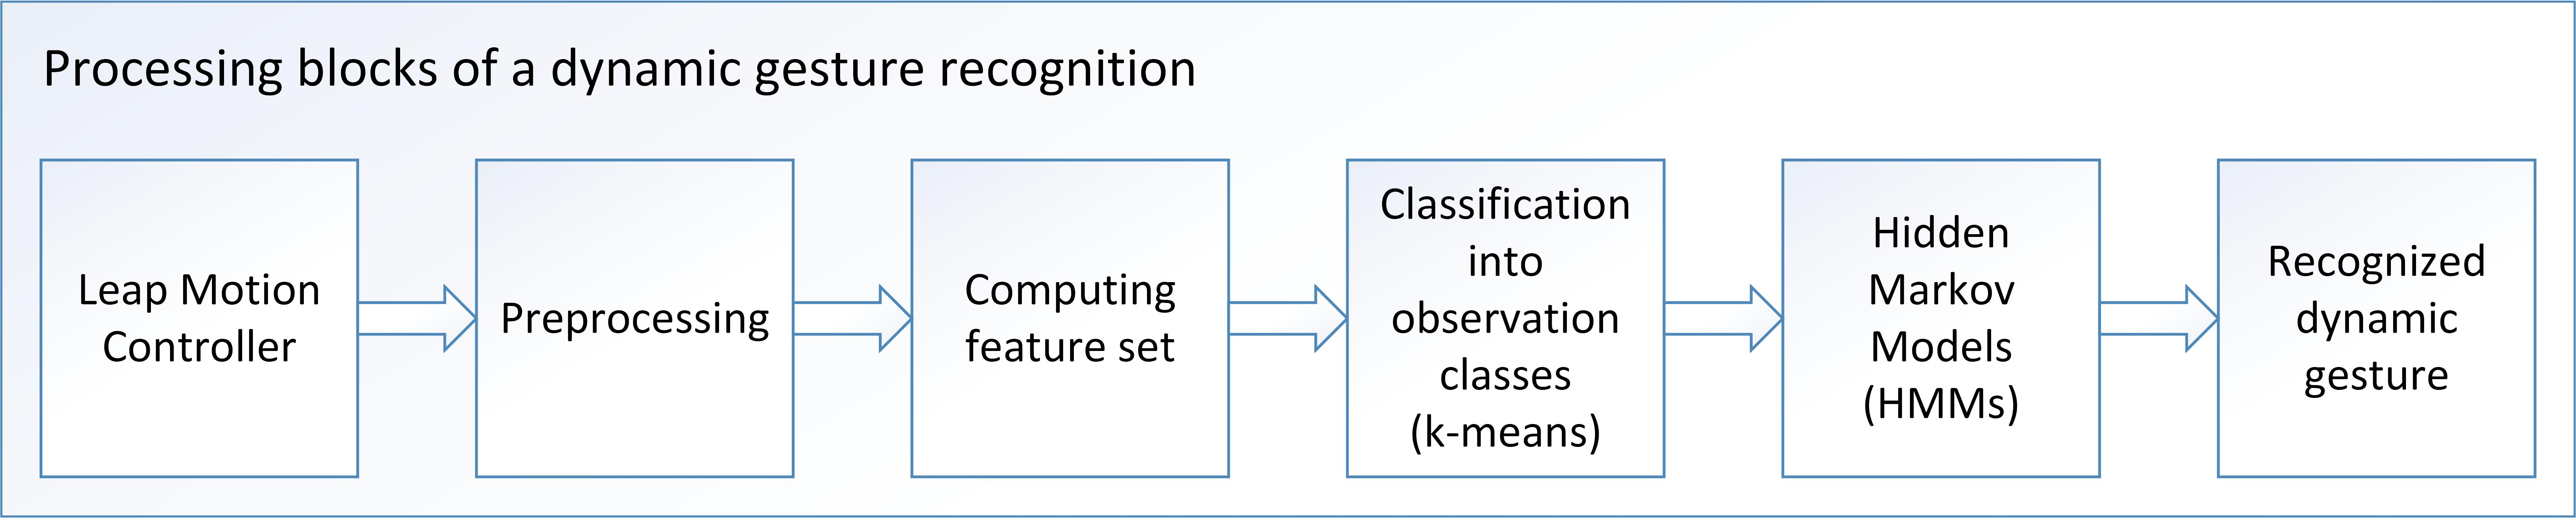
\includegraphics[width=1\columnwidth]{figures/DynamicGestures2.jpg}
 \caption{Solution blocks of learning and testing parts used in the dynamic gesture recognition}
 \label{dynamicgesturesflow}
\end{figure}

\subsection{Whole processing algorithm}
The designed processing algorithm is presented in Fig.~\ref{dynamicgesturesflow}.
The solution consists of two parts: an offline learning and an online recognition.
In learning part, the raw data is preprocessed and then the feature set is extracted. 
Those features are extracted for all recorded positions in training data.
Then one of the unsupervised clustering algorithms is used to find the clusters in the data and then classify those feature sets into observation clusters.
Computed sequences of observation classes represent each dynamic gesture as a series of one-dimensional observations.
For each dynamic gesture, the corresponding HMM is learnt using the Baum-Welch algorithm on the sequence of observations.
The Baum-Welch algorithm computes the matrices that maximizes the probability for one sequence of observations. The problem of training on multiple training data was encountered.
Using the idea presented by Petrushin~\cite{hmmtutorial}, where each matrix trained by one training example is incorporated into hmm's transition matrix using addition with a learning rate $\mu$.
Denoting the transition matrix of HMM by $T$ and learnt transition matrix $T_{new}$, it can be written:
\begin{equation}\label{eq:dynT}
T = (1-\mu) \times T + \mu \times T_{new}.
\end{equation}
The same idea is applied to the emission matrix $E$ and learnt emission matrix $E_{new}$:
\begin{equation}\label{eq:dynE}
E = (1-\mu) \times E + \mu \times E_{new}.
\end{equation}
The learning rate $\mu$ is a value between 0 and 1.
Smaller learning rates results in slower learning, but bigger values may result in no convergence of learning. 
Finding correct learning rate is a task of one of the experiments.
Another problem encountered using this approach is the fact, that matrices no longer represent the probability as the total values in rows do not add to $1.0$.
Therefore, each row of new matrices is normalized to $1.0$.

When dealing with multiple training examples, the learnt solution may adapt to the training samples, but perform poorly on the testing set. 
The problem is known as overfitting to the training samples.
To deal with potential problem, the k-fold cross validation was utilized in a similar approach as in the static gestures presented in Chapter~\ref{staticChapter}.
To complete the training process, each trained HMMs is combined into one recognition structure.

In the recognition, the raw data from Leap Motion is preprocessed, then each frame is labelled accordingly to the classes learnt by the unsupervised clustering algorithm.
The next step includes providing the set of observations to HMMs and running the Viterbi algorithm.
The Viterbi algorithm computes a probability of the the most likely sequence.
Then the maximum probability for each HMM is calculated.
If the maximum probability is above threshold, the gesture is assumed to be correctly recognized with the label of the HMM with the maximum probability sequence.


\section{Evaluation methodology}\label{dynamic:set}

To evaluate the quality of recognition achieved by proposed processing pipeline, $6$ dynamic gestures were chosen.
For each of those gestures, we recorded 120 samples (30 samples per each author).
The recorded data contains recordings in different positions with respect to the Leap Motion coordinate system and with different speeds to measure the wanted invariance and robustness of the proposed approach.
The chosen dynamic gestures are:
\begin{enumerate}
\item ``123'' -- counting to three using fingers of one hand,
\item ``door'' -- it's a gesture performed while trying to grasp a handle of a door and then open the door,
\item ``circle'' -- making a circle in the air with the forefinger,
\item ``scissors'' -- simulating cutting an object with scissors made by a forefinger and a middle finger,
\item ``gun'' -- a thumb and an index finger are up with rest of the fingers in a fist. The hand moves up simulating a firing from a gun.
\item ``moving the object'' -- performing the task of grasping an invisible object, moving it and letting it go in a different place.
\end{enumerate}

The $120\times6=720$ samples were divided into training set containing $66,7\%$ of recordings and testing group containing the remaining $240$ recordings. 
The recorded dataset was called the dynamic 6 set.
The part of the gestures recorded by Katarzyna were used to find the proper number of observation clusters
The training set was used to train each HMM separately on the training data of each gesture.
Preliminary results revealed that initialization of HMM matrices has an impact on the achieved results.
Due to no prior knowledge, the random initialization was chosen.
This approach did not yield reliable solutions in all situation and therefore each training process is performed $10$ times and a model with the best recognition rate from cross-validation is returned.  
Each training cycle of all HMMs takes $1-10$ minutes, with total training part taking $25-60$ minutes.
If not stated otherwise, the learning rate $\mu$ was set to $0.1$, k-cross validation was performed for $k=5$ and the number of states in one HMM was set to $10$.


\section{Experiments}
The experiments are divided into subsections, where in one subsection impact of one parameter is tested.
In first subsection, the number of observation clusters using only the dataset is examined.
The second subsection contains experiments involving different feature sets.
Those subsections are followed by tests involving the impact of number of observation clusters on the total recognition rate of dynamic gestures.
In subsection four, different learning rates are examined. The last subsection presents the impact of the state count on the recognition rate. 

\subsection{Number of observation clusters} \label{numberOfClasses1}

The performed experiments started with testing the unsupervised clustering methods to determine the correct number of observations.
Based on the successful static gesture recognition, each of the hand poses was represented by the vector of values containing:
\begin{itemize}
\item a number of detected fingers,
\item the $5$ greatest angles between the finger's tip vector and palm normal,
\item the $5$ greatest angles between the finger's tip vectors,
\item the $5$ greatest distances between the tip positions of fingers.
\end{itemize}
In order to measure a difference between hand poses, the distance function was introduced as the L2 norm between feature vectors for each hand pose:
\begin{equation}
d(x,y) = \sqrt{ \sum_{i=1}^{16} (x_i - y_i)^2 }
\end{equation}
The Chinese whispers and Girven-Newman algorithms use the similarity function $s(x,y)$ which was defined using the difference function $d(x,y)$: 
\begin{equation}
s(x,y) = \frac{1.0}{ \max{\{d(x,y), eps\}}}
\end{equation}
where $eps$ was the numerical epsilon.

For the Chinese Whispers and Girven-Newman clustering the typical parameters from dlib-ml library were used --- the Chinese Whispers maximal iterations were set to $100$, while the Girven-Newman algorithm was run with maximal iterations equal to $2000$ and precision epsilon was equal to $1e-4$.
For the SSE analysis the publicly available script was used~\cite{SSE}. 
The script automatically calculates the k-means clustering algorithm for chosen range of $k$ values and presents the figures, which can be a helpful in determining the correct number of classes.
For the Silhouette width analysis R script was written.

\begin{figure}[htbp!]
\centering
 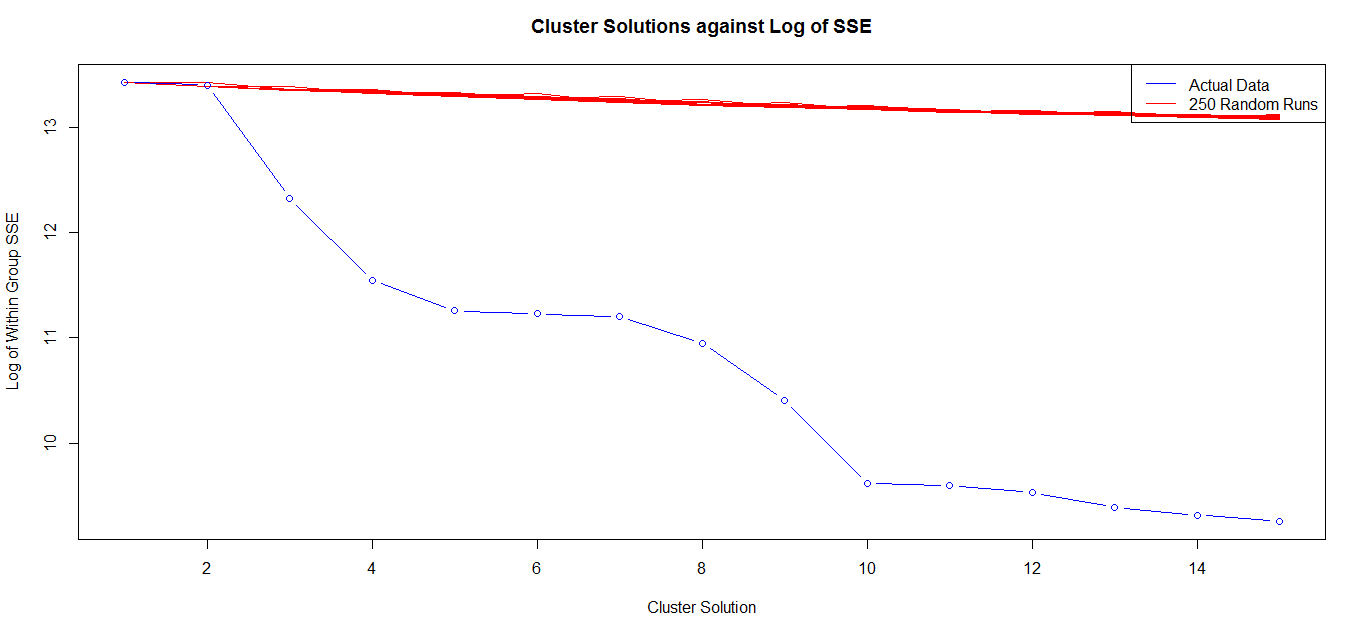
\includegraphics[width=1.0\columnwidth]{figures/SSE1.png}
 \caption{Squared error inside clusters (SEE) as a function of number of clusters for the k-means algorithm}
 \label{dynamicSSE}
\end{figure}

The SSE analysis usually does not yield the direct answer.
The tool provides several plots, but the most interesting one is presented in Fig.~\ref{dynamicSSE}. 
Looking at this plot, there is a significant drop in SSE for the cluster numbers equal to $5$ and $10$.
It is expected that either of those numbers is the correct choice when it comes to the number of classes for k-means algorithm.

\begin{table}[htbp!]
 \caption{Comparison of suggested number of clusters for the dataset containing all positions of hand in all dynamic gesture recordings made by Katarzyna}
 \label{clusterwyn}
    \begin{tabular}{ccccc}
    \hline
     & Girven-Newman & Chinese whispers   & SSE vs clusters & Silhouette width  \\ \hline
    recordings \\by Katarzyna          & no convergence      & $613$ & $5$ or $10$     & $4$     \\ \hline
    \end{tabular}
\end{table}

The Silhouette width approach run on the same data estimated that the there are $4$ distinguishable clusters.
The Girvan-Newman algorithm did not provide any estimate within $24$ hours and therefore was considered impractical.
Chinese whispers algorithm with typical parameters estimated that data contained $613$ clusters.
The proposed values of clusters for different methods are presented in the Table~\ref{clusterwyn}.

Due to the inconclusive results, the analysis of the correct class number was postponed until the correct feature set is chosen.
Until stated otherwise, the class number was assumed to be equal to $10$.

\subsection{Testing different feature sets}
The next challenge was to find the feature set describing one gesture in time, that would contain all necessary information about the dynamic nature of the gesture. 
All performed tests were evaluated on the dynamic 6 set described in Section~\ref{dynamic:set}.

The first feature set consists of features encoding the information about the speed of the hand. 
For each $i$-th hand position in recorded sequence, the $(i-10)$-th position was also considered. 
The feature set consisted of the recorded displacement of hand in $X$, $Y$, $Z$ directions.
The number of fingers is also added to feature set containing:
\begin{itemize}
\item a finger count in $i$-th hand position,
\item a finger count in $i-10$-th hand position,
\item a displacement of a hand position in $X$ axis,
\item a displacement of a hand position in $Y$ axis,
\item a displacement of a hand position in $Z$ axis.
\end{itemize}
The presented approach allowed to achieve $64.6\%$ on cross-validation set of the dynamic 6 set. 
Due to the small number of samples in the testing set, the total recognition rate was calculated on all available data from the dynamic 6 set.
Using all samples recognition rate was equal to $61.8\%$, which is too small to by used in real applications.

The analysis revealed that previous approach suffered from the fact, that the encoded speeds are represented in the coordinate system of the Leap Motion.
Executing the gesture with different angle to the Leap Motion's coordinate system makes the feature set completely different and sometimes results in mislabelling.
Therefore, the feature set was supposed to encode the information with respect to the local coordinate system of hand. 
In new approach, a magnitude of the displacement is calculated. 
It is independent of the chosen orientation of the coordinate system.
To represent the direction of movement, the normalized displacement vector is computed as a vector connecting the center of $i-10$-th hand position with $i$-th hand position.
Then, the dot product between normalized displacement vector and palm normal in $i-10$ position is calculated.
A dot product between the normalized displacement vector and the palm direction is also computed.
The resulting feature contains:
\begin{itemize}
\item a finger count in $i$-th hand position,
\item a finger count in $i-10$-th hand position,
\item a magnitude of the hand's displacement,
\item a dot product of the normalized displacement vector and the palm's normal in $i-10$-th position,
\item a dot product of the normalized displacement vector and the palm's direction in $i-10$-th position.
\end{itemize}
This approach allowed to improve the recognition rate to $69.6\%$ in a cross-validation and to $67.5\%$ on the whole dynamic 6 set, but was still not satisfying from the practical point of view.

From the observation of changes in the feature set values on the recorded gestures, it was concluded that sometimes only the fingers are changing positions, while position of hand is steady.
The previous approaches, did not encode this information in feature vectors, which made those changes invisible to the further processing part.
Therefore, the new feature vector contains also the information about the displacement of each corresponding finger.
In order to keep the feature size small, it was decided to only incorporate the magnitude of those displacements. 
Due to the nature of Leap Motion's erratic numbering of fingers, those magnitudes were also sorted.
The total of four top values were added to feature vector resulting in feature set:
\begin{itemize}
\item a finger count in $i$-th hand position,
\item a finger count in $i-10$-th hand position,
\item a magnitude of the hand's displacement,
\item a dot product of the normalized displacement vector and the palm's normal in $i-10$-th position,
\item a dot product of the normalized displacement vector and the palm's direction in $i-10$-th position,
\item the $4$ greatest magnitudes of finger displacements.
\end{itemize}
The obtained results were even worse than the ones achieved for the feature set two --- $66.1\%$ compared to the previously achieved $67.5\%$ on the whole dynamic 6 set. 
The further inspection revealed that, while adding displacement of fingers helps in most situations, it can also pose a great risk.
Leap Motion sensor can sometimes change the finger numbering resulting in the displacements calculated between different fingers.
This leads to a big, artificial, phantom displacement.
Therefore, the idea of using a displacement of fingers was abandoned.
 
Looking at the recorded gestures, it seemed that speed information is not sufficient to correctly detect the sequences of gestures combining in one dynamic gesture.
The new feature set contains also the information about the static hand positions allowing to distinguish between dynamic gestures that are comprised of sequential static gestures.
The new feature set contained the already proposed speed part with additional static encoding that was successfully used in static gesture recognition:
\begin{itemize}
\item a finger count in $i$-th hand position,
\item a finger count in $i-10$-th hand position,
\item a magnitude of the hand's displacement,
\item a dot product of the normalized displacement vector and the palm's normal in $i-10$-th position,
\item a dot product of the normalized displacement vector and the palm's direction in $i-10$-th position,
\item the $4$ greatest euclidean distances between all combination of finger's tips in $i$-th position,
\item the $4$ greatest absolute angles between all combination of finger's vectors in $i$-th position,
\item the $4$ greatest euclidean distances between finger's tips and palm's position in $i$-th position,
\item the $4$ greatest absolute angles between finger's vectors and palm's normal in $i$-th position.
\end{itemize}

The experiments showed that the proposed approach allowed to improve recognition rate.
On the other hand, it was believed that the sophisticated static part of feature set is dominating the dynamic part of the feature set, which prevents the method from achieving better results.
Therefore, the $5$-th proposed feature set consists of static part represented only by the $4$ greatest euclidean distances between all combination of finger's tips in $i$-th position and the $4$ greatest absolute angles between all combination of finger's vectors in $i$-th position.
Similarly, feature sets $6$, $7$, $8$ were also the propositions containing the reduced encoding of the static parts, but did not improve significantly over already received results. 
The results obtained by all proposed feature sets are presented in Table~\ref{tab:dyn1}. 

\begin{table}[htbp!]
\begin{center}
	\label{tab:dyn1}
	\caption{Results obtained by the HMM approach using different feature sets}
    \begin{tabular}{ccc}
    \hline
    ~                                 & $5$ gestures, CV & $5$ gestures, whole dataset  \\ \hline
    feature set $1$                     & $64.6\%$ & $61.8\%$   \\ \hline
    feature set $2$                     & $69.6\%$ & $67.5\%$   \\ \hline
    feature set $3$                     & $68.5\%$ & $66.1\%$   \\ \hline
    feature set $4$          		  & $77.9\%$ & $76.1\%$   \\ \hline
    feature set $5$                     & $66.7\%$ & $63.9\%$   \\ \hline
    feature set $6$                    & $72.9\%$ & $70.4\%$   \\ \hline
    feature set $7$                    & $71.9\%$ & $69.2\%$   \\ \hline
    feature set $8$                    & $78.1\%$ & $77.2\%$   \\ \hline
    \end{tabular}
\end{center}
\end{table}
  
The best results were obtained for feature set $8$, but the results obtained by the full static representation (feature set $4$) are not significantly worse.
For further assessment, the feature set $4$ was chosen as the one that describes each gesture with more information and therefore is believed to work better for gestures that were not included in the experiments.

\subsection{Testing number of observation classes} 

The next experiments were performed to test what is the best number of observation classes for k-means algorithm. 
Previous tests to find the correct number of clusters were performed in Subsection~\ref{numberOfClasses1}, but yield inconclusive results.
Therefore, the tests were performed using the processing algorithm to impact of number of classes on the total recognition rate.
The tests were conducted using feature set $4$ and learning rate $\mu=0.05$.

\begin{table}[htbp!]
\begin{center}
	\label{tab:dynNumber}
	\caption{Results obtained by the HMM approach using feature set $4$ and different numbers of class clusters}
    \begin{tabular}{ccc}
    \hline
    ~                                 & $5$ gestures, CV & $5$ gestures, whole dataset  \\ \hline
	$k = 4$                  	  & $77.3\%$ & $74.7\%$   \\ \hline
    $k = 5$               	  & $79.6\%$ & $77.6\%$   \\ \hline
    $k = 6$                    & $79.6\%$ & $77.6\%$   \\ \hline
    $k = 8$                     & $77.7\%$ & $76.0\%$   \\ \hline
    $k = 10$                    & $77.9\%$ & $76.1\%$   \\ \hline
    $k = 12$                    & $78.5\%$ & $77.4\%$   \\ \hline
    \end{tabular}
\end{center}
\end{table}
The results are presented in Table~\ref{tab:dynNumber}.
The best obtained results are for the number of clusters $k=5$ and $k=6$ for which an increase in the recognition rate when compared to the previously achieved results. 
The recognition rate in cross-validation was equal to $79.583\%$ and $77.639\%$ on the dynamic 6 set. 

\subsection{Testing learning rate}

The next experiments involved finding the best learning rate. 
Using predefined learning rate may be dangerous as small value may mean small convergence, while too big step may result in not converging to the locally best solution. 
In our application, the stable learning rate through whole training process was chosen to minimize the number of parameters. 
The further developments may involve using learning rate that is changing depending on the already training error.
The experiments were conducted on the same dataset using feature set four, five observation classes and learning rates:
\begin{itemize}
\item $\mu$ = 0.01
\item $\mu$ = 0.05
\item $\mu$ = 0.1
\item $\mu$ = 0.2
\end{itemize}
The achieved results are presented in Table~\ref{tab:dyn2}.
In proposed application, the learning rate $\mu = 0.05$ allowed to achieve the best results and is recommended by the authors of this thesis. 

\begin{table}[htbp!]
\begin{center}
	\label{tab:dyn2}
	\caption{Results obtained by the HMM approach using feature set $4$, $5$ observation classes and different learning rates}
    \begin{tabular}{ccc}
    \hline
    ~                                 & $5$ gestures, CV & $5$ gestures, whole dataset  \\ \hline
	$\mu$ = 0.01                  	  & $77.5\%$ & $76.9\%$   \\ \hline
    $\mu$ = 0.05                      & $80.4\%$ & $79.0\%$   \\ \hline
    $\mu$ = 0.1                      & $79.6\%$ & $77.6\%$   \\ \hline
    $\mu$ = 0.2                      & $69.6\%$ & $69.7\%$   \\ \hline
    \end{tabular}
\end{center}
\end{table}

\subsection{Testing number of states in HMM}

The only parameter not tested in the already described experiments is the number of state each HMM is composed of. 
The previously used value was equal to $10$ states. 
In the experiments four different values were tested: 5, 10, 20 and 30.
The results from experiments are presented in Table~\ref{tab:dyn3}. 
The performed experiments confirmed that smaller number of states ($5$) results in lower recognition rate as the HMM is not complicated enough to fully learn the presented model of the dynamic gesture.
The number of states greater than 10 did not improve the results achieved using 5 states.
When choosing the number of states, it is also important to remember about the complexity of algorithms, which are grow quadratically with the number of states, which affects the learning and recognition times. 
The performed experiments and theoretical computational complexity confirm that the computational complexity grows quadratically with the chosen number of states.


\begin{table}[htbp!]
\begin{center}
	\label{tab:dyn3}
	\caption{Results obtained by the HMM approach using feature set $4$, $6$ observation classes and a different number of states}
    \begin{tabular}{ccc}
    \hline
    ~                                 & $5$ gestures, CV & $5$ gestures, whole dataset  \\ \hline
	$K = 5$                  	  & $74.0\%$ & $73.6\%$   \\ \hline
    $K = 10$                     & $79.6\%$ & $77.6\%$   \\ \hline
    $K = 20$                    & $77.5\%$ & $76.5\%$   \\ \hline
    $K = 30$                     & $77.9\%$ & $76.2\%$   \\ \hline
    \end{tabular}
\end{center}
\end{table}
\chapter{LMGesture library dedicated for Leap Motion controller}

\section{Architecture}

\subsection{Model}

While data from the LMR files are being processed, they are stored using a specially created class representing the data. GestureFrame represents a single frame obtained from Leap Motion Controller. All gathered data is stored in a vector containing elements of GestureFrame type. GestureFrame holds information such as:

\begin{itemize}
\item timestamp,
\item list of hands occurring in the frame, stored in a vector containing elements GestureHand type.
\end{itemize}

GestureHand stores parameters of hand performing gesture. In one instance of GestureFrame can be stored many instances of GestureHand. GestureHand holds following information:
\begin{itemize}
\item hand id,
\item plam position,
\item stabilized palm position,
\item palm normal vector,
\item palm direction,
\item list of fingers of particular hand, stored in a vector containing elements GestureFinger type,
\item ordered value, obtained during hand sorting.
\end{itemize}

GestureFinger stores parameters of one finger. In one instance of GestureHand can be stored many instances of GestureFinger. GestureFinger contains:
\begin{itemize}
\item finger id,
\item tip position,
\item stabilized tip position,
\item finger direction,
\item finger length,
\item finger width,
\item ordered value, obtained during finger sorting.
\end{itemize}

\section{Processes}

\subsection{The learning process}
The learning process is a process, which shows how user can teach LMGesture library a new gesture. First  gestures must be recorded gestures in LMR format. To obtain recordings in this format user may use Gesture Recorder --  a module included in the library, which records data from Leap Mption Controller and saves it as LMR file. When all desired gestures are prepared, the user starts the process of learning by {\color{red}[tutaj dodać informacje jak uruchomić ten prces - prawdopodobnie jakas komenda + jakies parametry typu -d uczenie gestów dynamicznych, -s uczenie gestów statycznych + pliki LMR jako argumenty]}. 

\begin{figure}[htb]
\centering
 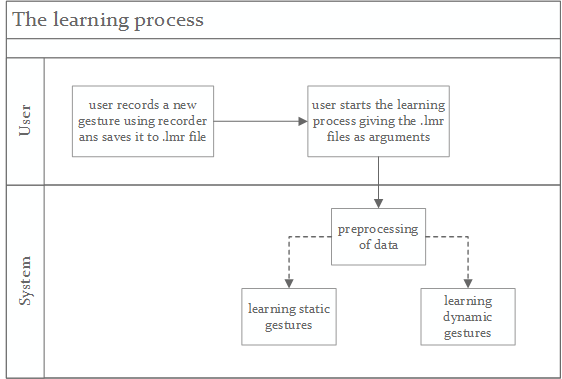
\includegraphics[width=0.75\columnwidth]{figures/learningProcess.png}
 \caption{Diagram showing the learning process}
 \label{learningprocess}
\end{figure}

The first step in the learning process, which is performed by the system is the preprocessing of data. Training data should be deprived of noise or should not have lost fingers for several frames. According to user-specified parameters, the system will learn the gesture as a static or dynamic gesture. Appropriate way of learning corresponds to the appropriate gesture.
For the learning static gesture system uses a support vector machine (SVM), and for dynamic gestures uses hidden Markov model (HMM). 
The learning process for static gestures:
\begin{enumerate}
\item In the first stage, data which will be used during the learning is preprocessed.
\item Data are scaled using internal scaling module. The result of this step are scale and range files. In the scale file scaled data is stored. The range file contains information that enables to scale any data in the same way.
\item Scale file with scaled data is transmitted to training module. Data is processed using SVM algorithm. Additionally during learning process k-validation is performed and results are returned to the user. In process model file is created, which is used during static gesture recognition process.
\end{enumerate}
{\color{red}[opisać learning process dla dynamicznych]}


\subsection{The recognition process}
The recognition process is a process in which the system attempts to match gesture given by a user, to the set of gestures obtained by the learning process. {\color{red}[Opis procesu recognition process, przedstawienie scenariusza uzycia w stosunku do architektury]}

\begin{figure}[htb]
\centering
 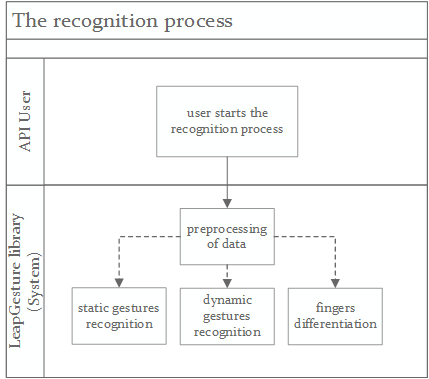
\includegraphics[width=0.6\columnwidth]{figures/recognitionProcess.png}
 \caption{Diagram showing the recognition process}
 \label{recognitionprocess}
\end{figure}

Modules handlers are implemented using the Observer pattern. For each of the modules are specified relevant events that are reported in the key moments of recognition such as: moment in which particular gesture began to be recognized, moment in which the particular gesture stopped being recognized, moment in which frame processing is finished.
The user can handle events received in specific module by implementing appropriate listener interface and adding reference to listener list in specific library module. During gesture recognition process user can use from 1 to 3 listeners. Each listener is on a separate thread.

Methods for a static gesture observer:
\begin {itemize}
\item onStart -- signals the start of the gesture,
\item onFrame -- returns a list of recognized gestures with matching probabilities,
\item onGesture -- signals the end of the gesture and returns a list of recognized gestures with matching probabilities.
\end {itemize}

Methods for a dynamic gesture observer:
\begin {itemize}
\item onStart, onFrame -- have the same purposes as in the case of static observer,
\item onGesture -- signals the end of the gesture and returns a list of recognized gestures with matching probabilities and parameter values.
\end {itemize}

Methods for a finger differentiation observer:
\begin {itemize}
\item onFrame -- returns a list of matched classes with probabilities,
\item onChange -- signals a change of fingers arrangement.
\end {itemize}

As in the learning process for recognizing static gestures system uses SVM and for dynamic gestures -- HMM. For finger differentation system uses support vector machine. However, there are other classes than those used for static gestures recogniton.

\section{Gesture recorder and visualizer}
Recorder and vizualizer module is an additional part of library that allows users for easy management of gestures recordings. The recorder collects data from Leap Motion Controller, converts it into data representation described in section regards architecture of library {\color{red}[weryfikacja po skleceniu pracy]} and writes it to the LMR file, which is supported by the LMGesture library. Visualizer enables users to see the recorded gestures stored in LMR format. Data gathered from Leap Motion, used to recognize gestures are very large and the data processed in the library have a specific format. Therefore, it was necessary to create an auxiliary program, that it would facilitate the work with data in the fastest and most user-friendly way.

\subsection{LMR files}
This is a file format specially developed for the LMGestue library, supported by various modules for example by the visualizer. The file structure is as follows:
\begin{itemize}
\item Line represents one frame.
\item One frame contains: timestamp and hand parameters.
\item Hand parameters include: hand id, palm position, stabilized palm position, palm normal vector, palm direction vector and detected fingers parameters.
\item Finger parameters include: finger id, finger tip position, stabilized tip position, finger direction vector, finger length and finger width.
\end{itemize}

Technical information regards LMR files:
\begin{itemize}
\item Timestamp and hands are separated by ``\#''. 
\item In specified hand occurs hand parameters and fingers. 
\item Hand parameters are separated by space, and finger are separated by ``f'' (hands parameters and fingers are separated by ``f'' too). 
\item Specified finger has parameters, which are splited by `` ''. 
\item Values in the trivalent parameters are separated by a semicolon.
\end{itemize}

\subsection{Visualizer}
Visualizer presents the contents of the lmr files. As mentioned earlier, each line of the file is a separately converted frame obtained from Leap Motion Controller. In one moment only one frame is displayed.
Almost all fields of the model are visualized:
\begin{itemize}
\item palm position,
\item palm normal vector,
\item palm direction,
\item tip position,
\item finger direction,
\item finger length.
\end{itemize}

\begin{figure}[htb]
\centering
 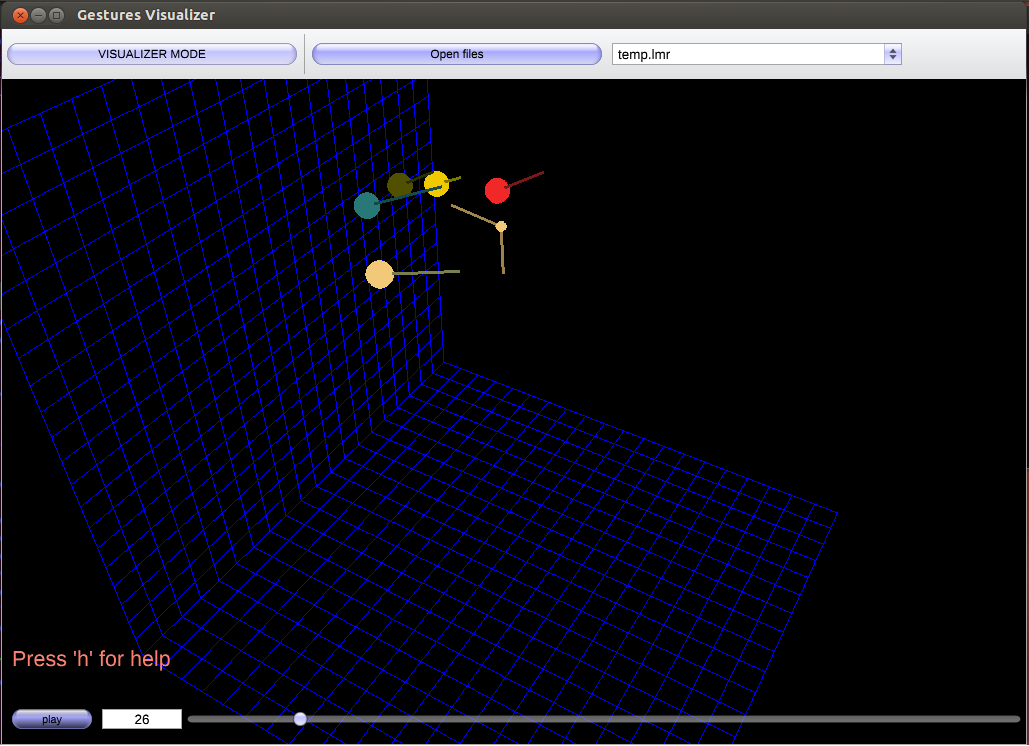
\includegraphics[width=1\columnwidth]{figures/visualizer.png}
 \caption{Screenshot of the visualizer}
 \label{visualizer}
\end{figure}

An example of parameter, which is not visualized, is finger width, in order not to obscure the image.
\begin{itemize}
\item Program can read the lmr files chosen by the user.
\item The user can load many files at once and select one of the recordings from the drop-down list.
\item To facilitate the user work with visualizer, program has implemented windowing interface.
\item The user has ability to rotate and zoom camera.
\item Slider is available in order to move between frames of the recording.
\item Visualizer has option to play recorded gesture, which the user can turn on and off by pressing the play/stop button.
\item There is also a button to enter the recorder mode.
\end{itemize}

\subsection{Recorder}
Recorder is part of the described module, which is responsible for collecting information from Leap Motion Controller and saving it to lmr file.
Each frame read from the Leap Motion is captured, and then converted to the previously described model. Then the model is saved by the appropriate sub-module to LMR file. The conversion process contains also sorting hands and fingers. Hands are sorted by X coordinate of palmPosition. In the case of sorting fingers, the usual sort by X coordinate is not enough. The order of the fingers must be independent of hand rotation, therefore a different method for fingers sorting had to be proposed. Fingers are sorted by distance between finger tip position and plane, which is perpendicular to the surface of the hand and contains a direction vector of a hand. This plane can be determined using palm position, direction vector and normalized normal vector of the hand.
Below is the formula for the distance ($d$) between finger tip position and designated plane.

\[ d = -(f - pp) \cdot (\hat{hd} \times \hat{hn}) \]
Where:
\begin{itemize}
    \item[] $f$: is the finger tip position
    \item[] $pp$: is the palm position
    \item[] $hd$: is the hand direction vector
    \item[] $hn$: is the hand normal vector
\end{itemize}

List of Recorder features:
\begin{itemize}
\item Turning on and off recording is done by using space key.
\item After recording window automatically appears, in which can be choosen where to save the file.
\item The recorder cooperates with the visualizer. During recording performed gesture is visualized.
\item There is a button to enter the visualizer mode.
\end{itemize}

\begin{figure}[htb]
\centering
 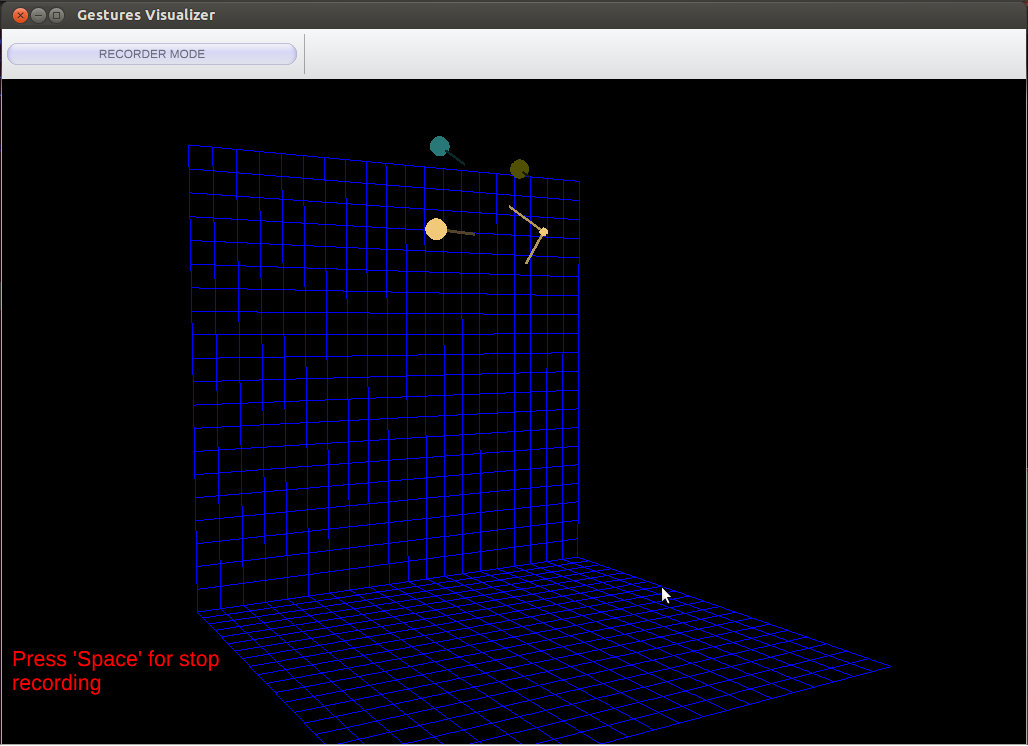
\includegraphics[width=1\columnwidth]{figures/recorder.png}
 \caption{Screenshot of the recorder}
 \label{recorder}
\end{figure}

\section{Used libraries}

\section{Samples of code using the library dedicated to Leap Motion Controller}

\chapter{Conclusions}\label{conclusionsChapter}

This thesis describes LeapGesture, which is the hand gesture recognition library dedicated for Leap Motion Controller.
This library includes modules for static and dynamic gesture recognition and also finger recognition.
Developed library provides recognition of all types of action gestures.
Static action gestures are supported by static gesture processing thread, while the dynamic gesture processing thread provides recognition of dynamic action gestures.
Additionally, comparison of existing gesture recognition methods, implementation of additional modules enabling the recording and reviewing of gestures, creation of sample gestures database and performation of tests has been conducted.
%This thesis contains a thorough evaluation of proposed approaches to the gesture recognition.

The results obtained for the static gesture recognition suggest than those gestures are easy to recognize using the SVM with appropriate pre and postprocessing.
The differences between the recognition rates for different feature sets even values reaching up to $13\%$ show that choosing different feature sets can have a major impact on the performance of recognition.
Additionally, it is important not to undermine the influence of the data preprocessing. 
Even the usage of the relatively simple median filter allowed to boost the recognition rate by $6\%$.
Although, the authors believe that the proposed parameters of processing module work well in many scenarios, there might be some specific cases that need different parameters or different feature sets to achieve good results.
It is also worth noting, that this and any another approach will not work properly if during the performance of static gestures, hands and fingers are not correctly detected by the Leap Motion.
Therefore it is recommended to always choose gestures that have visible and separated fingers from the sensor's perspective.
For the proposed approach, recognition rate of $99\%$ for five classes of gestures and $85\%$ for ten classes of gestures in the static gesture recognition task were achieved. Satisfactory results of $93\%$ were also obtained for the task of finger recognition for $15$ of $32$ classes of fingers arrangements.

When it comes to the task of dynamic gestures recognition, Leap Motion might not be the best sensor choice.
Leap Motion provides great accuracy for static hand and fingers, but the data for dynamically moved hands are usually noisy.
The problems arise with short, lost finger tracking or temporal finger occlusions that are hard to detect and cope with on the library-level.
The proposed preprocessing module tries to alleviate those negative impacts, but the preprocessed data is still far from ideal.
Nevertheless the proposed approach with Hidden Markov Models allowed to recognize five classes of dynamic gestures with $80\%$ accuracy.

As part of the further development of the library, the authors intend to improve the efficiency of dynamic gesture recognition by testing other possible feature sets and to develop methods that will allow to preprocessed data derived from Leap Motion more efficiently. Supporting of parameterized gestures is also envisaged.



% All appendices and extra material, if you have any.
\cleardoublepage\appendix%
%\input{0a-appendix.tex}

% Bibliography (books, articles) starts here.
\bibliographystyle{plain}{\raggedright\sloppy\small\bibliography{bibliography}}

% Colophon is a place where you should let others know about copyrights etc.
\ppcolophon

\end{document}
